\documentclass[10pt,a4paper,twocolumn]{article}

% --- Geometria della Pagina e Layout ---
\usepackage[top=2.0cm,bottom=2.0cm,left=1.8cm,right=1.8cm,columnsep=0.65cm]{geometry}

% --- Codifica, Font e Microtipografia ---
\usepackage[utf8]{inputenc}
\usepackage[T1]{fontenc}
\usepackage{mathptmx}
\usepackage{microtype}

% --- Pacchetti Matematici Avanzati ---
\usepackage{amsmath,amssymb,amsfonts,amsthm}
\usepackage{mathtools}
\usepackage{bm}

% --- Tabelle e Figure ---
\usepackage{booktabs}
\usepackage{tabularx}
\usepackage{multirow}
\usepackage{graphicx}
\usepackage{subcaption}
\usepackage{float}

% --- Algoritmi ---
\usepackage{algorithm}
\usepackage{algorithmic}

% --- Collegamenti Ipertestuali e Riferimenti ---
\usepackage[numbers,sort&compress]{natbib}
\usepackage[colorlinks=true,
            linkcolor=blue!70!black,
            citecolor=blue!70!black,
            urlcolor=blue!70!black,
            pdfencoding=auto,
            psdextra]{hyperref}

% --- Ambienti Matematici Teorema / Definizione ---
\newtheorem{theorem}{Theorem}[section]
\newtheorem{lemma}[theorem]{Lemma}
\newtheorem{definition}[theorem]{Definition}
\newtheorem{remark}[theorem]{Remark}

% --- Titolo e Autori ---
\title{\textbf{\Large Graph Dynamic Meshing (GDM): A Conservative and Safety-Guaranteed Neural Adaptive Mesh Framework for Transient Convection-Diffusion PDEs}}

\author{
  \textbf{Giovanni Giuseppe Iacuzzo}\textsuperscript{1,*} \\
  \small \textsuperscript{1}Department of Engineering and Architecture, University of Enna "Kore", Enna, Italy \\
  \small \textsuperscript{*}Corresponding author: \texttt{giovanni.iacuzzo@unikore.it}
}

\date{\today}

% -------------------------------------------------------------
% INIZIO DOCUMENTO
% -------------------------------------------------------------
\begin{document}

\maketitle

% --- Abstract ---
\begin{abstract}
\noindent
% Sintesi sintetica: contesto del problema (mesh r-adaptation e FEM transiente),
% limiti dei metodi correnti (costo dell'ottimizzazione variazionale runtime,
% degradazione da remapping pointwise, instabilità geometrica / inversioni di celle),
% framework proposto (GDM: GNN + filtro analitico di non-inversione + formulazione ALE D-GCL conforme),
% principali risultati quantitativi (speedup rispetto a ottimizzatori classici, conservazione massa/GCL, accuratezza PDE).
\textit{Abstract placeholder: contesto, problema aperto, metodologia proposta (GDM), proprietà teoriche (D-GCL, invariabilità topologica, safety filter), risultati chiave e speedup computazionale.}
\end{abstract}

\vspace{0.5em}
\noindent\textbf{Keywords:} Adaptive Mesh Refinement, $r$-adaptation, Graph Neural Networks, Arbitrary Lagrangian-Eulerian (ALE), Geometric Conservation Law, Finite Element Method.
\newpage

% =============================================================
% 1. INTRODUZIONE
% =============================================================
\section{Introduction}
\label{sec:introduction}
\subsection{Contesto e motivazione}

La simulazione numerica accurata ed efficiente di equazioni alle derivate parziali (Partial Differential Equations, PDE) dipendenti dal tempo costituisce un elemento centrale della matematica computazionale e dell'ingegneria scientifica \citep{quarteroni2009the}. In numerosi problemi applicativi, quali il trasporto convettivo, la fluidodinamica e la diffusione di quantità fisiche in presenza di strutture spaziali localizzate, la soluzione può presentare gradienti ripidi, fronti mobili e regioni caratterizzate da scale spaziali molto differenti \citep{donea2003finite}. In tali condizioni, una discretizzazione uniforme e statica può risultare fortemente inefficiente, poiché per risolvere adeguatamente le strutture più piccole è necessario mantenere un'elevata risoluzione anche nelle regioni del dominio in cui la soluzione varia lentamente.

L'adattività della discretizzazione costituisce una delle principali strategie per affrontare questo problema \citep{bangerth2003adaptive}. L'obiettivo è distribuire i gradi di libertà in modo non uniforme, aumentando la risoluzione nelle regioni in cui la soluzione presenta maggiore complessità e riducendola altrove. Nell'ambito dei metodi agli elementi finiti (Finite Element Method, FEM), tale principio può essere perseguito attraverso differenti forme di adattività, tra cui $h$-, $p$- e $r$-refinement.

\subsection{\texorpdfstring{Adattività di griglia e ($r$-refinement)}{Adattività di griglia e(r-refinement)}}

Nel caso dell'$h$-refinement, la risoluzione viene modificata attraverso la suddivisione o il riaccorpamento locale degli elementi, determinando una variazione del passo di discretizzazione e, generalmente, del numero di gradi di libertà \citep{berger1984adaptive}. Sebbene tale approccio sia ampiamente consolidato, nelle simulazioni transitorie caratterizzate da frequenti eventi di adattamento la variazione della connettività può introdurre costi aggiuntivi associati alla gestione della mesh, alla costruzione dei sistemi sparsi e, in implementazioni parallele, al bilanciamento del carico.

Il $p$-refinement modifica invece localmente l'ordine polinomiale delle funzioni di forma mantenendo invariata la geometria degli elementi \citep{szabo2021finite}. Esso può risultare particolarmente efficace per soluzioni sufficientemente regolari, mentre la sua efficacia può ridursi in presenza di strutture non lisce o di forti localizzazioni della soluzione.

L'$r$-refinement, o \textit{moving mesh adaptation}, adotta una strategia differente: il numero di nodi e la connettività topologica vengono mantenuti fissi, mentre le coordinate dei nodi vengono adattate nel tempo per concentrare la risoluzione nelle regioni di maggiore interesse \citep{huang2010adaptive,budd2009adaptivity,hyman1988moving}. Questa caratteristica rende l'$r$-refinement particolarmente interessante per problemi transitori, poiché consente di modificare la distribuzione spaziale dei gradi di libertà senza alterare la dimensione del sistema algebrico associato alla discretizzazione.

I metodi classici di moving mesh determinano generalmente la nuova configurazione della mesh attraverso formulazioni variazionali, principi di equidistribuzione o equazioni ausiliarie per il moto della griglia, tra cui le Moving Mesh Partial Differential Equations (MMPDE) \citep{huang2001practical,huang2010adaptive,budd2009adaptivity}. Sebbene tali formulazioni siano consolidate e possano produrre mesh di elevata qualità, il calcolo della configurazione adattata costituisce un problema aggiuntivo rispetto alla PDE fisica. Quando l'adattamento deve essere eseguito frequentemente, il costo della procedura di mesh movement può quindi diventare una componente significativa del tempo complessivo di simulazione \citep{song2022m2n,rowbottom2024g}.

\subsection{Metodi di mesh movement basati su apprendimento automatico}

Lo sviluppo dello Scientific Machine Learning e del Geometric Deep Learning ha recentemente motivato l'impiego di modelli neurali per apprendere operatori definiti direttamente su mesh non strutturate e grafi \citep{bronstein2021geometric,battaglia2018relational}. In questo contesto, una mesh agli elementi finiti può essere rappresentata naturalmente mediante un grafo i cui nodi corrispondono ai gradi di libertà geometrici e i cui archi codificano le relazioni di adiacenza.

Un primo filone di lavori ha mostrato che reti neurali possono essere utilizzate per sostituire, o accelerare, le procedure classiche di mesh movement. M2N, ad esempio, introduce un framework basato su apprendimento automatico per la rilocazione dei nodi e considera esplicitamente problematiche quali il mesh tangling, la consistenza al bordo e la generalizzazione a differenti risoluzioni; il metodo viene validato sia su problemi stazionari sia su problemi tempo-dipendenti \citep{song2022m2n}. Successivamente, DMM e il relativo framework MM-PDE hanno proposto un mesh mover basato su una formulazione neurale della mappa di adattamento, mantenendo fissi i nodi esistenti e integrando il movimento della mesh all'interno di un solutore per PDE dinamiche \citep{hu2024better}.

Un ulteriore sviluppo è rappresentato da UM2N, che impiega un'architettura basata su Graph Transformer e Graph Attention Network per apprendere il movimento della mesh e ne studia l'applicabilità a differenti PDE, geometrie e risoluzioni, includendo problemi di advezione e Navier--Stokes \citep{zhang2024towards}. Più recentemente, G-Adaptivity ha formulato direttamente il problema della rilocazione dei nodi nel contesto FEM come un problema di apprendimento mediante GNN, ottimizzando la posizione dei nodi in funzione dell'errore della soluzione agli elementi finiti e mirando a ridurre il costo delle procedure classiche di adattamento \citep{rowbottom2024g}. Un lavoro recente ha inoltre studiato l'impiego di reti neurali per $r$-adaptive FEM in problemi ellittici autoaggiunti parametrizzati, evidenziando tuttavia un'impostazione specifica per problemi coercivi e per mesh aventi struttura tensoriale \citep{aballay2026radaptive}.

Nel loro insieme, questi lavori mostrano che il machine learning può ridurre significativamente il costo della generazione di mesh adattive e che le GNN costituiscono una scelta naturale per operare direttamente sulla struttura della discretizzazione. Essi mostrano inoltre che la gestione della qualità geometrica della mesh rappresenta una componente essenziale dei metodi neurali di mesh movement. In particolare, il problema della possibile inversione o degenerazione degli elementi è stato affrontato mediante differenti strategie, tra cui trasformazioni neurali strutturalmente invertibili, termini di perdita geometrici e architetture progettate per limitare il mesh tangling \citep{song2022m2n,zhang2024towards}.

Questi risultati evidenziano tuttavia una distinzione importante. La predizione di una nuova configurazione della mesh non specifica, di per sé, come l'evoluzione della soluzione numerica debba essere trattata quando la geometria cambia nel tempo. In particolare, occorre distinguere tra una sequenza di rilocazioni discrete della mesh, che richiede il trasferimento dello stato numerico tra spazi FEM differenti, e una formulazione in cui il movimento della mesh entra direttamente nell'integrazione temporale della PDE.

\subsection{Remapping, mesh mobile e formulazione ALE}

Quando una procedura di adattamento produce una nuova configurazione $\mathcal{T}^{n+1}$ a partire da $\mathcal{T}^{n}$ mediante una rilocazione discreta dei nodi, lo stato numerico rappresentato sulla mesh precedente deve essere trasferito al nuovo spazio discreto. Indicando con $u^n_{\mathcal{T}^n}$ la soluzione numerica sulla configurazione precedente, il trasferimento assume schematicamente la forma
\[
u^n_{\mathcal{T}^n}
\longrightarrow
u^n_{\mathcal{T}^{n+1}}.
\]
Tale operazione di \textit{state remapping} introduce un ulteriore operatore numerico nella pipeline e, nel caso di simulazioni con numerosi eventi di adattamento, il relativo errore può accumularsi nel tempo. La scelta dell'operatore di trasferimento è pertanto parte integrante della qualità numerica complessiva del metodo.

Una possibile strategia consiste nell'utilizzare un'interpolazione nodale o elementare; un'alternativa più accurata è rappresentata dalla proiezione variazionale, ad esempio mediante una proiezione in norma $L^2$, che consente di trasferire lo stato imponendo una condizione di ortogonalità rispetto al nuovo spazio FEM. Tuttavia, una proiezione di questo tipo richiede la costruzione e la soluzione di un sistema associato alla nuova matrice di massa, introducendo un costo algebrico non trascurabile. La questione non consiste quindi soltanto nell'ottenere una mesh adattata, ma nel determinare come evolvere la soluzione numerica durante il movimento della discretizzazione senza introdurre un costo di trasferimento eccessivo.

Una formulazione alternativa è costituita dal paradigma Arbitrary Lagrangian--Eulerian (ALE), nel quale la mesh viene descritta mediante una mappa tempo-dipendente
\[
\mathbf{x}=\mathbf{x}(\boldsymbol{\xi},t)
\]
e il suo moto è caratterizzato dalla velocità di griglia
\[
\mathbf{w}=\frac{\partial \mathbf{x}}{\partial t}.
\]
La velocità della mesh modifica direttamente i termini convettivi della formulazione differenziale, evitando di trattare il cambiamento della configurazione come una successione di trasferimenti indipendenti dello stato \citep{hirt1974an,donea2004arbitrary}.

L'impiego di una mesh mobile introduce tuttavia una condizione di consistenza geometrica fondamentale. La discreta evoluzione della geometria e l'integrazione temporale della PDE devono essere compatibili con la Geometric Conservation Law (GCL), affinché un campo uniforme possa essere preservato durante il moto della griglia. Nel contesto FEM-ALE, la D-GCL (Discrete Geometric Conservation Law) fornisce quindi una condizione discreta per la corretta rappresentazione dell'evoluzione geometrica e per la preservazione di stati uniformi sulla mesh deformante \citep{farhat2001the,formaggia2004stability}.

È importante distinguere tale proprietà dalla conservazione delle grandezze fisiche della PDE: la verifica della D-GCL e della preservazione del campo costante costituisce una verifica della consistenza geometrica della discretizzazione mobile, e non una dimostrazione generale di conservazione fisica di massa, quantità di moto o energia.

\subsection{Problema aperto e obiettivo del lavoro}

La letteratura esistente ha quindi sviluppato, da un lato, metodi classici e neurali per la generazione e la rilocazione di mesh adattive e, dall'altro, formulazioni FEM-ALE mature per la soluzione di PDE su griglie deformanti \citep{budd2009adaptivity,song2022m2n,hu2024better,zhang2024towards,rowbottom2024g}. Questi filoni affrontano tuttavia problemi differenti: i metodi di mesh movement learning-based si concentrano principalmente sulla predizione della configurazione geometrica adattata e sul costo della procedura di mesh adaptation, mentre la formulazione ALE riguarda il modo in cui il moto della geometria viene incorporato nel solutore differenziale.

Nella letteratura da noi esaminata non abbiamo identificato una pipeline FEM transiente che combini esplicitamente tre componenti in un unico processo numerico: 
(i) la predizione neurale del movimento nodale mediante una GNN;
(ii) una verifica geometrica deterministica e indipendente dalla rete che certifichi l'ammissibilità dello spostamento rispetto alla positività del Jacobiano elementare;
e (iii) l'integrazione del moto predetto come velocità di griglia in una formulazione ALE continua verificata rispetto alla D-GCL, evitando il ricorso al remapping esplicito dello stato ad ogni evento di adattamento.

L'obiettivo del presente lavoro è quindi studiare questa integrazione in modo sistematico, non assumendo a priori che ciascuna componente sia sufficiente isolatamente. Il framework proposto viene pertanto analizzato attraverso una sequenza di verifiche disaccoppiate, finalizzate a distinguere l'errore associato alla predizione della mesh, quello introdotto dal trasferimento dello stato e quello associato alla discretizzazione su mesh mobile.

\subsection{Contributi del lavoro}

In questo articolo presentiamo \textit{Graph Dynamic Meshing} (GDM), un framework ibrido neurale e numerico per l'$r$-adattività di mesh bidimensionali non strutturate a topologia fissa. Il framework combina un modello GNN per la predizione del movimento della mesh, un controllo geometrico deterministico post-inferenza e una formulazione ALE per l'evoluzione della soluzione sulla griglia mobile.

I principali contributi del lavoro sono:

\begin{enumerate}

    \item \textbf{Predizione neurale del movimento nodale:}
    sviluppiamo una rete neurale su grafi che opera direttamente sulla struttura della mesh e predice gli spostamenti nodali sulla base di informazioni geometriche e fisiche disponibili durante la simulazione. La procedura consente di sostituire, in fase di inferenza, la risoluzione iterativa dell'oracolo variazionale con una singola valutazione del modello. Lo scaling computazionale dell'inferenza viene inoltre analizzato sperimentalmente al variare della dimensione della mesh.

    \item \textbf{Filtro geometrico deterministico post-inferenza:}
    introduciamo un \textit{Deterministic Safety Filter} separato dalla rete neurale. Per elementi triangolari lineari e per una traiettoria lineare dello spostamento, il determinante Jacobiano, equivalente alla variazione dell'area orientata, è una funzione quadratica del fattore di scala $\alpha$. Le sue radici possono quindi essere analizzate in forma chiusa per determinare il massimo fattore globale di contrazione ammissibile, garantendo
    \[
    \min_{e} J_e(\alpha) \geq \epsilon>0
    \]
    lungo la traiettoria considerata. La procedura fornisce quindi una verifica geometrica deterministica dell'output neurale, indipendente dalla funzione di perdita utilizzata durante l'addestramento.

    \item \textbf{Accoppiamento con una formulazione ALE continua:}
    trasformiamo lo spostamento nodale predetto in una velocità di griglia e integriamo il relativo moto direttamente nel solutore FEM mediante una formulazione ALE. In questo modo il cambiamento della geometria non richiede, nella pipeline ALE principale, un remapping esplicito dello stato numerico. La consistenza geometrica della formulazione viene verificata mediante test dedicati di D-GCL e di preservazione di un campo uniforme.

    \item \textbf{Validazione numerica disaccoppiata:}
    conduciamo una campagna di esperimenti su una PDE di convezione--diffusione transiente con Manufactured Solution, separando sistematicamente la verifica del mesh mover, del filtro geometrico, degli operatori di remapping e della formulazione ALE. Vengono inoltre analizzati gli ordini di convergenza spaziale e temporale, la sensibilità alla frequenza di adattamento e il costo computazionale delle differenti componenti.

\end{enumerate}

\subsection{Organizzazione del paper}

Il resto dell'articolo è organizzato come segue.

La Sezione~\ref{sec:formulation} presenta la formulazione matematica della PDE di riferimento, la discretizzazione mediante elementi finiti $P_1$ con time-stepping Backward Euler e la definizione del funzionale variazionale utilizzato come oracolo per la generazione dei target di adattamento.

La Sezione~\ref{sec:gdm_framework} descrive il framework GDM, includendo la rappresentazione della mesh come grafo, l'architettura della rete \textit{MeshMoverGNN} e la derivazione del Deterministic Safety Filter.

La Sezione~\ref{sec:ale_dgcl} introduce la formulazione ALE utilizzata per l'evoluzione su mesh mobile e presenta la relativa verifica della D-GCL. La sezione discute inoltre il ruolo del remapping nei metodi a rilocazione discreta e la sua sostituzione, nella pipeline ALE, mediante l'evoluzione continua della geometria.

La Sezione~\ref{sec:diagnostics} riporta le campagne di verifica disaccoppiata dei singoli sottosistemi, comprendendo i risultati relativi al mesh mover, al filtro geometrico, al remapping e alle proprietà di convergenza della discretizzazione.

La Sezione~\ref{sec:dynamic_benchmark} presenta il benchmark dinamico finale e il confronto tra le differenti strategie di adattamento e di evoluzione della mesh, analizzando accuratezza della soluzione, errore integrato nel tempo e costo computazionale.

La Sezione~\ref{sec:discussion} discute i risultati, i compromessi tra accuratezza e costo computazionale e le principali limitazioni dell'attuale formulazione.

Infine, la Sezione~\ref{sec:conclusions} riassume i risultati ottenuti e delinea le prospettive di sviluppo verso problemi più complessi e PDE non lineari.

\newpage

% =============================================================
% 2. MODELLO MATEMATICO E METODI NUMERICI
% =============================================================
\section{Mathematical Formulation and Numerical Discretization}
\label{sec:formulation}

\subsection{Governing PDE: Transient Convection-Diffusion}
\label{subsec:pde_governing}
% Equazione di convezione-diffusione instazionaria 2D su Omega x (0, T].
% Condizioni al contorno di Dirichlet e condizioni iniziali.
% Formulazione MMS (Manufactured Solutions) per verifica esatta analitica.

\subsection{\texorpdfstring{Standard $P_1$ Finite Element Discretization}{Standard P1 Finite Element Discretization}}
\label{subsec:fem_discretization}
% Forma debole spaziale con elementi finiti lineari su triangoli.
% Discretizzazione temporale BDF1 (Backward Euler).
% Proprietà asintotiche attese di convergenza: O(h^2) in L2, O(h) in H1, O(dt) nel tempo.

\subsection{\texorpdfstring{Variational $r$-Adaptation and Oracle Formulation}{Variational r-Adaptation and Oracle Formulation}}
\label{subsec:oracle_formulation}
% Funzionale multiobiettivo continuo: termine di concentrazione gradiente/errore di interpolazione + regolarizzazione di qualità geometrica/distorsione.
% Problema vincolato di ottimizzazione non lineare (L-BFGS-B con barriera) come Oracle di riferimento upper-bound.

\newpage

% =============================================================
% 3. FRAMEWORK GRAPH DYNAMIC MESHING (GDM)
% =============================================================
\section{The Graph Dynamic Meshing Framework}
\label{sec:gdm_framework}
Il framework \textit{Graph Dynamic Meshing} (GDM) è concepito come un livello di adattamento geometrico posto tra il solutore FEM e la discretizzazione spaziale. A partire dalla configurazione corrente della mesh e dalle informazioni fisiche disponibili sulla soluzione numerica, il framework predice uno spostamento nodale che modifica la distribuzione dei gradi di libertà mantenendo invariata la connettività della triangolazione.

La procedura è composta da due stadi distinti. Nel primo, una rete neurale su grafi (\textit{Graph Neural Network}, GNN) apprende la relazione tra lo stato corrente della simulazione e lo spostamento nodale fornito dall'oracolo variazionale descritto nella Sezione~\ref{subsec:oracle_formulation}. Nel secondo, lo spostamento predetto viene sottoposto a un controllo geometrico deterministico indipendente dalla rete, denominato \textit{Deterministic Safety Filter}, che verifica la validità della configurazione risultante e, quando necessario, contrae globalmente lo spostamento prima della sua applicazione alla mesh.

La separazione tra predizione e certificazione geometrica è un elemento strutturale del framework. La GNN è infatti utilizzata come approssimatore veloce dell'operatore di adattamento, mentre la validità geometrica non viene affidata esclusivamente alla funzione di perdita o alle proprietà statistiche del modello appreso. Questa impostazione si colloca nel solco dei recenti metodi learning-based per mesh movement, ma introduce una distinzione esplicita tra la previsione neurale dello spostamento e la successiva verifica deterministica della configurazione geometrica \citep{song2022m2n,zhang2024towards,rowbottom2024g}.

\subsection{Rappresentazione della mesh come grafo}

\label{subsec:graph_representation}

Sia
\[
\mathcal{T}_h=(\mathcal{V},\mathcal{K})
\]
una triangolazione bidimensionale del dominio, dove $\mathcal{V}$ denota l'insieme dei nodi e $\mathcal{K}$ l'insieme degli elementi triangolari. La mesh viene rappresentata mediante un grafo diretto
\begin{equation}
\mathcal{G}=(\mathcal{V},\mathcal{E}),
\label{eq:graph_definition}
\end{equation}
nel quale ciascun nodo della mesh corrisponde a un vertice del grafo e ciascuna relazione di adiacenza fra due nodi consecutivi di un elemento triangolare viene rappresentata mediante una coppia di archi orientati.

Per ogni coppia di nodi adiacenti $i$ e $j$ vengono quindi introdotti gli archi
\[
(i,j)\in\mathcal{E},
\qquad
(j,i)\in\mathcal{E}.
\]
La bidirezionalità consente al meccanismo di message passing di propagare l'informazione geometrica e fisica in entrambe le direzioni senza modificare la topologia della mesh.

Questa rappresentazione è naturale nel contesto degli elementi finiti non strutturati, poiché la connettività locale della mesh definisce direttamente il vicinato sul quale viene effettuata la propagazione dell'informazione. Le reti su grafi basate su message passing sono infatti progettate per operare su strutture relazionali senza richiedere una parametrizzazione cartesiana regolare dei dati \citep{battaglia2018relational,bronstein2021geometric}.

Sia
\[
\mathbf{x}_i=
\begin{bmatrix}
x_i\\
y_i
\end{bmatrix}
\]
la posizione corrente del nodo $i$. Per ogni nodo vengono costruite feature locali contenenti informazioni geometriche e fisiche. Nel benchmark considerato, il vettore iniziale delle feature nodali è della forma
\begin{equation}
\mathbf{v}_i
=
\left[
x_i,\,
y_i,\,
u_i,\,
\frac{\partial u_h}{\partial x}(\mathbf{x}_i),\,
\frac{\partial u_h}{\partial y}(\mathbf{x}_i)
\right]^T,
\label{eq:node_features}
\end{equation}
dove $u_i=u_h(\mathbf{x}_i)$ è il valore nodale della soluzione FEM e il gradiente viene calcolato a runtime dal solutore numerico oppure, nei corrispondenti esperimenti di verifica, ricavato dalla soluzione analitica quando questa è disponibile.

Le coordinate nodali forniscono l'informazione geometrica assoluta, mentre il valore della soluzione e il relativo gradiente descrivono lo stato fisico locale che guida l'adattamento. In questo modo la rete non deve apprendere una trasformazione puramente geometrica, ma una relazione tra distribuzione spaziale della soluzione e rilocazione dei gradi di libertà.

Anche gli archi sono associati a feature geometriche. Per ogni arco $(i,j)$ consideriamo il vettore relativo
\begin{equation}
\mathbf{r}_{ij}
=
\mathbf{x}_j-\mathbf{x}_i
\label{eq:relative_edge_vector}
\end{equation}
e la corrispondente distanza
\begin{equation}
d_{ij}
=
\|\mathbf{r}_{ij}\|_2.
\label{eq:current_edge_length}
\end{equation}
Per mantenere inoltre l'informazione relativa alla configurazione di riferimento, viene considerata la distanza iniziale
\begin{equation}
d_{ij}^{(0)}
=
\|\mathbf{x}_j^{(0)}-\mathbf{x}_i^{(0)}\|_2.
\label{eq:initial_edge_length}
\end{equation}

Il vettore di feature associato all'arco può quindi essere scritto schematicamente come
\begin{equation}
\mathbf{e}_{ij}
=
\left[
\mathbf{r}_{ij}^{\,T},\,
d_{ij},\,
d_{ij}^{(0)}
\right]^T.
\label{eq:edge_features}
\end{equation}

L'inclusione simultanea della geometria corrente e di quella di riferimento permette di distinguere una deformazione già presente nella configurazione della mesh da una relazione puramente locale tra nodi. Le feature vengono successivamente trasformate mediante encoder dedicati prima dell'ingresso nel blocco di message passing.

\subsection{Architettura della MeshMover GNN}

\label{subsec:gnn_arch}

L'architettura adottata segue il paradigma generale \textit{Encode--Process--Decode}, nel quale le feature geometriche e fisiche vengono dapprima proiettate in uno spazio latente, successivamente trasformate mediante una sequenza di operazioni di message passing e infine decodificate nel campo di spostamento nodale \citep{battaglia2018relational}.

Indicando con
\[
\mathbf{h}_i^{(0)}
=
\phi_V^{\mathrm{enc}}(\mathbf{v}_i)
\]
e
\[
\mathbf{z}_{ij}^{(0)}
=
\phi_E^{\mathrm{enc}}(\mathbf{e}_{ij})
\]
le rappresentazioni latenti iniziali di nodi e archi, il blocco di processamento aggiorna iterativamente tali rappresentazioni attraverso una sequenza di $L$ strati di message passing.

Per lo strato $\ell$-esimo, l'informazione trasmessa lungo l'arco $(i,j)$ può essere rappresentata schematicamente come
\begin{equation}
\mathbf{m}_{ij}^{(\ell)}
=
\phi_E^{(\ell)}
\left(
\mathbf{h}_i^{(\ell)},
\mathbf{h}_j^{(\ell)},
\mathbf{z}_{ij}^{(\ell)}
\right).
\label{eq:message_function}
\end{equation}

Le informazioni provenienti dai nodi adiacenti vengono quindi aggregate mediante un'operazione simmetrica:
\begin{equation}
\mathbf{m}_i^{(\ell)}
=
\sum_{j\in\mathcal{N}(i)}
\mathbf{m}_{ji}^{(\ell)},
\label{eq:message_aggregation}
\end{equation}
dove $\mathcal{N}(i)$ denota l'insieme dei vicini del nodo $i$.

L'aggiornamento dello stato latente nodale è dato dalla relazione
\begin{equation}
\mathbf{h}_i^{(\ell+1)}
=
\phi_V^{(\ell)}
\left(
\mathbf{h}_i^{(\ell)},
\mathbf{m}_i^{(\ell)}
\right).
\label{eq:node_update}
\end{equation}

Analogamente, la rappresentazione degli archi viene aggiornata attraverso
\begin{equation}
\mathbf{z}_{ij}^{(\ell+1)}
=
\psi_E^{(\ell)}
\left(
\mathbf{z}_{ij}^{(\ell)},
\mathbf{h}_i^{(\ell)},
\mathbf{h}_j^{(\ell)}
\right).
\label{eq:edge_update}
\end{equation}

I blocchi di processamento utilizzati nel modello sono costituiti da trasformazioni multilayer perceptron (MLP) con attivazioni SiLU e normalizzazione LayerNorm. I collegamenti residui vengono impiegati per favorire la propagazione dell'informazione attraverso la profondità della rete e rendere più stabile l'ottimizzazione. La formulazione esatta dei blocchi non modifica la struttura matematica generale del message passing definita dalle equazioni \eqref{eq:message_function}--\eqref{eq:edge_update}.

Dopo l'ultimo blocco di processamento, il decoder nodale produce lo spostamento bidimensionale predetto:
\begin{equation}
\widetilde{\Delta\mathbf{x}}_i
=
\phi_V^{\mathrm{dec}}
\left(
\mathbf{h}_i^{(L)}
\right)
\in\mathbb{R}^{2}.
\label{eq:gnn_decoder}
\end{equation}

Lo spostamento nodale finale $\widehat{\Delta\mathbf{x}}_i$ viene ricavato imponendo in modo esatto la condizione cinematica di bordo introdotta nella Sezione~\ref{subsec:oracle_formulation}:
\begin{equation}
\widehat{\Delta\mathbf{x}}_i
=
\begin{cases}
\mathbf{0}, & i \in \mathcal{B}, \\
\widetilde{\Delta\mathbf{x}}_i, & i \notin \mathcal{B}.
\end{cases}
\label{eq:boundary_mask}
\end{equation}
L'annullamento identico dello spostamento sui vertici $i \in \mathcal{B}$ agisce come vincolo algebrico rigido (hard constraint) a valle del decoder: a differenza di una regolarizzazione penalizzata all'interno della loss, esso impedisce a priori qualunque violazione della geometria del dominio computazionale $\partial\Omega$ durante l'inferenza.

La configurazione candidata predetta dal modello risulta pertanto:
\begin{equation}
\widehat{\mathbf{X}}
=
\mathbf{X} + \widehat{\Delta\mathbf{X}}.
\label{eq:predicted_mesh}
\end{equation}

\paragraph{Apprendimento supervisionato.}

I target per l'addestramento sono costituiti dagli spostamenti
\[
\Delta\mathbf{x}_i^\star
\]
ottenuti dall'oracolo variazionale definito nella Sezione~\ref{subsec:oracle_formulation}. La rete apprende quindi l'approssimazione
\begin{equation}
\widehat{\Delta\mathbf{X}}
=
\mathcal{G}_{\theta}
\left(
\mathcal{G},
u_h
\right)
\approx
\Delta\mathbf{X}^{\star}.
\label{eq:gnn_mapping}
\end{equation}

La componente principale della funzione di perdita è una perdita supervisionata sugli spostamenti nodali:
\begin{equation}
\mathcal{L}_{\mathrm{target}}
=
\frac{1}{N_I}
\sum_{i\notin\mathcal{B}}
\left\|
\widehat{\Delta\mathbf{x}}_i
-
\Delta\mathbf{x}_i^\star
\right\|_2^2,
\label{eq:target_loss}
\end{equation}
dove $N_I$ è il numero di nodi interni.

Alla perdita di previsione può essere associato un termine di regolarizzazione geometrica finalizzato a scoraggiare, durante l'addestramento, configurazioni caratterizzate da elementi prossimi alla degenerazione. Indicando con $J_e(\widehat{\mathbf{X}})$ il Jacobiano orientato dell'elemento ottenuto dall'output della rete, introduciamo genericamente
\begin{equation}
\mathcal{L}_{\mathrm{geom}}
=
\frac{1}{M}
\sum_{e=1}^{M}
\left[
\max
\left(
0,\,
\delta_{\mathrm{rel}}-m_e
\right)
\right]^2,
\label{eq:geometric_loss}
\end{equation}
dove $m_e$ rappresenta la misura normalizzata di qualità geometrica utilizzata per l'elemento $e$ e $\delta_{\mathrm{rel}}$ la soglia relativa prescritta.

La funzione di perdita complessiva assume pertanto la forma
\begin{equation}
\mathcal{L}
=
\lambda_{\mathrm{target}}
\mathcal{L}_{\mathrm{target}}
+
\lambda_{\mathrm{geom}}
\mathcal{L}_{\mathrm{geom}},
\label{eq:gnn_loss}
\end{equation}
con $\lambda_{\mathrm{target}}>0$ e $\lambda_{\mathrm{geom}}\geq0$.

Nel benchmark considerato il termine geometrico viene mantenuto deliberatamente subordinato alla perdita supervisionata e utilizzato come regolarizzazione, non come meccanismo di certificazione. La garanzia geometrica vera e propria viene demandata al filtro deterministico descritto nella sezione successiva. Questa distinzione consente di separare l'effetto statistico della regolarizzazione durante il training dalla verifica analitica della mesh durante l'inferenza.

\subsection{Analytical Deterministic Safety Filter}

\label{subsec:safety_filter}

La previsione dello spostamento mediante una rete neurale non implica, in generale, che la configurazione risultante sia geometricamente ammissibile. In particolare, uno spostamento sufficientemente grande può ridurre l'area orientata di uno o più triangoli fino a provocarne la degenerazione o l'inversione.

Nel framework GDM la validità geometrica non viene quindi affidata esclusivamente alla funzione di perdita. Dopo l'inferenza, lo spostamento predetto viene sottoposto a un \textit{Deterministic Safety Filter} che determina analiticamente il massimo fattore di applicazione compatibile con una soglia geometrica prescritta.

La sola riduzione della funzione di perdita durante l'addestramento non garantisce che la configurazione predetta $\widehat{\mathbf{X}}$ sia ovunque ammissibile: deformazioni ampie o disallineate possono contrarre localmente gli elementi fino a provocarne la degenerazione ($J_e \to 0$) o l'inversione topologica ($J_e < 0$).

Per assicurare a runtime il rispetto incondizionato del vincolo geometrico $J_e \geq \epsilon$ definito nella Sezione~\ref{subsec:oracle_formulation}, il vettore di spostamento predetto $\widehat{\Delta\mathbf{X}}$ viene analizzato a valle dell'inferenza da un \textit{Deterministic Safety Filter}. Tale modulo calcola in forma chiusa il massimo fattore scalare ammissibile $\alpha_{\mathrm{global}} \in [0, 1]$ applicabile alla griglia, garantendo che nessun elemento violi la soglia prescritta $\epsilon$.

\paragraph{Traiettoria lineare dello spostamento.}

Sia
\[
\Delta\mathbf{X}
=
\left[
\Delta\mathbf{x}_1,\ldots,
\Delta\mathbf{x}_N
\right]^T
\]
lo spostamento completo predetto dalla rete. Invece di verificare esclusivamente la configurazione finale, consideriamo la traiettoria lineare
\begin{equation}
\mathbf{X}(\alpha)
=
\mathbf{X}^{n}
+
\alpha\Delta\mathbf{X},
\qquad
\alpha\in[0,1].
\label{eq:linear_mesh_trajectory}
\end{equation}

Il valore $\alpha=0$ corrisponde alla mesh corrente, mentre $\alpha=1$ rappresenta la configurazione interamente predetta dalla rete.

Per un elemento $K_e$, definiamo
\begin{align}
\mathbf{r}_{e}^{(0)}
&=
\mathbf{x}_b^n-\mathbf{x}_a^n,
&
\mathbf{s}_{e}^{(0)}
&=
\mathbf{x}_c^n-\mathbf{x}_a^n,
\\
\mathbf{r}_{e}^{(1)}
&=
\Delta\mathbf{x}_b-\Delta\mathbf{x}_a,
&
\mathbf{s}_{e}^{(1)}
&=
\Delta\mathbf{x}_c-\Delta\mathbf{x}_a.
\end{align}

Lungo la traiettoria \eqref{eq:linear_mesh_trajectory} i due vettori di riferimento dell'elemento diventano
\begin{equation}
\mathbf{r}_e(\alpha)
=
\mathbf{r}_e^{(0)}
+
\alpha\mathbf{r}_e^{(1)},
\qquad
\mathbf{s}_e(\alpha)
=
\mathbf{s}_e^{(0)}
+
\alpha\mathbf{s}_e^{(1)}.
\label{eq:edge_trajectory}
\end{equation}

Sostituendo tali espressioni nella definizione del Jacobiano si ottiene
\begin{equation}
J_e(\alpha)
=
\det
\left[
\mathbf{r}_e(\alpha),
\mathbf{s}_e(\alpha)
\right].
\label{eq:jacobian_alpha}
\end{equation}

Grazie alla bilinearità del determinante, $J_e(\alpha)$ è esattamente un polinomio di secondo grado:
\begin{equation}
J_e(\alpha)
=
A_e\alpha^2
+
B_e\alpha
+
C_e,
\label{eq:jacobian_quadratic}
\end{equation}
dove
\begin{align}
A_e
&=
\det
\left[
\mathbf{r}_e^{(1)},
\mathbf{s}_e^{(1)}
\right],
\label{eq:quadratic_A}
\\
B_e
&=
\det
\left[
\mathbf{r}_e^{(1)},
\mathbf{s}_e^{(0)}
\right]
+
\det
\left[
\mathbf{r}_e^{(0)},
\mathbf{s}_e^{(1)}
\right],
\label{eq:quadratic_B}
\\
C_e
&=
\det
\left[
\mathbf{r}_e^{(0)},
\mathbf{s}_e^{(0)}
\right]
=
J_e(0).
\label{eq:quadratic_C}
\end{align}

Questa proprietà costituisce il punto fondamentale del Safety Filter: per elementi triangolari lineari e per una traiettoria nodale lineare, il problema di validità geometrica può essere ricondotto esattamente allo studio di un polinomio scalare di secondo grado.

\paragraph{Determinazione del fattore ammissibile per elemento.}

Per ciascun triangolo $K_e$, imponiamo la condizione di non-violazione $J_e(\alpha) \geq \epsilon$ lungo l'intera traiettoria parametrica:
\begin{equation}
q_e(\alpha) \equiv A_e\alpha^2 + B_e\alpha + (C_e - \epsilon) \geq 0,
\qquad \forall \alpha \in [0, \alpha_e^\star].
\label{eq:safety_polynomial}
\end{equation}
Poiché la configurazione di partenza è ammissibile, si ha $q_e(0) = C_e - \epsilon > 0$. La determinazione analitica di $\alpha_e^\star \in (0, 1]$ procede identificando l'eventuale prima radice reale positiva del polinomio:
\begin{enumerate}
    \item \textbf{Regime lineare ($|A_e| < \tau_{\mathrm{deg}}$):} se $B_e < 0$, la funzione decresce monotonicamente intersecando la soglia in $\alpha = -(C_e - \epsilon)/B_e$. Se tale valore ricade in $(0, 1]$, si pone $\alpha_e^\star = -(C_e - \epsilon)/B_e$, altrimenti $\alpha_e^\star = 1$.
    \item \textbf{Regime quadratico genuino ($|A_e| \geq \tau_{\mathrm{deg}}$):} se il discriminante $\Delta_e = B_e^2 - 4A_e(C_e - \epsilon) \geq 0$, il polinomio ammette due intersezioni reali calcolate tramite la formula numericamente stabile:
    \begin{equation}
    \begin{aligned}
        q_e^\star &= -\frac{1}{2} \left[ B_e + \operatorname{sgn}(B_e)\sqrt{\Delta_e} \right], \\[4pt]
        r_1 &= \frac{q_e^\star}{A_e}, 
        \qquad
        r_2 = \frac{C_e - \epsilon}{q_e^\star}.
    \end{aligned}
    \label{eq:stable_roots}
    \end{equation}
    evitando fenomeni di cancellazione numerica per $|B_e| \gg |A_e|$. Definito l'insieme delle intersezioni interne $\mathcal{R}_e = \{r \in \{r_1, r_2\} : 0 < r \leq 1\}$, si assegna:
    \begin{equation}
    \alpha_e^\star = 
    \begin{cases}
    \min(\mathcal{R}_e), & \text{se } \mathcal{R}_e \neq \emptyset, \\
    1, & \text{altrimenti}.
    \end{cases}
    \label{eq:element_safe_alpha}
    \end{equation}
\end{enumerate}
Poiché la verifica richiede un numero finito e costante di operazioni scalari per cella, il costo locale per elemento è strettamente $\mathcal{O}(1)$.

\paragraph{Fattore globale di contrazione.}

Affinché la triangolazione sia globalmente conforme e priva di inversioni, il vincolo deve valere simultaneamente su tutti gli $M$ elementi. Il fattore globale di contrazione viene determinato come:
\begin{equation}
\alpha_{\mathrm{global}} = 
\begin{cases}
1.0, & \text{se } \displaystyle\min_{e=1,\dots,M} \alpha_e^\star \geq 1.0, \\[8pt]
(1 - \delta_{\mathrm{margin}}) \displaystyle\min_{e=1,\dots,M} \alpha_e^\star, & \text{altrimenti},
\end{cases}
\label{eq:global_alpha}
\end{equation}
dove $\delta_{\mathrm{margin}} = 10^{-6}$ introduce un arretramento precauzionale infinitesimo a compensazione di potenziali errori di arrotondamento in aritmetica a precisione doppia.

Lo spostamento nodale finale applicato alla griglia risulta:
\begin{equation}
\Delta\mathbf{X}_{\mathrm{safe}} = \alpha_{\mathrm{global}} \widehat{\Delta\mathbf{X}},
\qquad
\mathbf{X}^{n+1} = \mathbf{X}^n + \Delta\mathbf{X}_{\mathrm{safe}}.
\label{eq:safe_displacement}
\end{equation}

Per costruzione,
\begin{equation}
J_e(\alpha)
\geq\epsilon
\qquad
\forall e,\quad
\forall\alpha\in[0,\alpha_{\mathrm{global}}],
\label{eq:safety_guarantee}
\end{equation}
entro il modello geometrico considerato.

Il Safety Filter richiede una sola scansione degli $M$ elementi e un numero costante di operazioni per ciascun triangolo. La complessità complessiva è quindi
\begin{equation}
\mathcal{O}(M),
\label{eq:safety_complexity}
\end{equation}
dove $M$ è il numero di elementi della mesh. Per una famiglia regolare di triangolazioni bidimensionali, $M$ è proporzionale al numero di nodi $N$, rendendo il costo del filtro asintoticamente lineare rispetto alla dimensione della discretizzazione.

\paragraph{Distinzione tra regolarizzazione e certificazione.}

Il ruolo del Safety Filter è distinto da quello del termine geometrico presente nella funzione di perdita \eqref{eq:geometric_loss}. La regolarizzazione viene utilizzata durante l'addestramento per orientare la distribuzione degli output della rete verso configurazioni geometricamente ragionevoli, ma costituisce un vincolo di tipo \textit{soft}. Il Safety Filter, al contrario, opera durante l'inferenza e modifica esplicitamente lo spostamento predetto quando questo non rispetta il margine geometrico richiesto.

La procedura completa può quindi essere schematizzata come
\begin{equation}
(\mathcal{G},u_h)
\xrightarrow{\mathcal{G}_{\theta}}
\Delta\mathbf{X}
\xrightarrow{\mathrm{Safety\ Filter}}
\alpha_{\mathrm{global}}\Delta\mathbf{X}
\xrightarrow{}
\mathbf{X}^{n+1}.
\label{eq:gdm_pipeline}
\end{equation}

Questa separazione permette di mantenere indipendenti la capacità di approssimazione della rete e il requisito geometrico di validità della mesh. Nel caso in cui la configurazione predetta sia già ammissibile, il filtro è trasparente e restituisce
\[
\alpha_{\mathrm{global}}=1.
\]
Quando invece una parte dello spostamento conduce alla perdita del margine geometrico prescritto, il fattore viene automaticamente ridotto fino al primo valore ammissibile comune a tutti gli elementi.

La garanzia fornita dal filtro è specifica per il modello geometrico adottato: triangoli lineari, spostamento nodale lineare e soglia $\epsilon$ prescritta. Essa non costituisce una garanzia generale per elementi curvi o di ordine superiore, né per traiettorie di mesh non rappresentabili dalla parametrizzazione lineare \eqref{eq:linear_mesh_trajectory}. Tali estensioni richiederebbero un'analisi distinta della positività del Jacobiano.

\newpage

% =============================================================
% 4. DALLO STATE TRANSFER AD ALE E D-GCL
% =============================================================
\section{From State Transfer Operators to ALE Formulation}
\label{sec:ale_dgcl}
L'adattamento $r$ modifica la configurazione geometrica della discretizzazione senza alterarne la connettività. Quando tale modifica viene effettuata mediante una successione di rilocazioni discrete, è necessario definire come trasferire lo stato numerico dalla mesh precedente alla nuova configurazione. Questo passaggio introduce un ulteriore operatore numerico che non è presente nella discretizzazione su mesh fissa e che, nel caso di simulazioni transitorie con frequenti adattamenti, può contribuire sia all'errore globale sia al costo computazionale.

La presente sezione analizza questo problema secondo tre livelli successivi. In primo luogo viene formalizzato il remapping pointwise $P_1$ utilizzato come baseline e viene discusso il meccanismo attraverso cui l'applicazione reiterata dell'operatore di trasferimento può accumulare errore. In secondo luogo viene introdotta una proiezione globale in norma $L^2$, che fornisce un trasferimento variazionale dello stato e, nella formulazione continua, preserva l'integrale del campo. Infine viene formulata una strategia ALE nella quale il movimento della mesh viene trattato come un'evoluzione continua e rappresentato mediante una velocità di griglia, eliminando nella pipeline principale il trasferimento esplicito dello stato tra configurazioni successive.

\subsection{Remapping pointwise $P_1$ e accumulo dell'errore}

\label{subsec:remap_dissipation}

Siano

\[
\mathcal{T}_h^n
\qquad\text{e}\qquad
\mathcal{T}_h^{n+1}
\]

due triangolazioni con la stessa connettività topologica ma differenti coordinate nodali. Indichiamo con

\[
V_h^n
\qquad\text{e}\qquad
V_h^{n+1}
\]

i corrispondenti spazi di elementi finiti $P_1$. In generale,

\[
V_h^n\neq V_h^{n+1},
\]

poiché le funzioni di forma dipendono dalla configurazione geometrica degli elementi.

Supponiamo di conoscere lo stato numerico

\[
u_h^n\in V_h^n
\]

e di voler costruire una rappresentazione dello stesso stato sulla nuova mesh. Il remapping pointwise $P_1$ consiste nella valutazione della soluzione precedente nei nuovi nodi mediante la rappresentazione lineare associata all'elemento della mesh precedente che contiene ciascun punto.

Consideriamo un nuovo nodo

\[
\mathbf{x}_i^{n+1}
\]

appartenente all'elemento triangolare $K_e^n$ della mesh precedente. Introducendo le coordinate baricentriche

\[
\lambda_{e,1}(\mathbf{x}),
\qquad
\lambda_{e,2}(\mathbf{x}),
\qquad
\lambda_{e,3}(\mathbf{x}),
\]

tali che

\[
\lambda_{e,1}
+
\lambda_{e,2}
+
\lambda_{e,3}
=1,
\]

la soluzione $P_1$ può essere valutata nel punto $\mathbf{x}_i^{n+1}$ come

\begin{equation}
u_h^n(\mathbf{x}_i^{n+1})
=
\sum_{a=1}^{3}
\lambda_{e,a}(\mathbf{x}_i^{n+1})
u_{e,a}^n,
\label{eq:pointwise_barycentric_interpolation}
\end{equation}

dove $u_{e,a}^n$ denota il valore della soluzione sul nodo $a$ dell'elemento $K_e^n$.

Il valore nodale trasferito viene quindi definito come

\begin{equation}
u_i^{n,\mathrm{P1}}
=
u_h^n(\mathbf{x}_i^{n+1}).
\label{eq:p1_remap_node}
\end{equation}

La soluzione remappata sulla nuova mesh è

\begin{equation}
u_{h,\mathrm{P1}}^{n,+}
=
\sum_{i=1}^{N}
u_i^{n,\mathrm{P1}}
\phi_i^{n+1}.
\label{eq:p1_remapped_field}
\end{equation}

Il remapping può quindi essere interpretato come un operatore

\begin{equation}
\mathcal{R}_{P_1}^{n\rightarrow n+1}:
V_h^n
\longrightarrow
V_h^{n+1},
\label{eq:p1_remap_operator}
\end{equation}

tale che

\begin{equation}
u_{h,\mathrm{P1}}^{n,+}
=
\mathcal{R}_{P_1}^{n\rightarrow n+1}
u_h^n.
\label{eq:p1_operator_application}
\end{equation}

L'operatore \eqref{eq:p1_remap_operator} non coincide in generale con l'identità, anche quando le due mesh possiedono lo stesso numero di nodi e la stessa topologia. Il trasferimento modifica infatti la rappresentazione discreta del campo e introduce un errore associato alla nuova distribuzione dei nodi.

Un trasferimento reiterato produce pertanto una successione

\begin{equation}
u_h^{n+1}
=
\mathcal{R}_{P_1}^{n\rightarrow n+1}
u_h^n,
\end{equation}

e, dopo $K$ eventi di adattamento,

\begin{equation}
u_h^{K}
=
\mathcal{R}_{P_1}^{K-1\rightarrow K}
\cdots
\mathcal{R}_{P_1}^{1\rightarrow2}
\mathcal{R}_{P_1}^{0\rightarrow1}
u_h^0.
\label{eq:cumulative_remap}
\end{equation}

La composizione degli operatori rende quindi l'errore di trasferimento parte integrante dell'evoluzione numerica. Indicando schematicamente con $e_{\mathrm{remap}}^k$ l'errore introdotto al $k$-esimo trasferimento, l'errore cumulativo può essere rappresentato come

\begin{equation}
e^{K}
=
\left(
\mathcal{R}_{K-1}\cdots\mathcal{R}_{0}
\right)e^0
+
\sum_{k=0}^{K-1}
\left(
\mathcal{R}_{K-1}\cdots\mathcal{R}_{k+1}
\right)
e_{\mathrm{remap}}^k.
\label{eq:remap_error_accumulation}
\end{equation}

L'espressione \eqref{eq:remap_error_accumulation} evidenzia che anche quando il singolo trasferimento introduce un errore relativamente contenuto, l'applicazione reiterata dell'operatore può determinare una modifica progressiva della soluzione numerica. Questo comportamento è ben documentato nel contesto dei metodi di moving mesh e remapping, nei quali la scelta dell'operatore di trasferimento può influire sull'accuratezza complessiva e sulle proprietà conservative della simulazione \citep{zzhang2006moving,donea2004arbitrary,alauzet2010bpbsup1supconservative}.

Su una mesh non strutturata generale non esiste inoltre un unico fattore scalare indipendente dalla geometria in grado di descrivere l'attenuazione introdotta dal remapping. L'effetto dipende dalla struttura locale della soluzione, dalla geometria relativa delle due mesh e dalla frequenza con cui il trasferimento viene applicato. Nel presente lavoro il termine ``dissipazione da remapping'' viene pertanto utilizzato per descrivere l'attenuazione numerica osservata sulle strutture localizzate del benchmark e il conseguente accumulo dell'errore durante trasferimenti reiterati; la sua entità viene quantificata sperimentalmente nella Sezione~\ref{sec:diagnostics}.

Questa osservazione motiva l'impiego di un operatore di trasferimento più accurato. Tuttavia, una maggiore accuratezza del remapping può comportare un incremento rilevante del costo computazionale.

\subsection{Remapping globale mediante proiezione $L^2$}

\label{subsec:l2_projection}

Una strategia alternativa all'interpolazione nodale consiste nel ricostruire il campo sulla nuova mesh mediante una proiezione ortogonale in norma $L^2$. Tale approccio è strettamente collegato alla letteratura sul trasferimento conservativo tra mesh differenti e ai metodi di moving mesh \citep{zzhang2006moving,donea2004arbitrary}.

Siano

\[
u_h^n\in V_h^n
\]

e

\[
V_h^{n+1}
=
\operatorname{span}
\left\{
\phi_i^{n+1}
\right\}_{i=1}^{N}.
\]

Il nuovo campo

\[
u_h^{n+1}\in V_h^{n+1}
\]

viene definito come proiezione $L^2$ del campo precedente, imponendo

\begin{equation}
\int_{\Omega}
\phi_i^{n+1}
u_h^{n+1}
\,d\mathbf{x}
=
\int_{\Omega}
\phi_i^{n+1}
u_h^n
\,d\mathbf{x},
\qquad
i=1,\ldots,N.
\label{eq:l2_projection_weak}
\end{equation}

Introducendo la rappresentazione

\begin{equation}
u_h^{n+1}
=
\sum_{j=1}^{N}
U_j^{n+1}
\phi_j^{n+1},
\label{eq:l2_new_field}
\end{equation}

si ottiene il sistema lineare

\begin{equation}
M^{n+1}\mathbf{U}^{n+1}
=
\mathbf{b}^{n\rightarrow n+1},
\label{eq:l2_projection_system}
\end{equation}

dove la matrice di massa sulla nuova mesh è

\begin{equation}
M_{ij}^{n+1}
=
\int_{\Omega}
\phi_i^{n+1}
\phi_j^{n+1}
\,d\mathbf{x},
\label{eq:l2_mass_matrix}
\end{equation}

mentre il termine noto è

\begin{equation}
b_i^{n\rightarrow n+1}
=
\int_{\Omega}
\phi_i^{n+1}
u_h^n
\,d\mathbf{x}.
\label{eq:l2_rhs}
\end{equation}

La principale differenza rispetto al remapping pointwise è quindi strutturale: mentre \eqref{eq:p1_remap_node} determina ciascun valore trasferito localmente mediante una valutazione puntuale, la proiezione $L^2$ determina simultaneamente tutti i gradi di libertà del nuovo campo attraverso un problema variazionale globale.

\paragraph{Conservazione dell'integrale nella formulazione continua.}

Poiché la base nodale lineare $P_1$ forma una partizione dell'unità su $\Omega$, la funzione costante unitaria ammette la rappresentazione esatta

\[
\sum_{i=1}^N \phi_i^{n+1}(\mathbf{x}) \equiv 1.
\]

Definendo il vettore unitario

\[
\mathbf{1}=[1,\ldots,1]^T\in\mathbb{R}^{N},
\]

moltiplicando a sinistra il sistema \eqref{eq:l2_projection_system} si ottiene

\begin{equation}
\mathbf{1}^T M^{n+1}\mathbf{U}^{n+1}
=
\mathbf{1}^T\mathbf{b}^{n\rightarrow n+1}.
\label{eq:l2_integral_identity}
\end{equation}

Il membro sinistro coincide con l'integrale del campo proiettato sulla nuova discretizzazione:

\begin{equation}
\mathbf{1}^T M^{n+1}\mathbf{U}^{n+1}
=
\int_{\Omega}
u_h^{n+1}(\mathbf{x})
\,d\mathbf{x}.
\label{eq:new_integral}
\end{equation}

Analogamente, il membro destro soddisfa

\begin{equation}
\begin{aligned}
\mathbf{1}^T \mathbf{b}^{n\rightarrow n+1}
&=
\sum_{i=1}^{N}
\int_{\Omega}
\phi_i^{n+1}(\mathbf{x})u_h^n(\mathbf{x})
\,d\mathbf{x}
\\
&=
\int_{\Omega}
\left(
\sum_{i=1}^{N}
\phi_i^{n+1}(\mathbf{x})
\right)
u_h^n(\mathbf{x})
\,d\mathbf{x}
\\
&=
\int_{\Omega}
u_h^n(\mathbf{x})
\,d\mathbf{x}.
\end{aligned}
\label{eq:old_integral}
\end{equation}

Ne consegue, nella formulazione continua della proiezione,

\begin{equation}
\int_{\Omega}
u_h^{n+1}(\mathbf{x})
\,d\mathbf{x}
=
\int_{\Omega}
u_h^n(\mathbf{x})
\,d\mathbf{x}.
\label{eq:l2_mass_conservation}
\end{equation}

La proprietà \eqref{eq:l2_mass_conservation} deve essere interpretata come conservazione dell'integrale associata alla formulazione variazionale. Nell'implementazione numerica, il valore ottenuto è soggetto agli errori introdotti dalla quadratura e dalla soluzione del sistema lineare.

\paragraph{Assemblaggio del termine noto e quadratura di Dunavant.}

L'assemblaggio della componente $b_i^{n\rightarrow n+1}$ richiede l'integrazione di prodotti tra funzioni di forma definite sulla triangolazione corrente $\mathcal{T}_h^{n+1}$ e il campo $u_h^n\in V_h^n$ definito sulla configurazione precedente:

\begin{equation}
b_i^{n\rightarrow n+1}
=
\sum_{e=1}^{M}
\int_{K_e^{n+1}}
\phi_i^{n+1}(\mathbf{x})
u_h^n(\mathbf{x})
\,d\mathbf{x}.
\label{eq:l2_rhs_assembly}
\end{equation}

Su ciascun elemento triangolare $K_e^{n+1}$, l'integrale viene valutato numericamente mediante la quadratura simmetrica di Dunavant di grado polinomiale 5, composta da sette punti di integrazione per cella:

\begin{equation}
\int_{K_e^{n+1}}
\phi_i^{n+1}(\mathbf{x})
u_h^n(\mathbf{x})
\,d\mathbf{x}
\approx
2|K_e^{n+1}|
\sum_{q=1}^{7}
w_q
\phi_i^{n+1}(\mathbf{x}_{e,q})
u_h^n(\mathbf{x}_{e,q}),
\label{eq:dunavant_quadrature}
\end{equation}

dove $(\mathbf{x}_{e,q},w_q)$ sono rispettivamente le coordinate fisiche e i pesi di quadratura sul triangolo corrente. Il valore $u_h^n(\mathbf{x}_{e,q})$ viene ottenuto localizzando il punto $\mathbf{x}_{e,q}$ nel corrispondente elemento della triangolazione precedente $\mathcal{T}_h^n$ e valutando la rappresentazione $P_1$ mediante coordinate baricentriche.

L'operatore di proiezione $L^2$ sostituisce quindi la valutazione nodale locale con una formulazione variazionale globale. Come verrà documentato quantitativamente nella Sezione~\ref{subsec:stage_b_diagnostics}, tale maggiore accuratezza comporta un costo computazionale superiore, dovuto sia alla ricerca geometrica necessaria per l'integrazione del termine noto sia alla soluzione del sistema lineare associato alla nuova matrice di massa.

\subsection{Formulazione Arbitrary Lagrangian--Eulerian (ALE)}

\label{subsec:ale_formulation}

L'alternativa al trasferimento esplicito dello stato consiste nel rappresentare il moto della discretizzazione come un'evoluzione continua della mesh. Tale impostazione conduce naturalmente alla formulazione Arbitrary Lagrangian--Eulerian (ALE), nella quale la configurazione spaziale viene descritta mediante una mappa tempo-dipendente tra coordinate di riferimento e coordinate fisiche \citep{hirt1974an,donea2004arbitrary}.

Sia

\[
\widehat{\Omega}
\]

il dominio di riferimento e sia

\begin{equation}
\mathbf{x}
=
\boldsymbol{\chi}(\widehat{\mathbf{x}},t)
\label{eq:ale_mapping}
\end{equation}

la trasformazione che associa a ogni coordinata di riferimento $\widehat{\mathbf{x}}$ la posizione fisica del corrispondente punto della mesh.

La velocità di mesh è definita come la derivata temporale della mappa mantenendo fissa la coordinata di riferimento:

\begin{equation}
\mathbf{w}(\widehat{\mathbf{x}},t)
=
\left.
\frac{\partial\mathbf{x}}
{\partial t}
\right|_{\widehat{\mathbf{x}}}.
\label{eq:mesh_velocity_continuous}
\end{equation}

Per una funzione scalare $u(\mathbf{x},t)$ vale la relazione cinematica

\begin{equation}
\left.
\frac{\partial u}
{\partial t}
\right|_{\widehat{\mathbf{x}}}
=
\frac{\partial u}{\partial t}
+
\mathbf{w}\cdot\nabla u.
\label{eq:ale_chain_rule}
\end{equation}

Sostituendo \eqref{eq:ale_chain_rule} nella PDE \eqref{eq:governing_pde}, si ottiene la forma ALE

\begin{equation}
\left.
\frac{\partial u}
{\partial t}
\right|_{\widehat{\mathbf{x}}}
+
(\mathbf{b}-\mathbf{w})\cdot\nabla u
-
\nu\Delta u
=
f.
\label{eq:ale_strong_form}
\end{equation}

La velocità convettiva fisica $\mathbf{b}$ viene quindi sostituita, nella formulazione relativa alla mesh, dalla velocità

\begin{equation}
\mathbf{b}_{\mathrm{rel}}
=
\mathbf{b}-\mathbf{w}.
\label{eq:relative_velocity}
\end{equation}

Questa relazione rappresenta il passaggio dal paradigma di rilocazione discreta al paradigma ALE: il moto della mesh non viene più trattato come una successione di eventi separati che richiedono necessariamente un trasferimento esplicito dello stato, ma entra direttamente nell'operatore differenziale attraverso la velocità relativa.

\paragraph{Moto continuo generato dai target GNN.}

Nel framework GDM la GNN produce uno spostamento nodale associato a un target di adattamento. Indichiamo con

\[
\Delta\mathbf{X}^{\mathrm{GNN}}
\]

lo spostamento tra la configurazione corrente e quella target. Se il target viene applicato su una finestra temporale costituita da $N_a$ passi di integrazione, il movimento viene distribuito linearmente nell'intervallo.

Indicando con

\[
\mathbf{X}^{n}
\]

la configurazione all'inizio della finestra, definiamo

\begin{equation}
\mathbf{X}^{n+k}
=
\mathbf{X}^{n}
+
\frac{k}{N_a}
\Delta\mathbf{X}^{\mathrm{GNN}},
\qquad
k=0,\ldots,N_a.
\label{eq:continuous_mesh_motion}
\end{equation}

La conseguente velocità nodale discreta è

\begin{equation}
\mathbf{W}^{n+\frac12}
=
\frac{
\mathbf{X}^{n+N_a}
-
\mathbf{X}^{n}
}{
N_a\Delta t
}
=
\frac{
\Delta\mathbf{X}^{\mathrm{GNN}}
}{
N_a\Delta t
}.
\label{eq:discrete_mesh_velocity}
\end{equation}

Il moto della mesh è quindi lineare a tratti all'interno di ciascuna finestra di adattamento, invece di essere applicato come un salto istantaneo. Tale costruzione permette di utilizzare lo spostamento predetto dalla GNN come input cinematico della formulazione ALE.

Una conseguenza diretta è che la soluzione numerica rimane associata alla stessa famiglia di nodi della mesh computazionale durante l'evoluzione. Non viene quindi eseguita un'operazione esplicita del tipo

\[
u_h^n\in V_h^n
\longrightarrow
u_h^n\in V_h^{n+1}
\]

a ogni variazione intermedia della configurazione.

\paragraph{Discretizzazione FEM--ALE utilizzata nel solver.}

Indicando con $\phi_i^{n+1}$ le funzioni di base $P_1$ associate alla configurazione corrente $\mathcal{T}_h^{n+1}$, la discretizzazione della forma ALE \eqref{eq:ale_strong_form} con avanzamento temporale Backward Euler assume la forma

\begin{equation}
\left[
\frac{1}{\Delta t}M^{n+1}
+
C^{n+1}(\mathbf{b}-\mathbf{w})
+
\nu K^{n+1}
\right]
\mathbf{U}^{n+1}
=
\frac{1}{\Delta t}M^{n+1}\mathbf{U}^{n}
+
\mathbf{F}^{n+1},
\label{eq:ale_fully_discrete}
\end{equation}

dove

\begin{equation}
M_{ij}^{n+1}
=
\int_{\Omega^{n+1}}
\phi_i^{n+1}\phi_j^{n+1}
\,d\mathbf{x},
\label{eq:ale_mass_matrix}
\end{equation}

\begin{equation}
K_{ij}^{n+1}
=
\int_{\Omega^{n+1}}
\nabla\phi_i^{n+1}
\cdot
\nabla\phi_j^{n+1}
\,d\mathbf{x},
\label{eq:ale_stiffness_matrix}
\end{equation}

e

\begin{equation}
C_{ij}^{n+1}(\mathbf{b}-\mathbf{w})
=
\int_{\Omega^{n+1}}
\phi_i^{n+1}
\left[
(\mathbf{b}-\mathbf{w})
\cdot
\nabla\phi_j^{n+1}
\right]
\,d\mathbf{x}.
\label{eq:ale_relative_convection}
\end{equation}

La discretizzazione temporale considera quindi il termine precedente attraverso la matrice di massa associata alla configurazione corrente. Il moto della mesh entra direttamente nella matrice convettiva attraverso la velocità relativa $\mathbf{b}-\mathbf{w}$.

La differenza fondamentale rispetto alla procedura di remapping non risiede nell'eliminazione della dipendenza delle matrici dalla geometria, che permane, ma nel fatto che la variazione della configurazione viene incorporata direttamente nel passo PDE. In questa formulazione non è necessario risolvere, dopo ogni movimento della mesh, un problema separato di proiezione dello stato.

La formulazione ALE richiede tuttavia una condizione aggiuntiva di consistenza geometrica. La corretta discretizzazione del moto della mesh e delle quantità geometriche associate è infatti essenziale per evitare che la deformazione della griglia introduca contributi numerici non presenti nel problema continuo \citep{farhat2001the,formaggia2004stability,tienne2009perspective}.

\subsection{Discrete Geometric Conservation Law (D-GCL)}

\label{subsec:dgcl}

La Geometric Conservation Law (GCL) esprime la relazione geometrica tra la variazione temporale del volume di una cella e il flusso associato al movimento della sua frontiera. In forma continua, per un elemento mobile $K(t)$,

\begin{equation}
\frac{d}{dt}|K(t)|
=
\int_{K(t)}
\nabla\cdot\mathbf{w}
\,d\mathbf{x},
\label{eq:continuous_gcl}
\end{equation}

equivalentemente alla forma integrale ottenuta mediante il teorema della divergenza. La GCL costituisce quindi una proprietà della trasformazione geometrica tra configurazione di riferimento e configurazione fisica \citep{farhat2001the,tienne2009perspective}.

Nel contesto discreto, la relazione deve essere verificata con la stessa discretizzazione temporale utilizzata per aggiornare la mesh. Consideriamo due configurazioni consecutive

\[
\mathcal{T}_h^n
\qquad\text{e}\qquad
\mathcal{T}_h^{n+1}
\]

e definiamo la configurazione intermedia mediante

\begin{equation}
\mathbf{X}^{n+\frac12}
=
\frac{
\mathbf{X}^{n}
+
\mathbf{X}^{n+1}
}{2}.
\label{eq:midpoint_mesh}
\end{equation}

La velocità discreta della mesh è

\begin{equation}
\mathbf{w}^{n+\frac12}
=
\frac{
\mathbf{X}^{n+1}
-
\mathbf{X}^{n}
}{
\Delta t
}.
\label{eq:gcl_mesh_velocity}
\end{equation}

Per ogni elemento $K_e$ la corrispondente relazione discreta viene espressa come

\begin{equation}
\frac{
|K_e^{n+1}|-|K_e^n|
}{
\Delta t
}
=
\int_{K_e^{n+\frac12}}
\nabla\cdot\mathbf{w}^{n+\frac12}
\,d\mathbf{x}.
\label{eq:elemental_dgcl}
\end{equation}

La scelta della configurazione di midpoint è particolarmente adatta al moto lineare dei vertici considerato nel presente lavoro. Durante l'interpolazione lineare tra due configurazioni consecutive, l'area di un triangolo varia come funzione quadratica del tempo, mentre la sua derivata è lineare. La valutazione della cinematica nella configurazione intermedia permette pertanto di verificare in modo coerente la variazione finita dell'area.

Per analizzare la consistenza geometrica a livello discreto è inoltre utile introdurre la relazione matriciale

\begin{equation}
\mathbf{R}_{\mathrm{alg}}^{\mathrm{GCL}}
=
\left\|
\left(
\frac{M^{n+1}-M^n}{\Delta t}
+
C_{\mathrm{mesh}}
\right)
\mathbf{1}
\right\|_{\infty},
\label{eq:algebraic_dgcl}
\end{equation}

dove $C_{\mathrm{mesh}}$ rappresenta la componente dell'operatore convettivo associata esclusivamente al moto della mesh. Tale residuo non costituisce una riformulazione della PDE fisica, ma una misura indipendente della consistenza tra variazione geometrica delle matrici di massa e discretizzazione della velocità di griglia.

Per elementi finiti lineari $P_1$, la variazione della misura geometrica è direttamente collegata alla variazione delle matrici elementari di massa. La verifica di \eqref{eq:algebraic_dgcl} permette quindi di controllare se la discretizzazione utilizzata per la mesh motion è compatibile, a livello discreto, con la corrispondente variazione della geometria.

\paragraph{Metriche di verifica della consistenza geometrica.}

Per convalidare computazionalmente la formulazione ALE prima del suo impiego dinamico, vengono introdotti tre indicatori indipendenti, successivamente quantificati nello Stage C (Sezione~\ref{subsec:stage_c_verification}).

Il primo è il residuo geometrico element-wise,

\begin{equation}
R_e^{\mathrm{GCL}}
=
\left|
\frac{
|K_e^{n+1}|-|K_e^n|
}{
\Delta t
}
-
|K_e^{n+\frac12}|
(\nabla\cdot\mathbf{w}^{n+\frac12})_e
\right|,
\label{eq:elemental_gcl_residual}
\end{equation}

che misura lo scarto tra la variazione temporale dell'area dell'elemento e il contributo associato alla divergenza della velocità di mesh.

Il secondo è il residuo algebrico globale

\begin{equation}
\mathbf{R}_{\mathrm{alg}}^{\mathrm{GCL}}
=
\left\|
\left(
\frac{M^{n+1}-M^n}{\Delta t}
+
C_{\mathrm{mesh}}
\right)
\mathbf{1}
\right\|_{\infty},
\label{eq:algebraic_gcl_residual}
\end{equation}

che quantifica l'errore della relazione geometrica discreta a livello dei gradi di libertà nodali.

Il terzo indicatore è l'errore di preservazione del free stream, definito come

\begin{equation}
E_{\mathrm{FS}}
=
\max_{1\leq n\leq N_t}
\left\|
\mathbf{U}^n-\mathbf{1}
\right\|_{\infty},
\label{eq:free_stream_error}
\end{equation}

per un campo iniziale costante $u_0\equiv1$ e in assenza di contributi fisici che ne modifichino il valore.

L'utilizzo congiunto dei tre indicatori consente di distinguere la verifica della relazione geometrica dalla sola osservazione della preservazione di un campo uniforme. Il free-stream preservation costituisce infatti una proprietà osservabile della soluzione, mentre i residui \eqref{eq:elemental_gcl_residual} e \eqref{eq:algebraic_gcl_residual} verificano direttamente la coerenza della cinematica discreta della mesh.

I risultati numerici ottenuti nello Stage C vengono pertanto interpretati come una verifica della D-GCL entro la precisione numerica osservata, e non come una dimostrazione indipendente di conservazione fisica globale.

\paragraph{Eliminazione del remapping esplicito.}

Nella strategia basata sul remapping, ogni modifica della configurazione richiede una sequenza del tipo

\[
\mathcal{T}_h^n
\longrightarrow
\mathcal{T}_h^{n+1}
\longrightarrow
\mathcal{R}^{n\rightarrow n+1}
\longrightarrow
u_h^{n+1}.
\]

Nel paradigma ALE adottato da GDM, il trasferimento esplicito viene invece sostituito dall'evoluzione della mesh

\[
\mathcal{T}_h(t),
\qquad
\mathbf{w}(t)
=
\frac{\partial\mathbf{x}}{\partial t},
\]

e la soluzione evolve sulla mesh mobile attraverso il termine convettivo relativo $(\mathbf{b}-\mathbf{w})$. La pipeline principale non richiede pertanto la costruzione di un operatore di proiezione tra due spazi FEM distinti dopo ciascun aggiornamento della geometria.

Questa modifica non elimina il costo associato alla deformazione della mesh in senso assoluto: le matrici FEM devono essere aggiornate sulla configurazione corrente e la velocità di mesh deve essere calcolata e integrata nel solutore. Essa elimina tuttavia una classe specifica di operazioni, ossia la soluzione di un problema di trasferimento dello stato separato dal passo PDE.

Il vantaggio computazionale deve quindi essere valutato considerando l'intera simulazione e non soltanto il costo locale del remapping. Nel seguito verranno confrontate direttamente la strategia con proiezione $L^2$ e la formulazione ALE, utilizzando la stessa sequenza di target geometrici generati dalla GNN, così da isolare il più possibile il contributo associato alla rimozione del trasferimento esplicito dello stato.

\newpage

% =============================================================
% 5. VALIDAZIONE METODOLOGICA E NUMERICA
% =============================================================
\section{Numerical Verification and Component Diagnostics}
\label{sec:diagnostics}
La validazione del framework GDM è stata organizzata secondo una sequenza progressiva di esperimenti finalizzata a separare le differenti fonti di errore introdotte dalla pipeline. In particolare, non viene valutata direttamente soltanto la prestazione end-to-end del metodo, poiché un eventuale scostamento rispetto a una discretizzazione di riferimento potrebbe essere attribuito indistintamente alla previsione neurale della mesh, al trasferimento dello stato numerico oppure alla formulazione su mesh mobile.

Per questo motivo il protocollo sperimentale è suddiviso in tre stadi successivi:

\begin{enumerate}
    \item \textbf{Stage A}: validazione statica del problema geometrico, del mesh mover neurale e del filtro deterministico;

    \item \textbf{Stage B}: introduzione della PDE transiente e isolamento dell'errore associato al trasferimento della soluzione tra configurazioni successive della mesh;

    \item \textbf{Stage C}: sostituzione del remapping esplicito con una formulazione ALE continua e verifica indipendente della consistenza geometrica mediante D-GCL.
\end{enumerate}

Questa decomposizione consente di interpretare i risultati del benchmark finale come la combinazione di componenti precedentemente sottoposte a verifiche mirate, evitando di confondere in un'unica misura gli errori introdotti dai differenti moduli del framework.

\subsection{Validazione geometrica statica: Stage A}

\label{subsec:stage_a_results}

Lo Stage A considera esclusivamente il problema di adattamento geometrico. La soluzione fisica è rappresentata mediante campi scalari analitici statici caratterizzati da strutture localizzate, così da valutare la capacità del modello di apprendere la corrispondenza tra informazione locale sul campo e rilocazione dei nodi senza introdurre ancora l'integrazione temporale della PDE.

L'esperimento principale considera tre configurazioni di riferimento:

\begin{itemize}
    \item \textbf{Mesh fissa}: configurazione senza adattamento geometrico;
    \item \textbf{GNN}: configurazione ottenuta mediante lo spostamento prodotto direttamente dalla MeshMover;
    \item \textbf{Oracle}: configurazione ottenuta dalla soluzione numerica del problema variazionale introdotto nella Sezione~\ref{subsec:oracle_formulation}.
\end{itemize}

Nel benchmark principale l'output della GNN viene inoltre sottoposto al Safety Filter. Quando la configurazione prodotta dalla rete è già ammissibile, il filtro risulta trasparente e quindi la configurazione GNN coincide con quella filtrata.

L'errore di rappresentazione viene misurato mediante la norma relativa dell'interpolazione del campo sulla mesh risultante. Contestualmente vengono monitorati il minimo determinante Jacobiano orientato e una misura della qualità geometrica della discretizzazione.

\paragraph{Prestazioni sul test interpolativo.}

Sul test set contenente configurazioni appartenenti alla regione parametrica osservata durante l'addestramento, la mesh fissa presenta un errore medio di interpolazione pari a

\[
(0.19\pm0.11)\times10^{-4}.
\]

La configurazione ottenuta dalla GNN raggiunge

\[
(0.15\pm0.08)\times10^{-4},
\]

mentre l'oracolo variazionale raggiunge

\[
(0.08\pm0.04)\times10^{-4}.
\]

Il recupero del divario rispetto all'oracolo associato alla GNN è pari al $32.4\%$. Il valore minimo del determinante Jacobiano della mesh prodotta dalla GNN è

\[
\min_e J_e = 6.38\times10^{-4},
\]

a fronte del valore iniziale

\[
J_0 = 9.77\times10^{-4}.
\]

In queste configurazioni l'output della GNN risulta già ammissibile rispetto alla soglia geometrica prescritta; di conseguenza, il Safety Filter non modifica lo spostamento. Il comportamento è coerente con il ruolo del filtro, che interviene soltanto quando l'output previsto eccede il limite geometrico imposto.

\paragraph{Generalizzazione sul test extrapolativo.}

Un secondo test considera configurazioni esterne alla regione parametrica utilizzata per l'interpolazione. In questo caso l'errore della mesh fissa cresce a

\[
(0.43\pm0.43)\times10^{-4},
\]

mentre la GNN raggiunge

\[
(0.34\pm0.34)\times10^{-4}.
\]

L'oracolo raggiunge invece

\[
(0.11\pm0.09)\times10^{-4}.
\]

Il recupero del divario rispetto all'oracolo aumenta in questo caso al $45.3\%$. Il minimo Jacobiano prodotto dalla GNN rimane positivo,

\[
\min_e J_e = 6.27\times10^{-4},
\]

mostrando che, nel regime extrapolativo considerato, la configurazione prevista rimane geometricamente ammissibile.

Il confronto evidenzia quindi che la GNN non ricostruisce completamente la configurazione ottenuta dall'ottimizzazione variazionale, ma recupera una parte misurabile del beneficio geometrico dell'adattività sia nel regime interpolativo sia in quello extrapolativo.

\begin{table}[htbp]
\centering
\small
\setlength{\tabcolsep}{4.5pt}
\caption{Risultati dello Stage A sui due split di test. L'errore di interpolazione è espresso in unità $10^{-4}$.}
\label{tab:stage_a_benchmark}
\begin{tabular*}{\linewidth}{@{\extracolsep{\fill}}lcc@{}}
\toprule
Configurazione & Test interpolativo & Test extrapolativo \\
\midrule
Mesh fissa              & $0.19 \pm 0.11$ & $0.43 \pm 0.43$ \\
GNN                     & $0.15 \pm 0.08$ & $0.34 \pm 0.34$ \\
Oracle                  & $0.08 \pm 0.04$ & $0.11 \pm 0.09$ \\
\midrule
Recupero Oracle gap GNN & $32.4\%$        & $45.3\%$ \\
\bottomrule
\end{tabular*}
\end{table}

Le corrispondenti distribuzioni dell'errore e del recupero del divario rispetto all'oracolo sono riportate nelle Figure~\ref{fig:stage_a_error} e~\ref{fig:stage_a_oracle_gap}.

\begin{figure}[H]
    \centering
    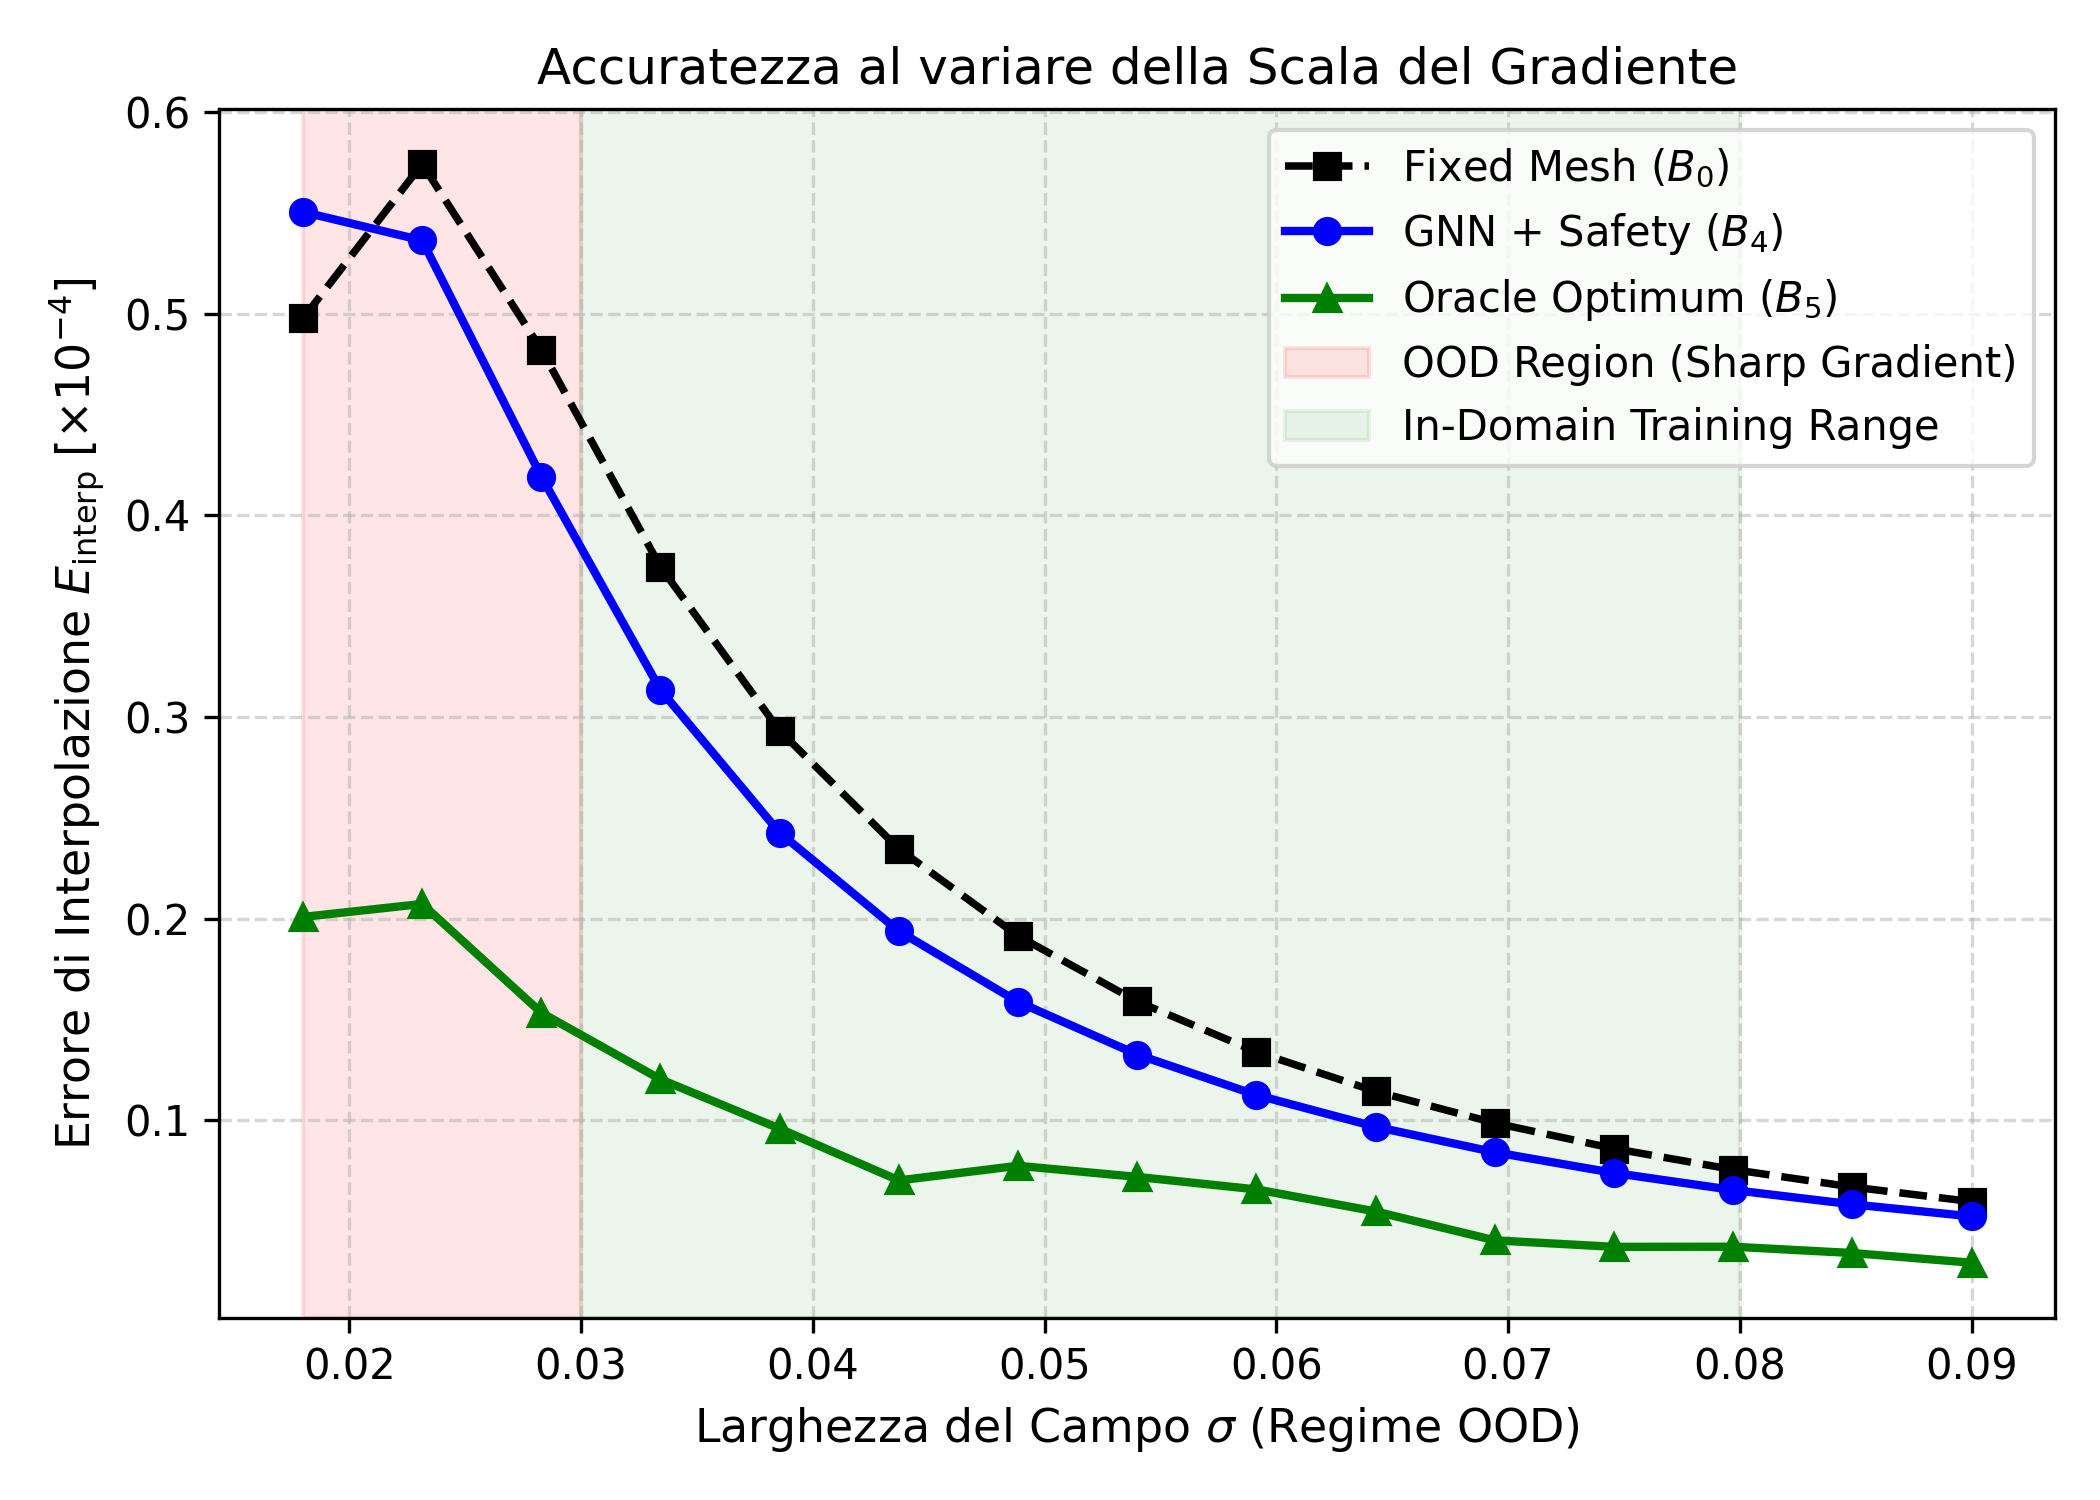
\includegraphics[width=0.95\linewidth]
    {images/stage_a/fig1_error_vs_ood.png}
    \caption{Errore di interpolazione della mesh fissa, della GNN e della configurazione di riferimento sui test interpolativo ed extrapolativo dello Stage A.}
    \label{fig:stage_a_error}
\end{figure}

\begin{figure}[H]
    \centering
    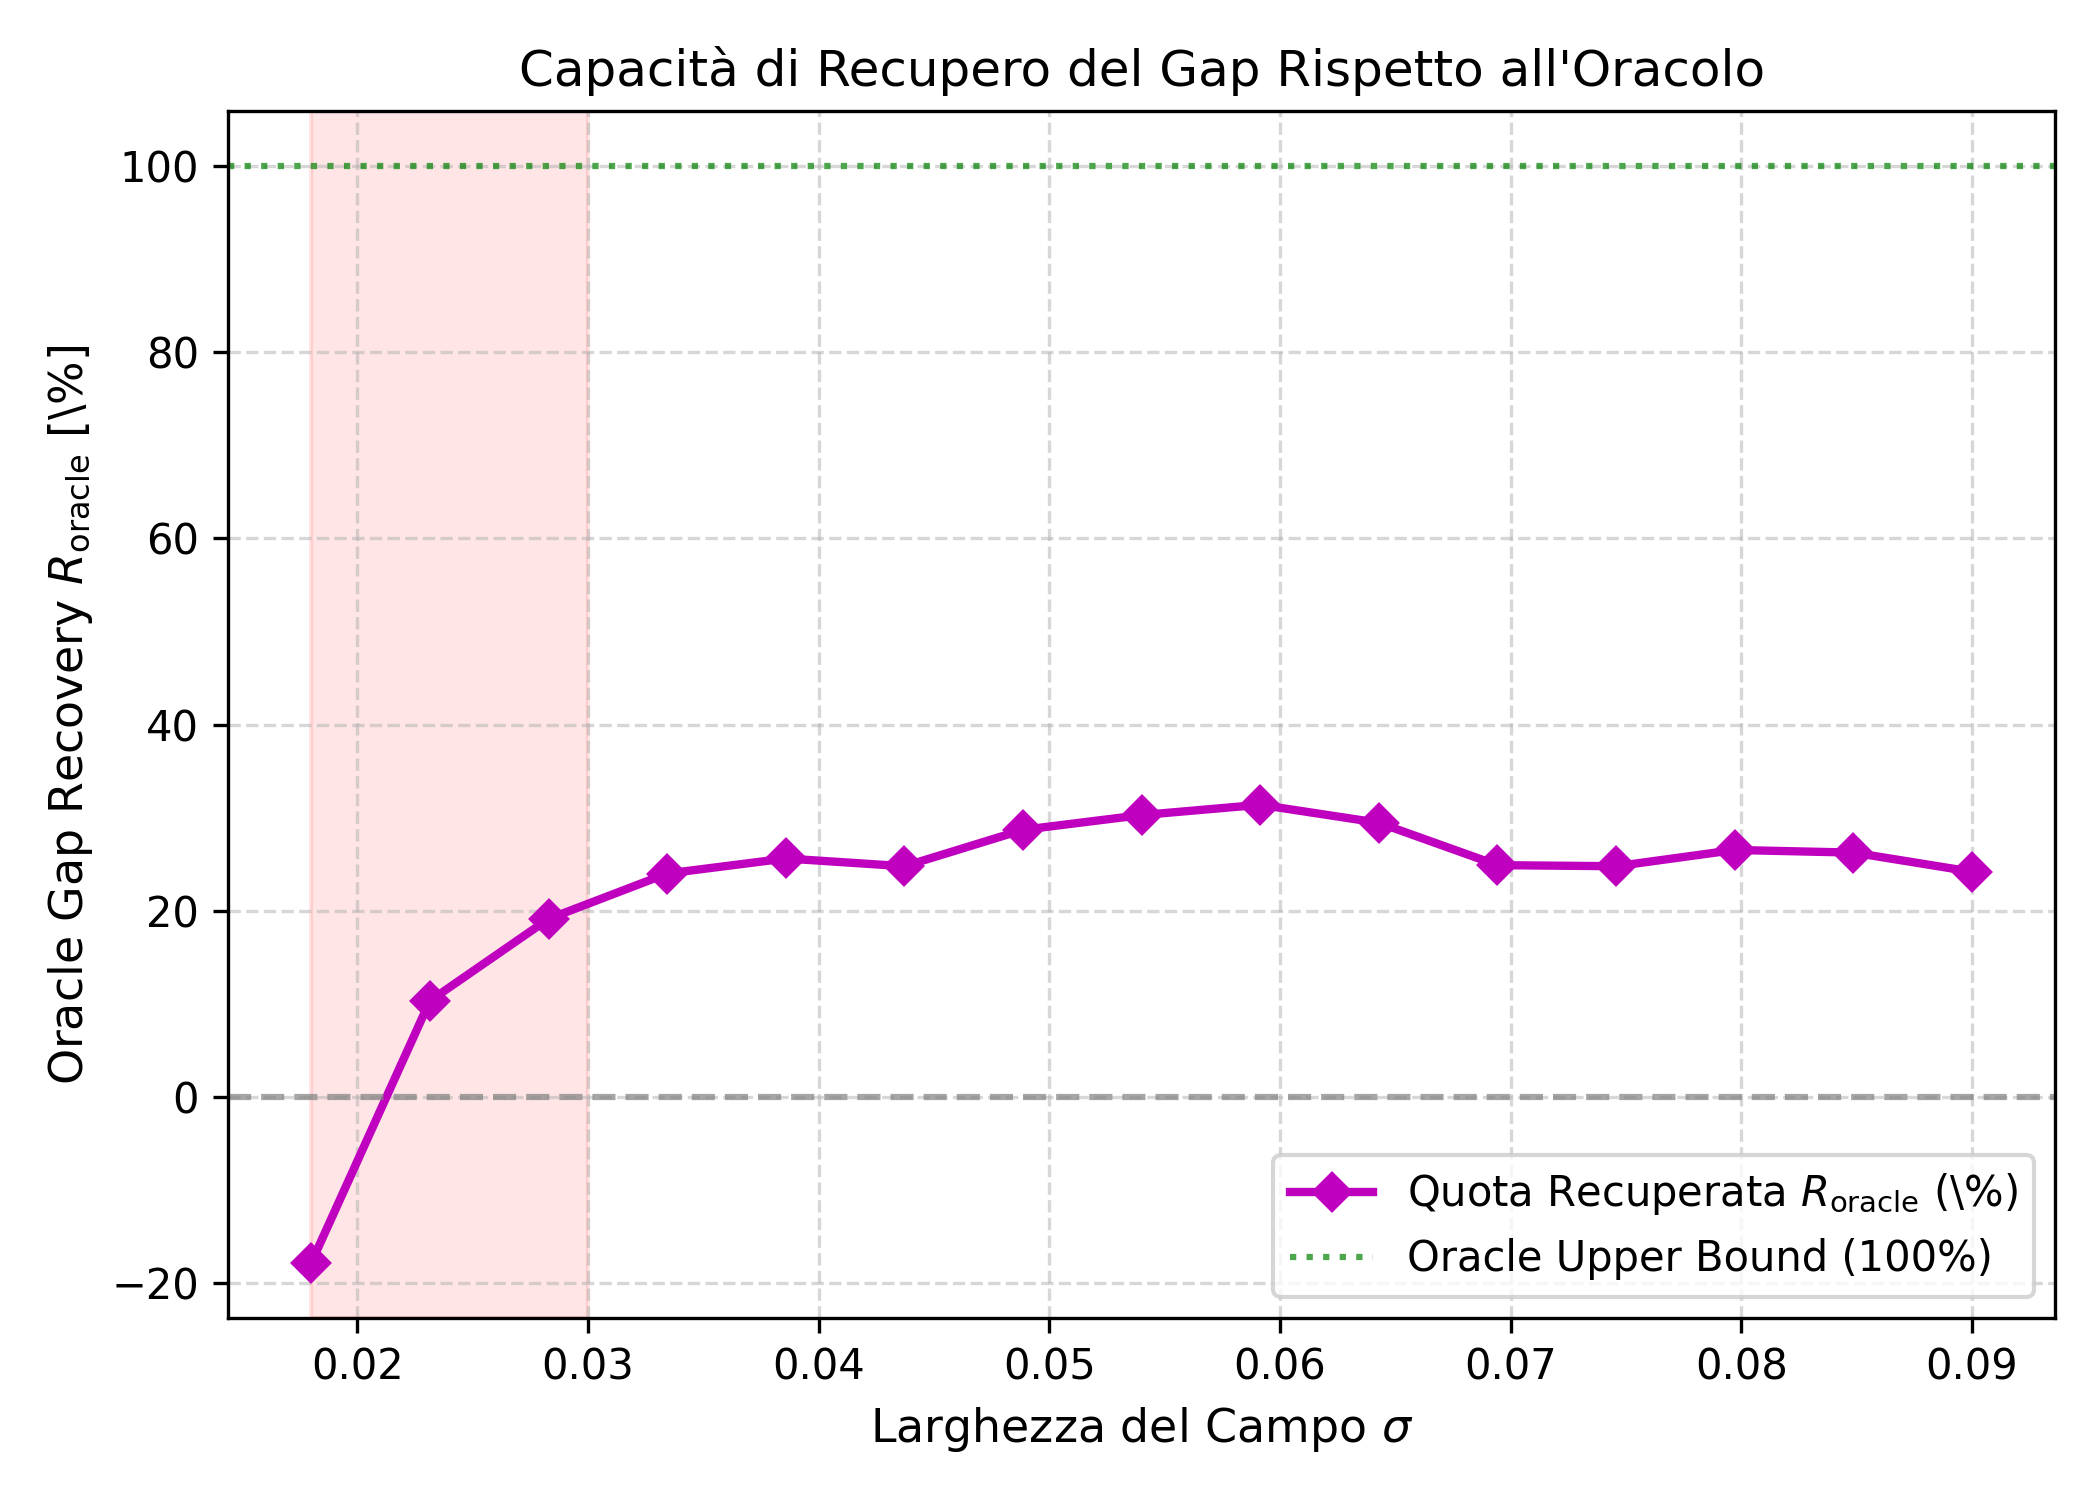
\includegraphics[width=0.85\linewidth]
    {images/stage_a/fig2_oracle_recovery.png}
    \caption{Recupero del divario rispetto all'oracolo ottenuto dalla GNN nei due regimi di test.}
    \label{fig:stage_a_oracle_gap}
\end{figure}

\paragraph{Verifica deterministica del Safety Filter.}

La validazione del filtro viene condotta separatamente dal benchmark principale attraverso uno stress test nel quale lo spostamento prodotto dalla GNN viene moltiplicato per un fattore

\[
k\in\{1,\;1.5,\;2,\;3,\;5,\;10\}.
\]

Per $k\leq3$ la deformazione rimane ammissibile senza alcuna contrazione. Per $k=5$ e $k=10$, invece, la configurazione non filtrata contiene elementi con determinante Jacobiano negativo.

Per $k=5$ il minimo Jacobiano non filtrato scende a

\[
-3.45\times10^{-4},
\]

mentre il Safety Filter determina

\[
\alpha_{\mathrm{global}}\simeq0.678
\]

e porta la configurazione filtrata a una soglia minima pari, entro l'accuratezza numerica del calcolo, a

\[
\min_e J_e \simeq 10^{-4}.
\]

Nel caso più severo, $k=10$, il minimo Jacobiano non filtrato raggiunge

\[
-1.85\times10^{-3},
\]

mentre il fattore ammissibile viene ridotto a

\[
\alpha_{\mathrm{global}}\simeq0.339,
\]

con

\[
\min_e J_e \simeq 10^{-4}.
\]

Il test mostra quindi due comportamenti distinti: per deformazioni già ammissibili il filtro risulta trasparente, mentre per deformazioni che violano il vincolo geometrico riduce automaticamente l'ampiezza dello spostamento fino alla soglia ammissibile. La proprietà è verificata nel modello geometrico considerato, ossia triangoli lineari, traiettoria nodale lineare e soglia prescritta.

\begin{figure}[H]
    \centering
    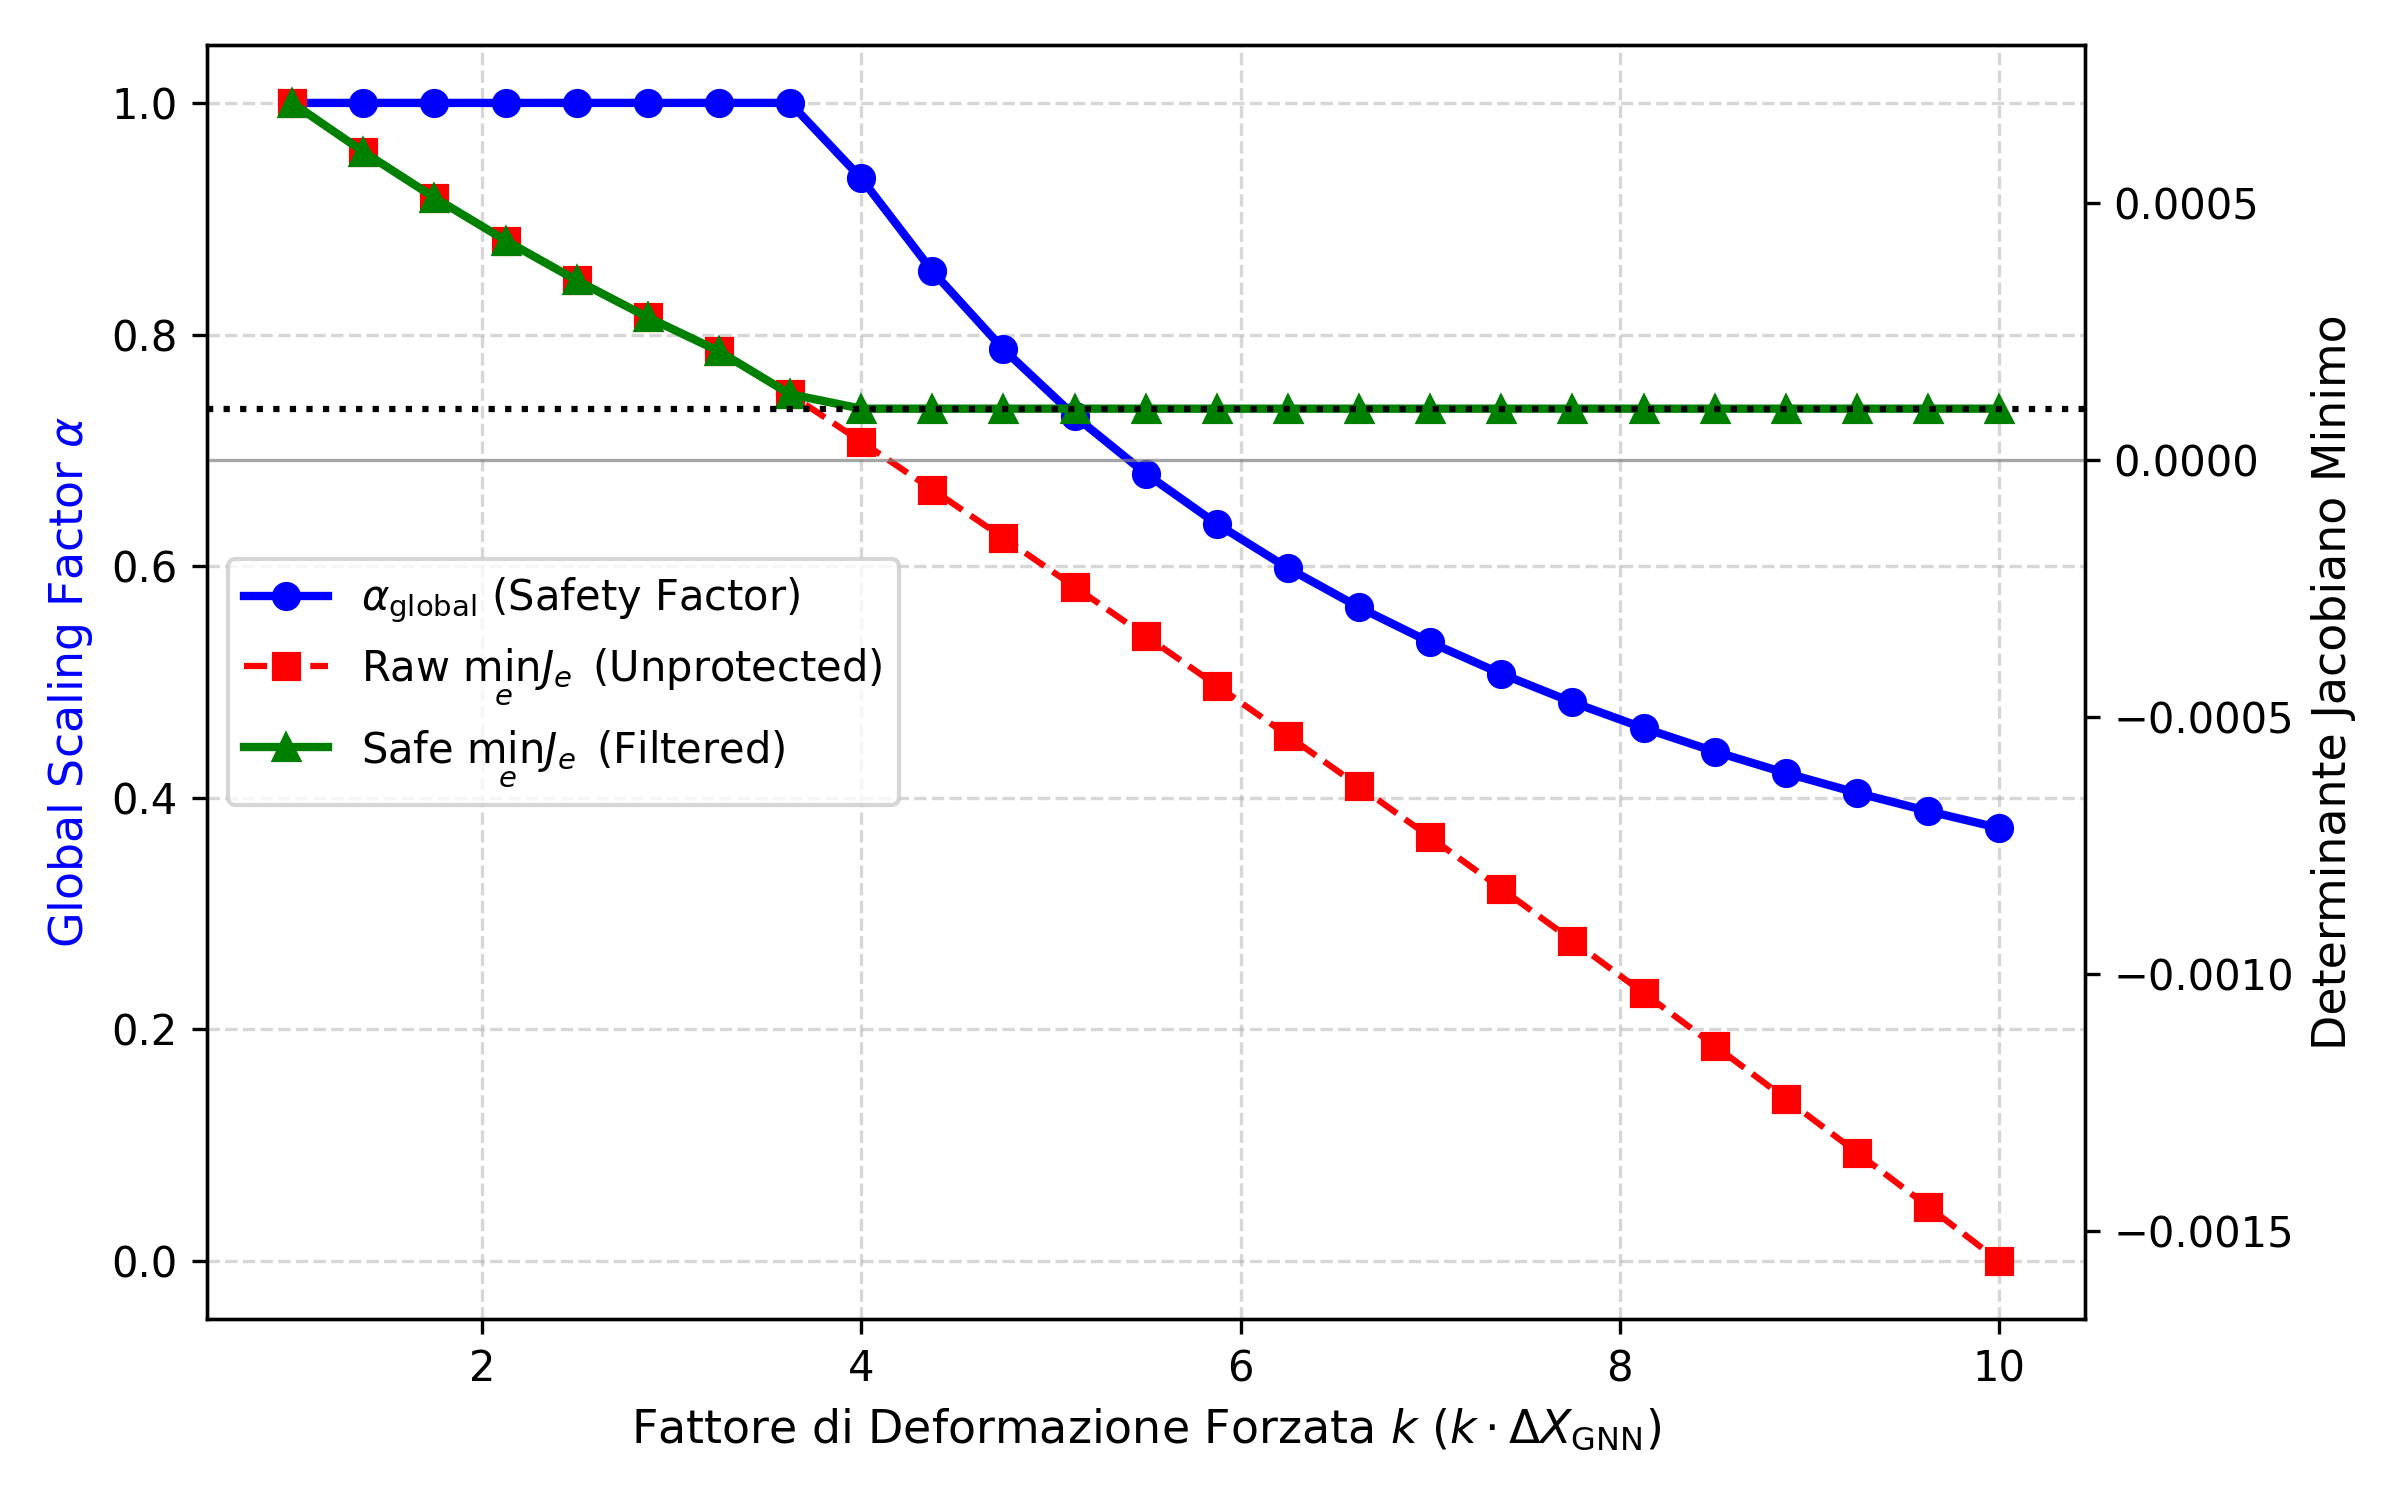
\includegraphics[width=0.85\linewidth]
    {images/stage_a/fig3_safety_curve.png}
    \caption{Attivazione del Safety Filter durante lo stress test geometrico al crescere dell'ampiezza dello spostamento.}
    \label{fig:stage_a_safety}
\end{figure}

La verifica visiva della deformazione prima e dopo il filtraggio è riportata nella Figura~\ref{fig:stage_a_safety_visual}.

\begin{figure}[H]
    \centering
    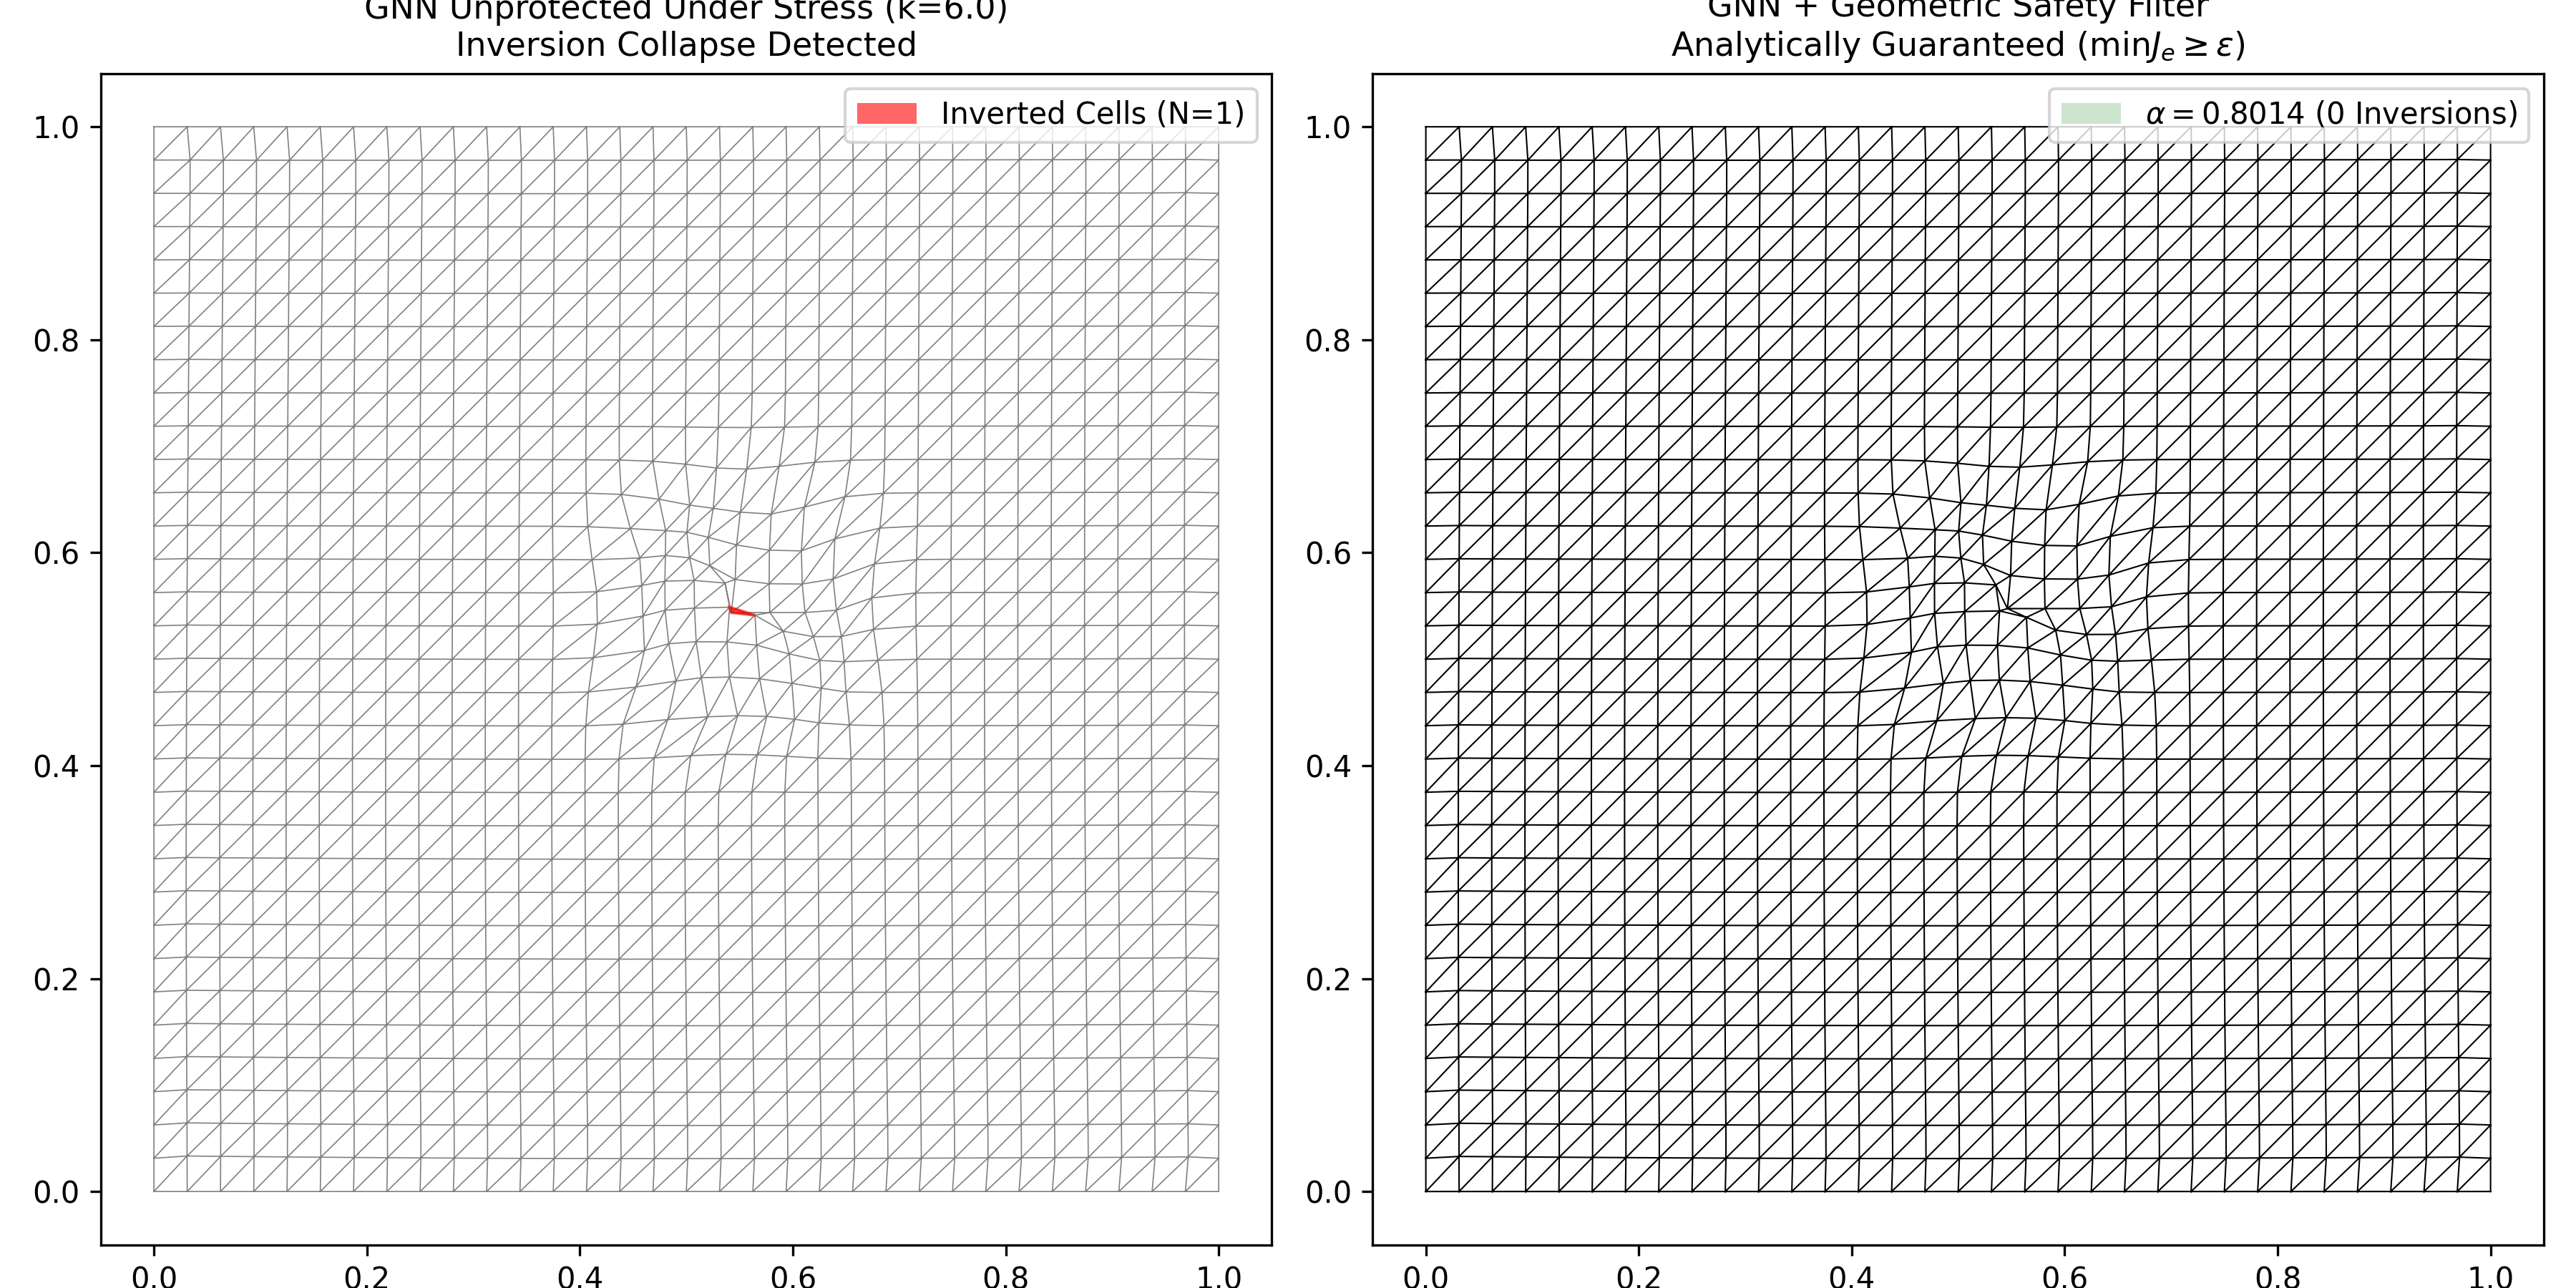
\includegraphics[width=0.95\linewidth]
    {images/stage_a/vis2_safety_stress_visual.png}
    \caption{Esempio di configurazione deformata nello stress test e correzione ottenuta mediante il Safety Filter.}
    \label{fig:stage_a_safety_visual}
\end{figure}

\paragraph{Costo computazionale e scaling.}

Il costo delle tre componenti principali viene misurato utilizzando esclusivamente CPU, così da rendere coerente il confronto tra inferenza GNN, Safety Filter e ottimizzazione variazionale. Il benchmark considera mesh comprese tra $289$ e $4225$ nodi.

Il tempo di inferenza GNN cresce da $15.19$ ms a $184.79$ ms, mentre il costo del Safety Filter passa da $0.23$ ms a $1.39$ ms. L'oracolo variazionale cresce invece da $1.02$ s fino a circa $95.17$ s.

Un fit di potenza sui punti misurati fornisce uno scaling empirico approssimativamente pari a

\[
T_{\mathrm{GNN}}\propto N^{0.93},
\qquad
T_{\mathrm{oracle}}\propto N^{1.69}.
\]

Tali esponenti devono essere interpretati esclusivamente come osservazioni empiriche sul range di dimensioni considerato e non come stime della complessità asintotica generale dei due algoritmi.

\begin{figure}[H]
    \centering
    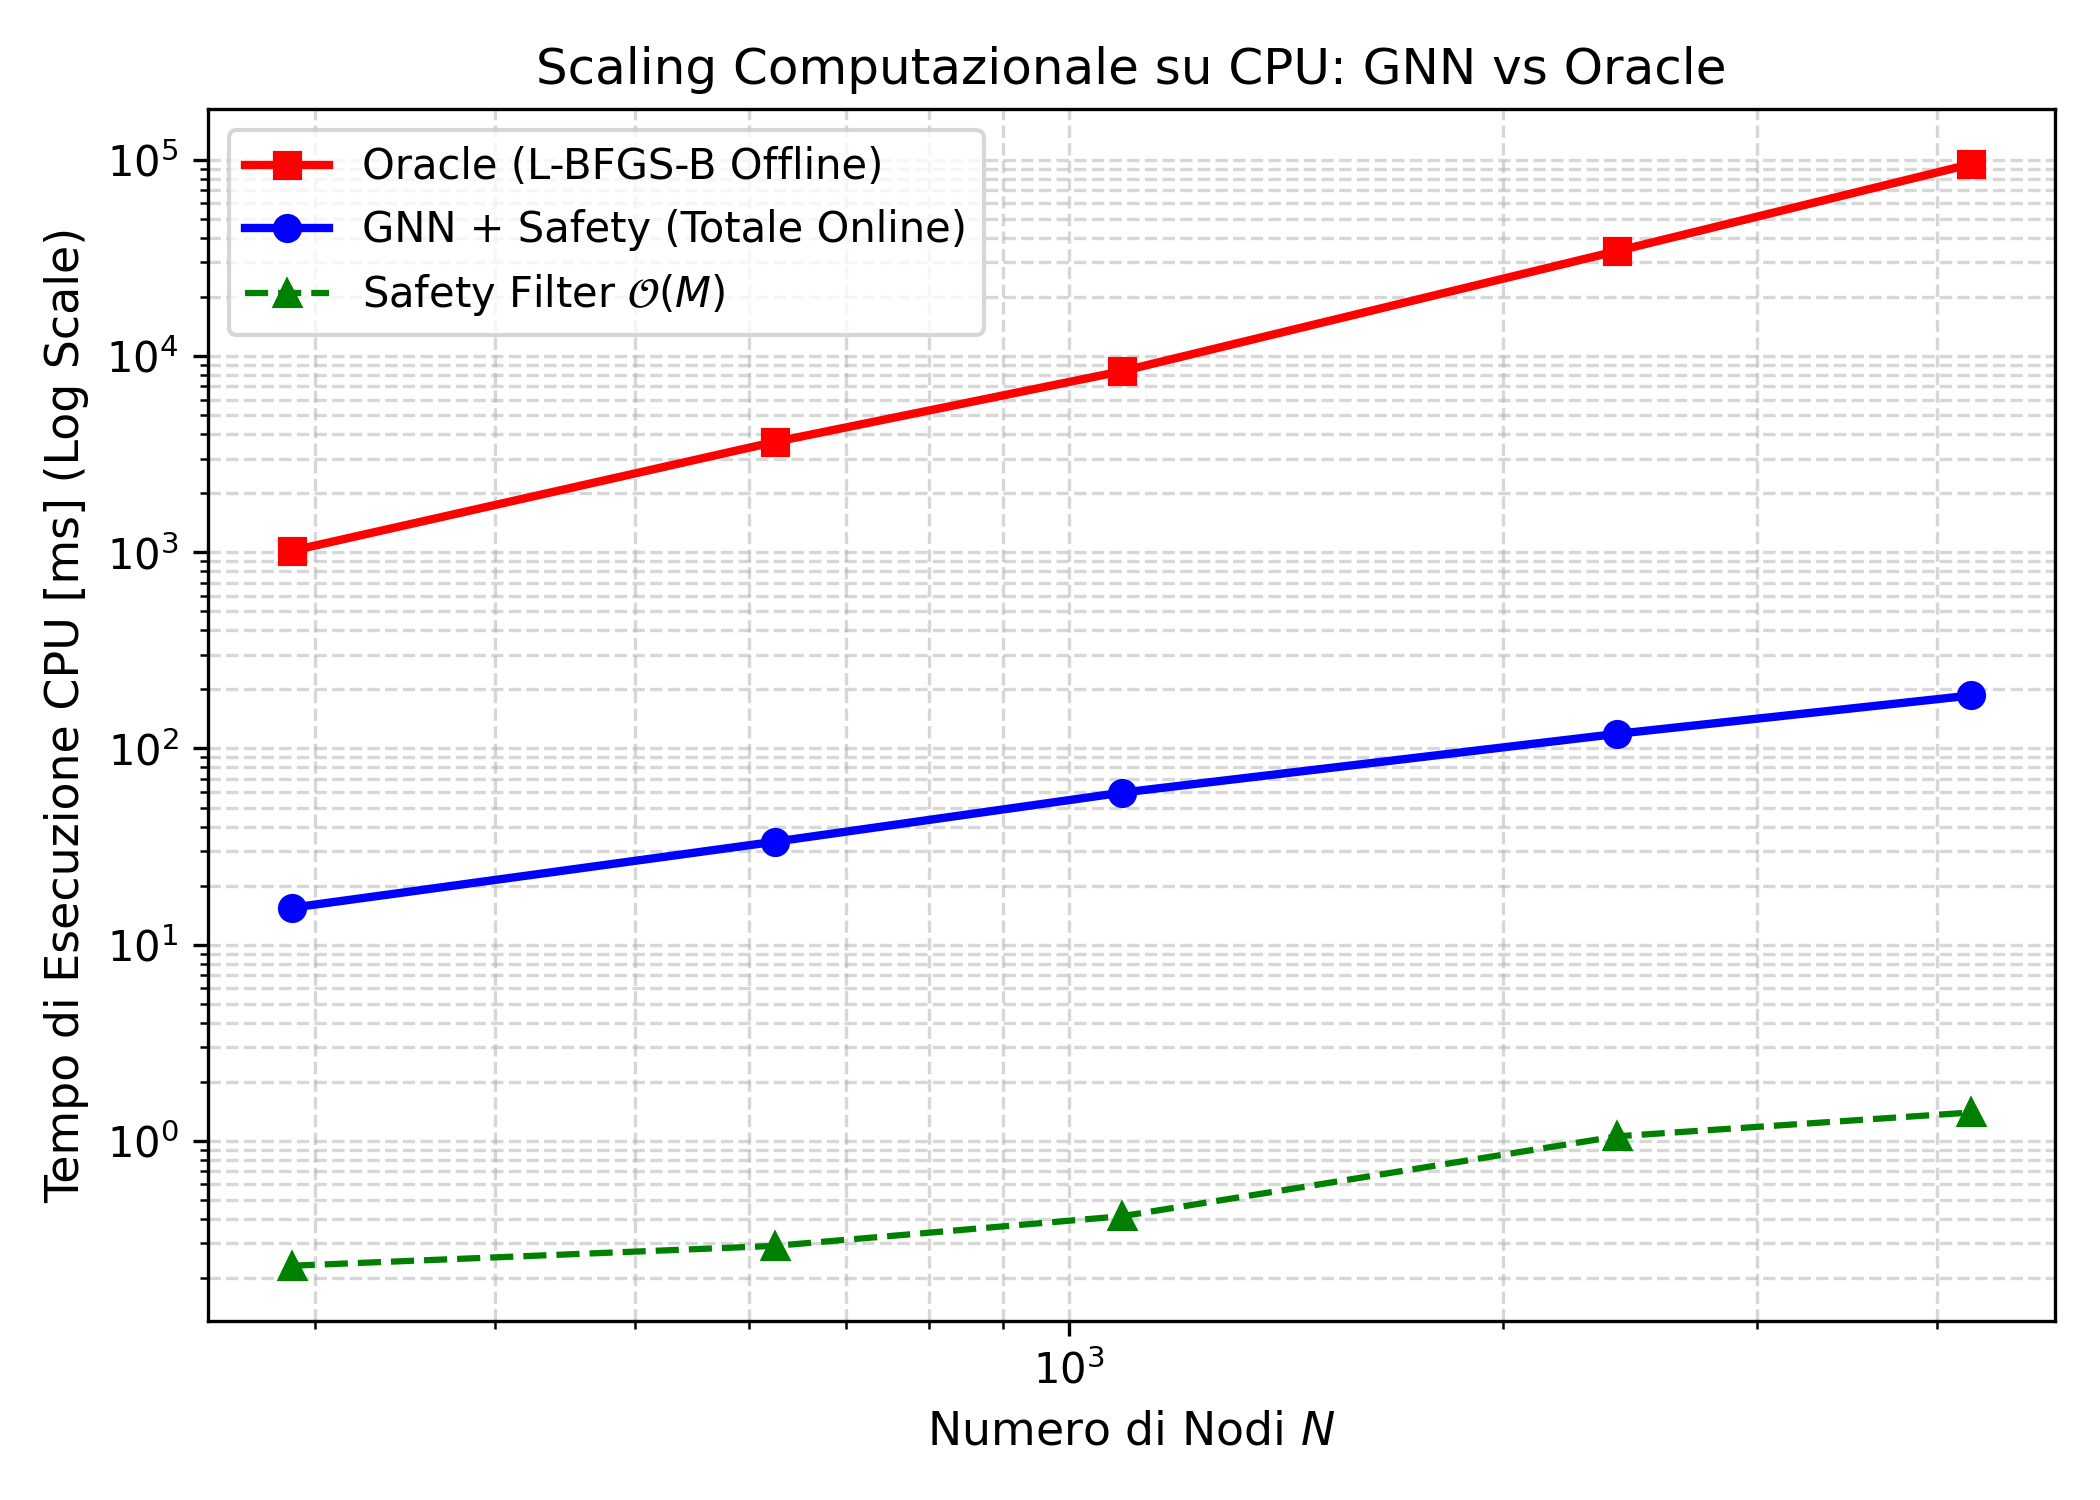
\includegraphics[width=0.90\linewidth]
    {images/stage_a/fig4_runtime_scaling.png}
    \caption{Scaling empirico del costo di inferenza GNN, Safety Filter e ottimizzazione variazionale nello Stage A.}
    \label{fig:stage_a_runtime}
\end{figure}

Nel complesso, lo Stage A mostra che il mesh mover neurale recupera una parte misurabile del beneficio geometrico dell'oracolo e che il controllo geometrico deterministico ha un costo computazionale molto inferiore all'ottimizzazione variazionale nel range di dimensioni testato.

\subsection{Diagnostica dinamica disaccoppiata: Stage B}

\label{subsec:stage_b_diagnostics}

Lo Stage B introduce l'evoluzione temporale della PDE di convezione--diffusione definita nella Sezione~\ref{subsec:pde_governing}. L'obiettivo non è ancora confrontare end-to-end le differenti strategie di mesh motion, ma quantificare separatamente l'impatto del trasferimento dello stato numerico e verificare il comportamento del solutore FEM prima dell'introduzione della formulazione ALE.

La validazione viene pertanto suddivisa in tre gruppi di test:

\begin{enumerate}
    \item verifica indipendente del solutore FEM su mesh fissa;
    \item caratterizzazione del remapping pointwise $P_1$ e della proiezione globale $L^2$;
    \item integrazione della GNN nel problema transiente e studio della frequenza di adattamento.
\end{enumerate}

\subsubsection{Verifica del solutore FEM}

Prima di introdurre il movimento della mesh viene verificata la convergenza del solutore sulla configurazione fissa. Il raffinamento spaziale restituisce ordini di convergenza in norma $L^2$ pari a

\[
1.71,\qquad1.89,\qquad1.97,
\]

mentre per la norma $H^1$ si ottengono

\[
0.80,\qquad0.92,\qquad0.98.
\]

Analogamente, il raffinamento temporale con Backward Euler restituisce ordini

\[
1.04,\qquad1.09,\qquad1.22.
\]

I risultati sono compatibili con gli ordini attesi della discretizzazione $P_1$--Backward Euler discussi nella Sezione~\ref{subsec:fem_discretization}. La verifica stabilisce pertanto che il solutore di riferimento riproduce il comportamento di convergenza previsto prima dell'introduzione del moto della mesh.

\subsubsection{Diagnostica degli operatori di remapping}

La prima verifica riguarda l'esattezza su campi semplici. La proiezione $L^2$ riproduce un campo costante e un campo lineare con errori massimi dell'ordine di

\[
10^{-15},
\]

coerentemente con l'esattezza dello spazio $P_1$ per tali funzioni nel test numerico considerato.

Il successivo studio di convergenza spaziale mostra che entrambi gli operatori convergono al raffinamento della mesh, ma con comportamenti quantitativamente differenti. Per il remapping pointwise $P_1$ vengono osservati ordini sperimentali pari a circa

\[
1.96,\qquad2.00,\qquad2.01,
\]

mentre la proiezione $L^2$ presenta gli ordini

\[
4.12,\qquad2.76,\qquad2.28.
\]

Questi valori sono interpretati esclusivamente come ordini osservati nel benchmark. In particolare, il valore iniziale superiore a $4$ non viene assunto come indicazione di un ordine teorico globale della proiezione $L^2$; l'ultima finestra di raffinamento fornisce un valore pari a $2.28$.

Un secondo test varia l'ampiezza dello spostamento della mesh. Per i fattori di deformazione

\[
\gamma=\{0.1,0.25,0.5,1,2\},
\]

l'errore relativo del remapping pointwise passa da circa $0.20\%$ a $2.96\%$, mentre quello della proiezione $L^2$ rimane compreso tra circa $0.01\%$ e $0.26\%$.

Il test di accumulo a target finale fisso costituisce il confronto più diretto tra i due operatori. Dividendo lo stesso spostamento complessivo in $K=\{1,2,5,10\}$ trasferimenti successivi, il remapping $P_1$ produce errori finali pari a

\[
4.220\%,\quad
5.235\%,\quad
5.779\%,\quad
5.949\%,
\]

con fattori di amplificazione rispettivamente pari a

\[
1.00,\quad1.24,\quad1.37,\quad1.41.
\]

La proiezione $L^2$ produce invece

\[
0.172\%,\quad
0.160\%,\quad
0.364\%,\quad
0.332\%,
\]

con fattori di amplificazione

\[
1.00,\quad0.93,\quad2.12,\quad1.93.
\]

I risultati mostrano che l'applicazione reiterata dell'interpolazione pointwise può produrre un accumulo di errore sensibilmente superiore rispetto alla proiezione globale nel test considerato. La proiezione $L^2$ non elimina tuttavia completamente l'errore introdotto dal trasferimento: i valori misurati rimangono infatti finiti e dipendono dalla configurazione geometrica e dalla frequenza delle proiezioni.

La differenza in accuratezza è accompagnata da un incremento del costo computazionale. Sulla mesh $32\times32$ il tempo medio misurato è circa

\[
27.02\ {\rm ms}
\]

per il remapping $P_1$ e

\[
355.55\ {\rm ms}
\]

per la proiezione $L^2$, corrispondente a un rapporto di costo di circa

\[
13.2\times.
\]

Questa evidenza motiva il passaggio alla formulazione ALE dello Stage C: il problema non consiste soltanto nella scelta del trasferimento più accurato, ma anche nella necessità di eliminare, quando possibile, un'operazione di trasferimento separata che viene ripetuta durante l'evoluzione temporale.

\begin{figure}[H]
    \centering
    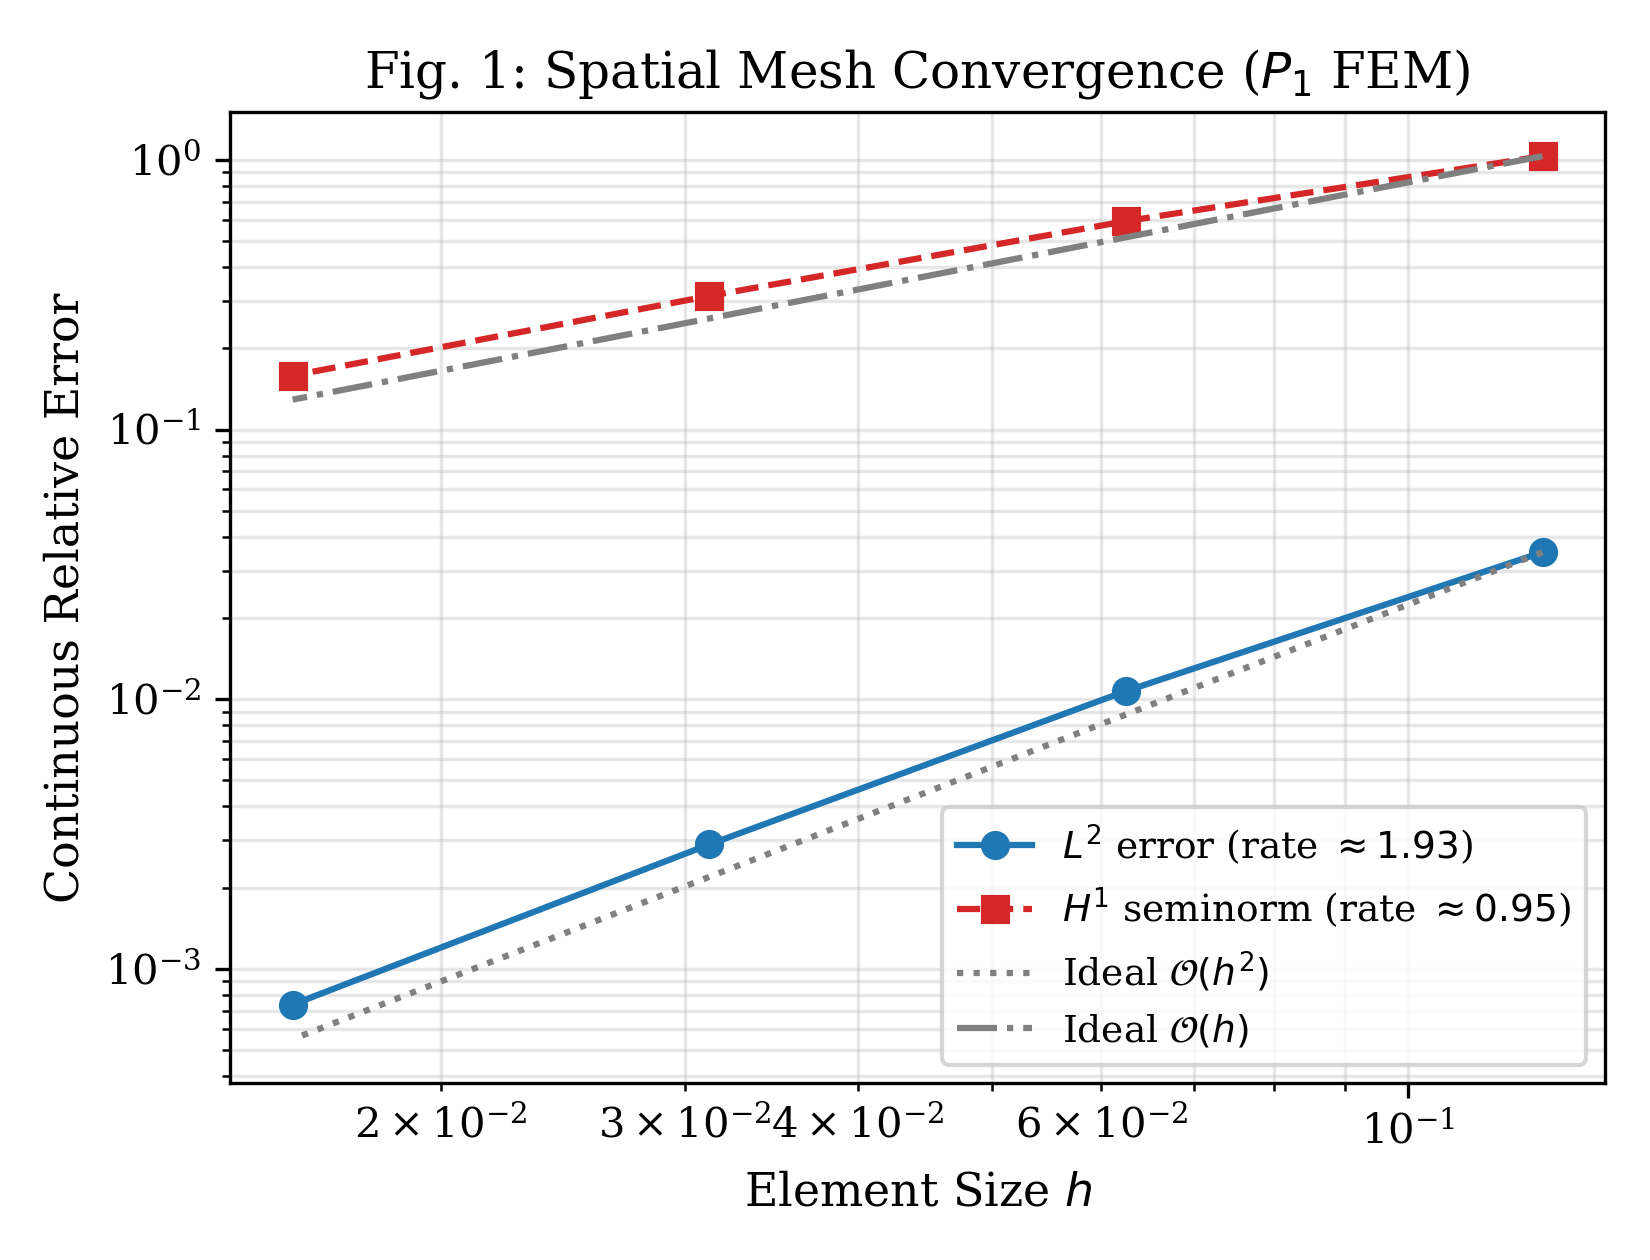
\includegraphics[width=0.90\linewidth]
    {images/stage_b/fig1_spatial_convergence.png}
    \caption{Convergenza spaziale del solutore FEM e confronto tra remapping pointwise $P_1$ e proiezione $L^2$.}
    \label{fig:stage_b_spatial}
\end{figure}

\begin{figure}[H]
    \centering
    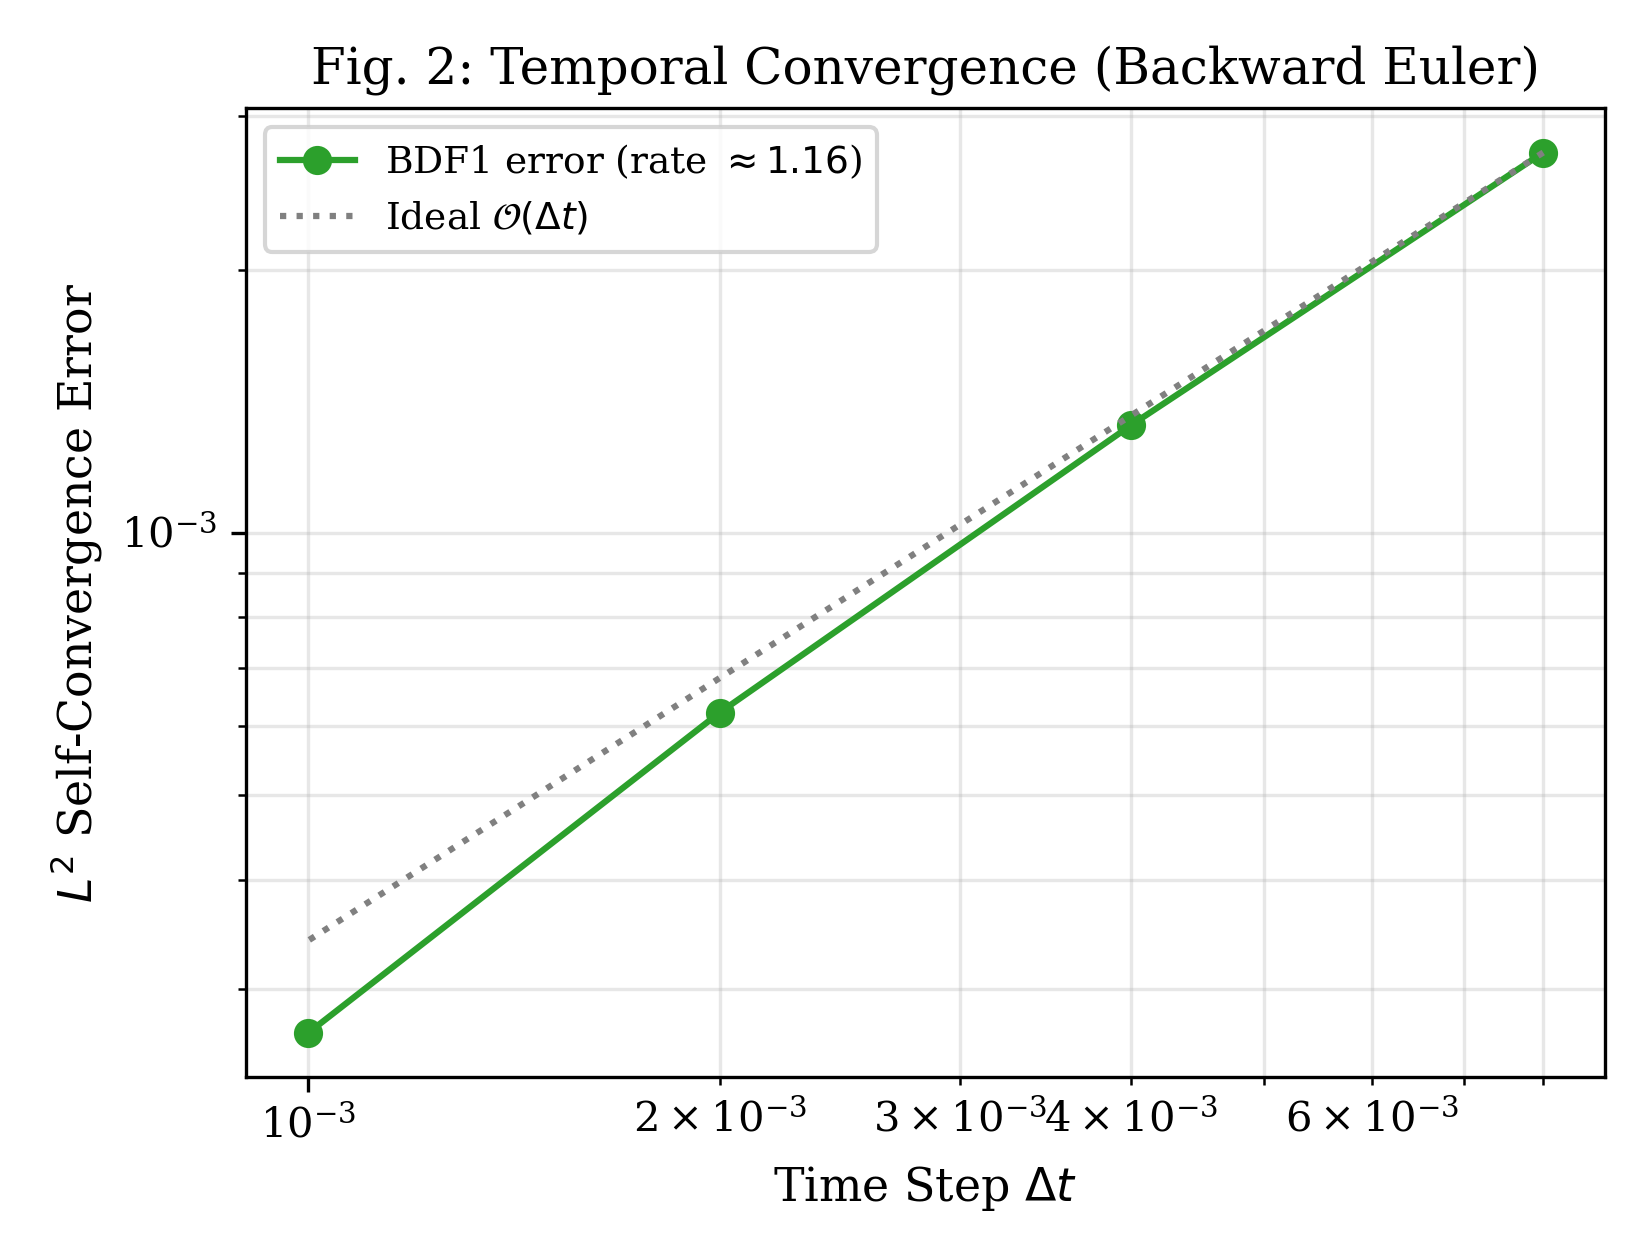
\includegraphics[width=0.90\linewidth]
    {images/stage_b/fig2_temporal_convergence.png}
    \caption{Convergenza temporale del solutore Backward Euler nello Stage B.}
    \label{fig:stage_b_temporal}
\end{figure}

\subsubsection{Diagnostica dell'accoppiamento GNN--PDE e dell'impatto del trasferimento di stato}

Dopo aver isolato il comportamento degli operatori su singoli eventi di trasferimento, viene valutato l'impatto dell'accumulo dell'errore durante l'evoluzione transiente della PDE descritta nella Sezione~\ref{subsec:pde_governing}. Questa campagna diagnostica non costituisce il benchmark comparativo finale dell'intero framework, ma mira a rispondere a una domanda metodologica specifica: l'errore aggiuntivo osservato con mesh mobile è associato principalmente alla configurazione geometrica prodotta dalla GNN oppure al meccanismo di trasferimento dello stato?

A tale scopo vengono confrontate la discretizzazione su mesh fissa e tre configurazioni dinamiche con intervallo di adattamento $N_a=10$ passi temporali, caratterizzate da differenti meccanismi di trasferimento.

\begin{table}[htbp]
\centering
\small
\setlength{\tabcolsep}{6pt}
\caption{Diagnostica dello Stage B: confronto dell'accuratezza PDE al tempo finale $T=0.5$ e dell'errore integrato nel tempo.}
\label{tab:stage_b_main}
\begin{tabular*}{\linewidth}{@{\extracolsep{\fill}}lcc@{}}
\toprule
Configurazione di verifica & $E_{L^2}(T)$ & $\overline{E}_{L^2}$ (time-integrated) \\
\midrule
Mesh fissa (riferimento Euleriano)  & $9.03\%$ & $7.96\%$ \\
GNN + remapping pointwise $P_1$    & $12.72\%$ & $10.32\%$ \\
GNN + proiezione $L^2$              & $8.99\%$ & $7.89\%$ \\
Oracle istantaneo + proiezione $L^2$ & $9.57\%$ & $8.35\%$ \\
\bottomrule
\end{tabular*}
\end{table}

La configurazione GNN + $P_1$ mostra un errore finale maggiore della mesh fissa, coerentemente con i risultati della diagnostica del trasferimento. Sostituendo il remapping pointwise con la proiezione $L^2$, l'errore finale scende a $8.99\%$, mentre l'errore integrato nel tempo risulta pari a $7.89\%$.

Nel benchmark considerato, lo scostamento rispetto alla mesh fissa rimane quindi contenuto. Il risultato più rilevante dello Stage B è la forte riduzione dell'errore aggiuntivo associato al trasferimento pointwise quando questo viene sostituito dalla proiezione $L^2$, a fronte del corrispondente incremento di costo computazionale.

Anche l'oracolo, quando accoppiato alla stessa proiezione $L^2$, restituisce un errore finale del $9.57\%$. Questo risultato conferma che l'oracolo introdotto nello Stage A deve essere interpretato come riferimento per la qualità geometrica istantanea e non come soluzione ottima del problema PDE transiente.

\paragraph{Gradiente FEM rispetto al gradiente analitico.}

Per verificare se la qualità dell'informazione fornita alla GNN dipenda in modo significativo dalla disponibilità della soluzione analitica, viene confrontato l'utilizzo del gradiente calcolato dal solutore FEM con quello analitico esatto.

La configurazione con gradiente FEM produce

\[
8.989\%
\]

di errore finale e

\[
7.890\%
\]

di errore integrato nel tempo, mentre il gradiente analitico produce rispettivamente

\[
8.979\%
\]

e

\[
7.889\%.
\]

La differenza è quindi molto ridotta nel benchmark considerato. Il risultato supporta l'impiego del gradiente FEM disponibile durante la simulazione come feature operativa della GNN, senza richiedere l'accesso alla soluzione analitica nella pipeline dinamica.

\paragraph{Sensibilità alla frequenza di adattamento.}

La frequenza di aggiornamento della mesh determina un compromesso tra accuratezza e costo computazionale. Considerando intervalli di adattamento pari a $5$, $10$, $20$ e $50$ passi temporali, si ottengono i risultati riportati in Tabella~\ref{tab:stage_b_frequency}.

\begin{table}[htbp]
\centering
\footnotesize
\setlength{\tabcolsep}{3pt}
\caption{Sensibilità dello Stage B alla frequenza di adattamento.}
\label{tab:stage_b_frequency}
\begin{tabular*}{\linewidth}{@{\extracolsep{\fill}}ccccc@{}}
\toprule
\begin{tabular}[c]{@{}c@{}}Intervallo\\ $N_a$\end{tabular} &
\begin{tabular}[c]{@{}c@{}}Adatt.\\ totali\end{tabular} &
\begin{tabular}[c]{@{}c@{}}Errore\\ $L^2(T)$\end{tabular} &
\begin{tabular}[c]{@{}c@{}}Errore\\ integrato\end{tabular} &
\begin{tabular}[c]{@{}c@{}}Tempo\\ tot. [s]\end{tabular} \\
\midrule
$5$  & $20$ & $8.984\%$ & $7.819\%$ & $9.50$ \\
$10$ & $10$ & $8.989\%$ & $7.890\%$ & $5.25$ \\
$20$ & $5$  & $9.001\%$ & $7.932\%$ & $3.11$ \\
$50$ & $2$  & $9.039\%$ & $7.957\%$ & $1.82$ \\
\bottomrule
\end{tabular*}
\end{table}

La riduzione della frequenza di adattamento diminuisce progressivamente il costo della simulazione, mentre l'errore varia solo moderatamente nel range considerato. Nel benchmark esaminato, l'aggiornamento della mesh a ogni passo temporale non risulta quindi necessario per mantenere un livello di accuratezza comparabile, introducendo un ulteriore parametro di controllo del costo della strategia adattiva.

\begin{figure}[H]
    \centering
    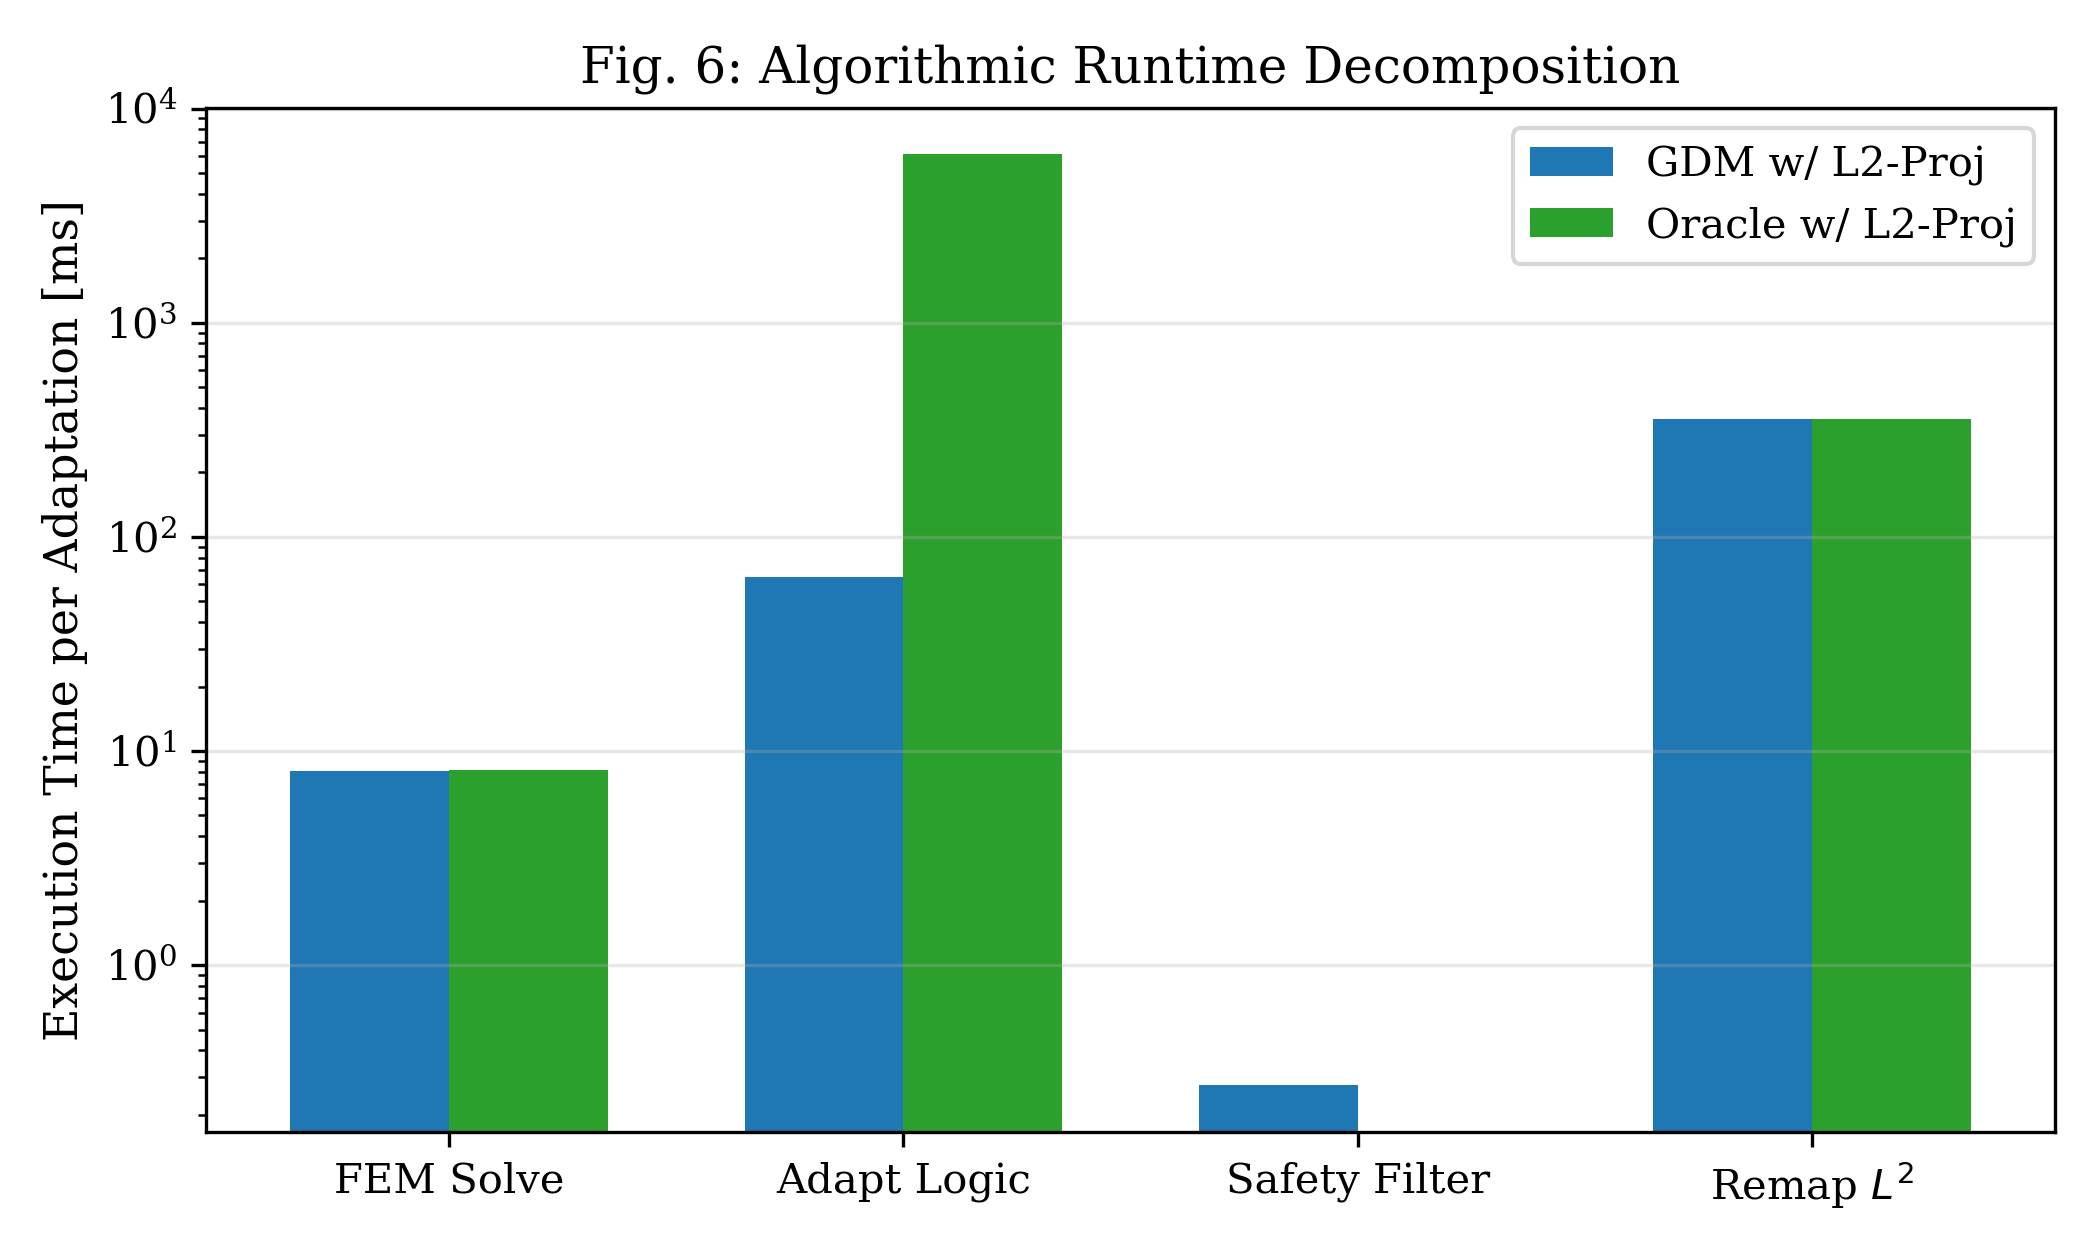
\includegraphics[width=0.95\linewidth]
    {images/stage_b/fig6_runtime_decomposition.png}
    \caption{Scomposizione del costo computazionale della simulazione dinamica nello Stage B.}
    \label{fig:stage_b_runtime}
\end{figure}

\begin{figure}[H]
    \centering
    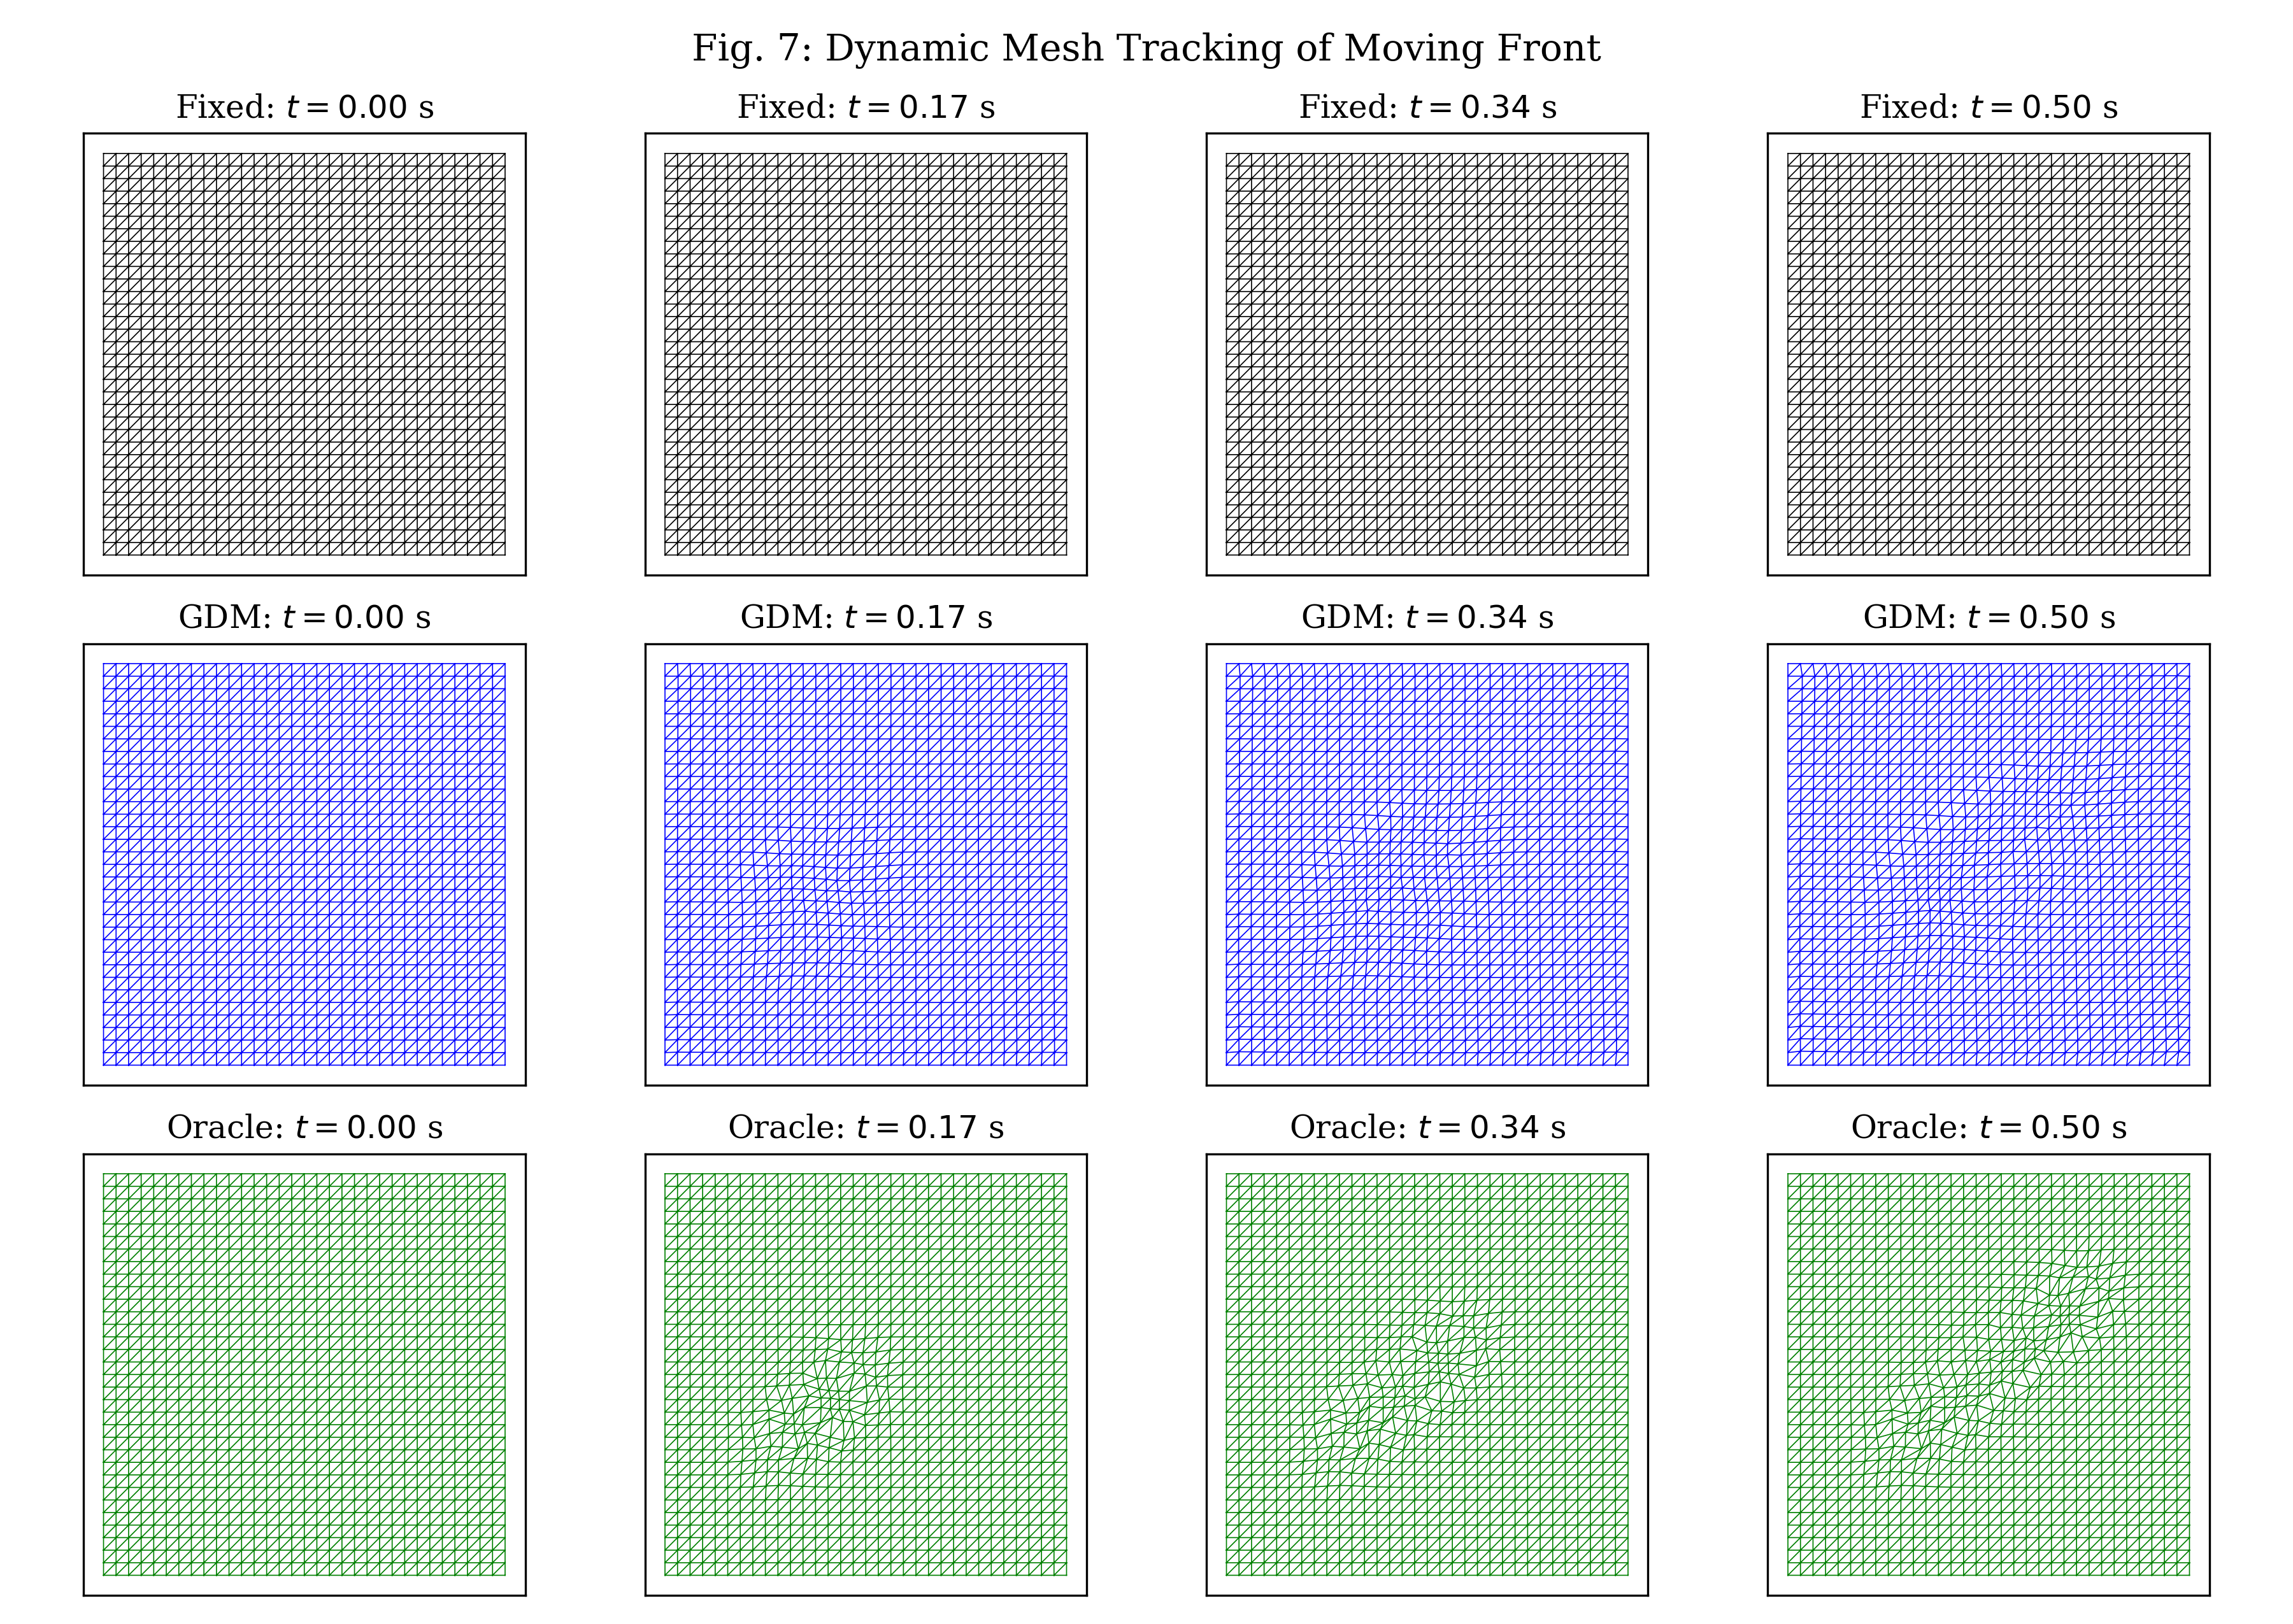
\includegraphics[width=0.95\linewidth]
    {images/stage_b/fig7_qualitative_dynamic_mesh.png}
    \caption{Evoluzione qualitativa della mesh adattata durante la simulazione transiente.}
    \label{fig:stage_b_mesh}
\end{figure}

\begin{figure}[H]
    \centering
    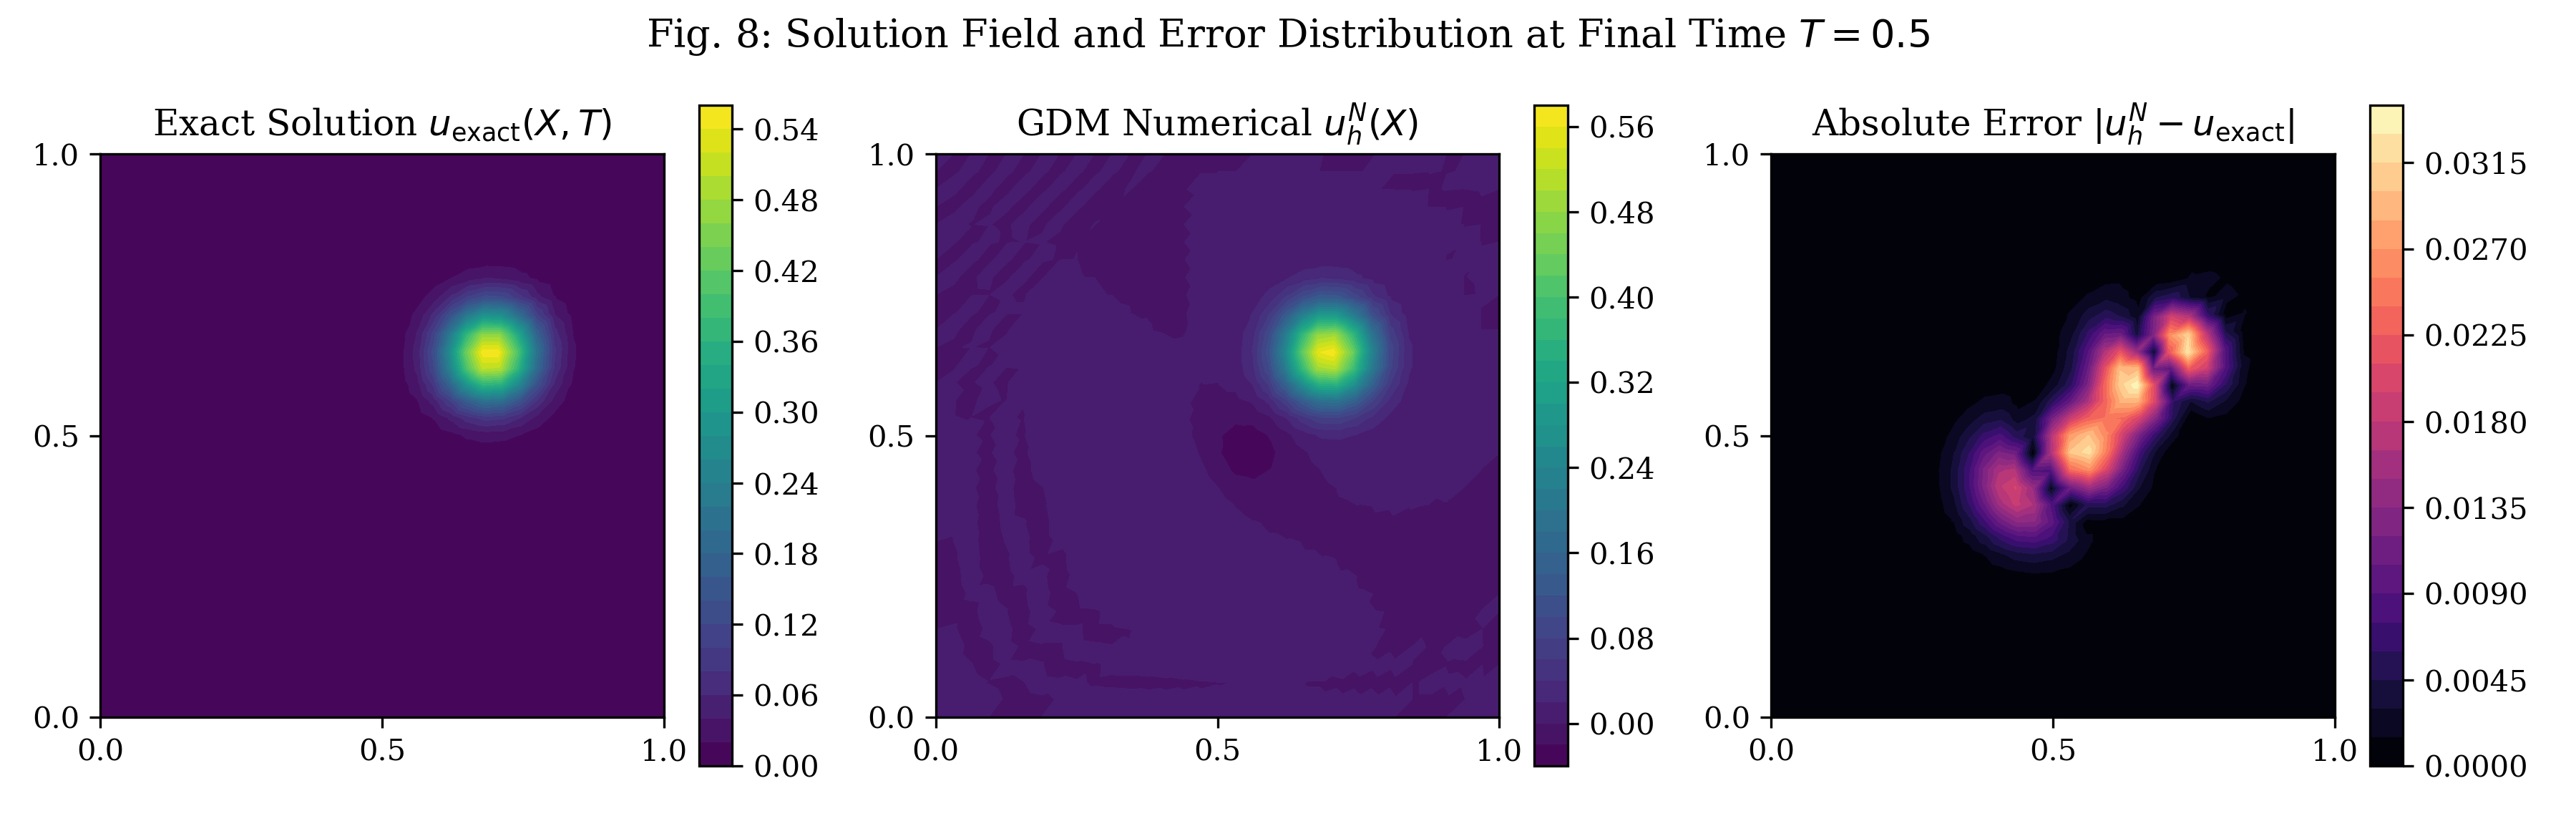
\includegraphics[width=0.90\linewidth]
    {images/stage_b/fig8_pde_error_field.png}
    \caption{Distribuzione spaziale dell'errore PDE nello Stage B.}
    \label{fig:stage_b_error_field}
\end{figure}

\paragraph{Conclusioni dello Stage B.}

Lo Stage B mostra che l'accuratezza globale di una simulazione a mesh mobile non può essere attribuita esclusivamente alla qualità della configurazione geometrica. Il trasferimento dello stato costituisce una componente numerica indipendente e può diventare rilevante quando viene ripetuto durante l'evoluzione temporale.

La proiezione $L^2$ riduce in modo significativo l'errore associato al trasferimento rispetto al remapping pointwise nel benchmark considerato, ma introduce un costo computazionale sensibilmente maggiore. Questa evidenza motiva il passaggio a una formulazione nella quale il moto della mesh viene incorporato direttamente nell'equazione differenziale.

\subsection{Verifica ALE e D-GCL: Stage C}

\label{subsec:stage_c_verification}

Lo Stage C introduce la formulazione ALE descritta nella Sezione~\ref{subsec:ale_formulation}. A differenza dello Stage B, nel quale ogni aggiornamento discreto della mesh richiede un trasferimento esplicito dello stato, lo spostamento prodotto dalla GNN viene distribuito su una finestra temporale e trasformato in una velocità di mesh continua a tratti.

Prima di utilizzare la formulazione ALE nel benchmark dinamico finale, vengono eseguiti cinque test indipendenti, indicati come C1--C5. Tali test verificano separatamente la cinematica della mesh, la consistenza geometrica, l'effetto della deformazione sulla soluzione PDE e il mantenimento degli ordini di convergenza spaziale e temporale.

\subsubsection{Test C1: verifica cinematica della velocità di mesh}

\label{subsubsec:c1}

Il primo test verifica la corrispondenza tra lo spostamento nodale prescritto e la velocità discreta

\[
\mathbf{w}^{n+\frac12}
=
\frac{\mathbf{X}^{n+1}-\mathbf{X}^{n}}{\Delta t}.
\]

Nel test considerato, l'errore relativo $L^2$ sulla velocità di mesh è

\[
1.64\times10^{-4},
\]

mentre l'errore $L^\infty$ è

\[
3.97\times10^{-5}.
\]

Il risultato mostra che la discretizzazione cinematica utilizzata dal solutore ALE rappresenta con errore contenuto il movimento nodale imposto.

\subsubsection{Test C2: verifica della D-GCL e preservazione del free stream}

\label{subsubsec:c2}

La consistenza geometrica discreta dello schema ALE viene verificata mediante gli indicatori introdotti nella Sezione~\ref{subsec:dgcl} su una sequenza di $100$ passi temporali deformanti.

Il massimo residuo geometrico element-wise risulta

\[
\max_{n,e}R_e^{\mathrm{GCL}}
=
4.34\times10^{-17},
\]

mentre il residuo della relazione matriciale discreta risulta

\[
\max_n
R_{\mathrm{alg}}^{\mathrm{GCL}}
=
5.42\times10^{-17}.
\]

Entrambi i valori sono prossimi alla precisione di macchina e indicano una forte consistenza numerica tra la variazione geometrica degli elementi e la discretizzazione della velocità di mesh.

La verifica del free stream, ottenuta imponendo un campo costante $u_0\equiv1$, fornisce

\[
E_{\mathrm{FS}}
=
2.81\times10^{-14}.
\]

Il campo uniforme rimane quindi invariato entro un errore prossimo alla precisione numerica del calcolo.

Nel complesso, i tre indicatori forniscono una verifica indipendente e coerente della D-GCL per la discretizzazione considerata. Il risultato viene interpretato come soddisfacimento della consistenza geometrica entro la precisione numerica osservata; non viene invece utilizzato come prova di una proprietà generale di conservazione fisica della PDE.

\subsubsection{Test C3: consistenza a singolo passo mediante MMS}

\label{subsubsec:c3}

Il test C3 confronta la soluzione ottenuta mediante un singolo passo su mesh fissa con quella ottenuta sulla configurazione deformata mediante il solutore ALE.

L'errore relativo $L^2$ risulta pari a

\[
4.0011\%
\]

per il caso di riferimento e

\[
4.1505\%
\]

per la configurazione ALE deformata.

La differenza è quindi pari a circa

\[
0.149
\]

punti percentuali.

Nel singolo passo considerato, la deformazione della mesh introduce pertanto un incremento limitato dell'errore complessivo rispetto alla configurazione fissa.

\begin{figure}[H]
    \centering
    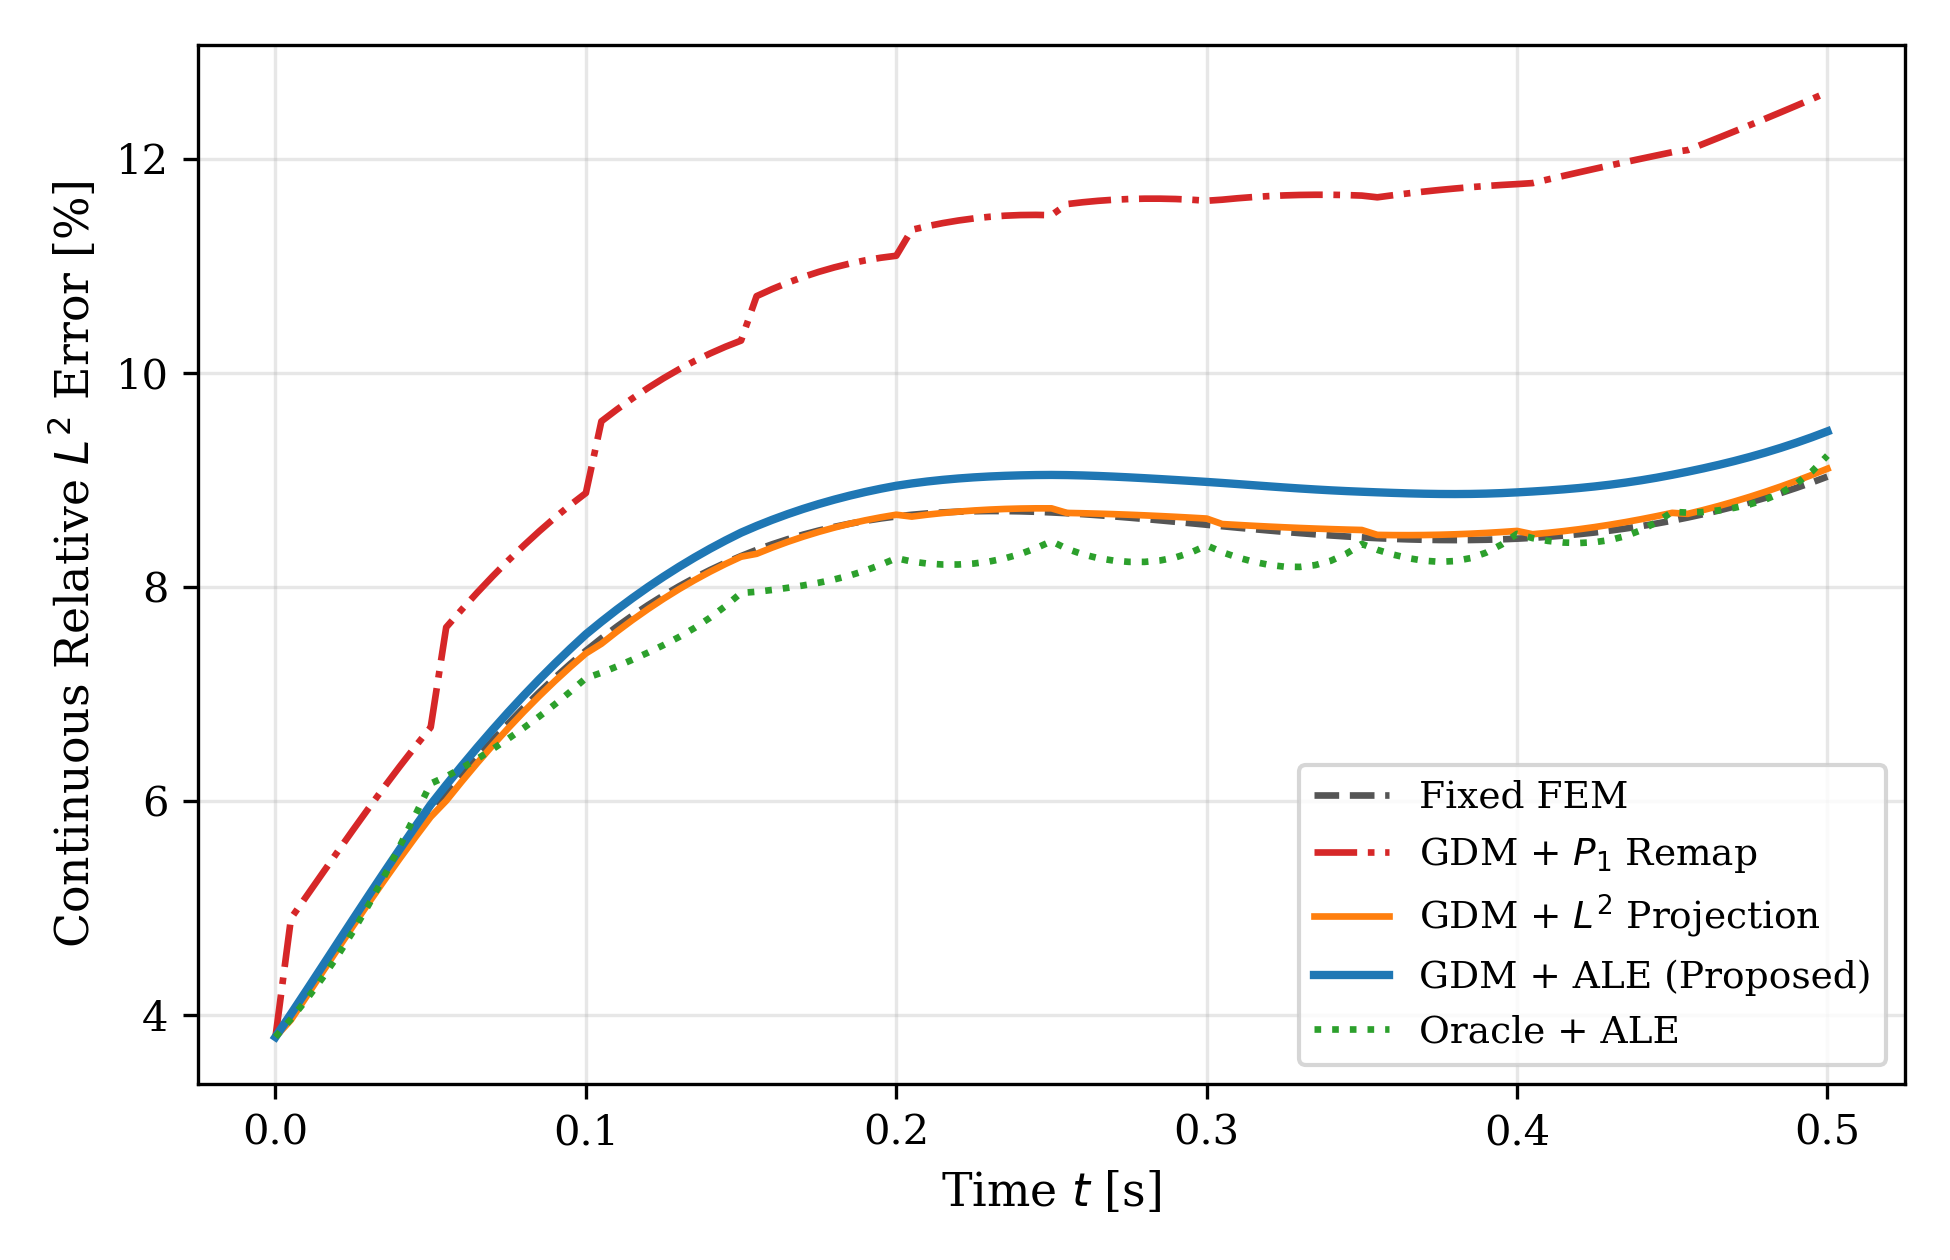
\includegraphics[width=0.90\linewidth]
    {images/stage_c/fig_c3_dynamic_error.png}
    \caption{Confronto dell'errore PDE nel test C3 tra configurazione fissa e configurazione ALE deformata.}
    \label{fig:stage_c_c3}
\end{figure}

\subsubsection{Test C4: convergenza spaziale su mesh deformate}

\label{subsubsec:c4}

Il test C4 verifica il comportamento della discretizzazione spaziale in presenza di mesh deformate, mantenendo la stessa topologia e aumentando progressivamente la risoluzione della griglia. L'errore viene misurato nelle norme $L^2$ e $H^1$ rispetto alla soluzione manufactured.

Per le risoluzioni considerate si ottengono i valori riportati in Tabella~\ref{tab:stage_c_spatial_convergence}.

\begin{table}[htbp]
\centering
\small
\setlength{\tabcolsep}{5pt}
\caption{Convergenza spaziale del solutore ALE su mesh deformate.}
\label{tab:stage_c_spatial_convergence}
\begin{tabular}{ccccc}
\toprule
Mesh & $E_{L^2}$ & Rate $L^2$ & $E_{H^1}$ & Rate $H^1$ \\
\midrule
$8\times8$   & $3.7062\times10^{-1}$ & --   & $7.1340\times10^{-1}$ & --   \\
$16\times16$ & $1.4345\times10^{-1}$ & $1.37$ & $4.5983\times10^{-1}$ & $0.63$ \\
$32\times32$ & $3.8812\times10^{-2}$ & $1.89$ & $2.4297\times10^{-1}$ & $0.92$ \\
$64\times64$ & $9.9228\times10^{-3}$ & $1.97$ & $1.2323\times10^{-1}$ & $0.98$ \\
\bottomrule
\end{tabular}
\end{table}

Gli ordini osservati tendono progressivamente ai valori attesi per elementi lineari $P_1$:

\[
\mathcal{O}(h^2)
\qquad\text{in }L^2,
\]

e

\[
\mathcal{O}(h)
\qquad\text{in }H^1.
\]

In particolare, sulle due ultime finestre di raffinamento vengono osservati ordini pari a $1.89$ e $1.97$ in norma $L^2$, e $0.92$ e $0.98$ in norma $H^1$. Il comportamento indica che la deformazione della mesh non impedisce il recupero del regime asintotico atteso nel range di risoluzioni considerato.

\subsubsection{Test C5: convergenza temporale per auto-convergenza}

\label{subsubsec:c5}

La convergenza temporale viene verificata mediante un test di auto-convergenza di tipo Cauchy utilizzando tre valori del passo temporale:

\[
\Delta t
=
0.01,\quad
0.005,\quad
0.0025.
\]

Le differenze tra soluzioni a passi successivi sono rispettivamente

\[
6.4654\times10^{-3},
\qquad
3.2591\times10^{-3},
\qquad
1.6482\times10^{-3},
\]

con ordini sperimentali pari a

\[
0.99
\qquad\text{e}\qquad
0.98.
\]

Il comportamento osservato è quindi compatibile con il primo ordine temporale atteso per Backward Euler,

\[
\mathcal{O}(\Delta t).
\]

\subsubsection{Sintesi della validazione Stage C}

Nel loro insieme, i test C1--C5 verificano separatamente le proprietà necessarie prima dell'introduzione della formulazione ALE nel benchmark dinamico finale:

\begin{itemize}
    \item C1 verifica la correttezza cinematica della velocità di mesh;
    \item C2 verifica la D-GCL elementare e algebrica e la preservazione del free stream;
    \item C3 quantifica l'effetto immediato della deformazione sulla soluzione PDE;
    \item C4 verifica il recupero degli ordini spaziali attesi della discretizzazione $P_1$ su mesh deformate;
    \item C5 verifica il primo ordine temporale della discretizzazione Backward Euler.
\end{itemize}

Nel complesso, i test mostrano che il solutore ALE conserva, nel regime esaminato, il comportamento di consistenza e convergenza della discretizzazione di riferimento anche in presenza di mesh deformate.

\paragraph{Sintesi complessiva della validazione.}

La sequenza Stage A--C permette di isolare progressivamente tre livelli del problema. Lo Stage A verifica che la GNN possa produrre deformazioni utili e che tali deformazioni possano essere sottoposte a un controllo geometrico deterministico. Lo Stage B mostra che, una volta inserito il movimento in una simulazione PDE transiente, il trasferimento dello stato costituisce una sorgente indipendente di errore e costo. Lo Stage C verifica quindi che il passaggio a una descrizione ALE continua sia compatibile con la discretizzazione FEM, con la D-GCL e con gli ordini di convergenza osservati.

Il significato dei tre stadi è quindi distinto: lo Stage A valuta la capacità di adattamento geometrico, lo Stage B quantifica il compromesso tra accuratezza e costo dei differenti operatori di trasferimento, mentre lo Stage C verifica la consistenza della formulazione ALE prima del confronto end-to-end.

Il confronto finale tra la strategia basata sulla proiezione $L^2$ e quella basata sulla formulazione ALE viene pertanto demandato al benchmark dinamico del capitolo successivo, dove le diverse pipeline vengono valutate con metriche comuni di accuratezza, costo computazionale e robustezza geometrica.

\newpage

% =============================================================
% 6. RISULTATI DINAMICI E BENCHMARK COMPARATIVO
% =============================================================
\section{Transient Dynamic Benchmark and Comparative Analysis}
\label{sec:dynamic_benchmark}
Dopo aver verificato separatamente i singoli componenti metodologici, il presente capitolo considera la pipeline GDM nella sua configurazione completa mediante un esperimento dinamico end-to-end. L'obiettivo è valutare il comportamento del framework quando il mesh mover neurale, il \textit{Safety Filter}, il solutore FEM e il meccanismo di evoluzione o trasferimento della mesh operano congiuntamente durante l'integrazione temporale della PDE.

Il confronto finale è organizzato attorno a tre aspetti distinti ma strettamente correlati: accuratezza della soluzione numerica, costo computazionale complessivo e robustezza geometrica della discretizzazione. In particolare, viene confrontato il riferimento a mesh fissa con differenti strategie di gestione della mesh mobile basate sul medesimo modello GNN: il remapping pointwise $P_1$, la proiezione $L^2$ e la formulazione ALE continua. L'obiettivo non è stabilire una superiorità assoluta di una singola configurazione, ma quantificare il compromesso tra accuratezza, costo e gestione della mesh associato ai differenti meccanismi di accoppiamento.

\subsection{Configurazione del benchmark e baseline di confronto}

\label{subsec:benchmark_setup}

La campagna di valutazione dinamica end-to-end adotta la configurazione fisica di convezione--diffusione e la Manufactured Solution analitica $u^\star(\mathbf{x},t)$ definite nella Sezione~\ref{subsec:pde_governing}, operando sul dominio $\Omega=[0,1]^2$ fino all'istante finale $T=0.5$, con

\[
\mathbf{b}=(0.4,0.2)^T,
\qquad
\nu=10^{-3}.
\]

La triangolazione di partenza è uniforme a risoluzione $32\times32$, corrispondente a $N=1089$ nodi e $M=2048$ elementi triangolari $P_1$. L'integrazione temporale utilizza lo schema Backward Euler con passo costante

\[
\Delta t=5\times10^{-3},
\]

su un totale di $100$ passi temporali. L'aggiornamento della configurazione geometrica viene effettuato ogni $N_a=10$ passi.

A ciascun evento di adattamento, la MeshMover GNN riceve lo stato FEM disponibile durante la simulazione e produce uno spostamento nodale. Lo spostamento viene quindi sottoposto al Deterministic Safety Filter, introdotto nella Sezione~\ref{subsec:safety_filter}, che verifica l'ammissibilità della traiettoria lineare della mesh rispetto alla soglia

\[
\epsilon=10^{-4}.
\]

Tale controllo è applicato secondo le ipotesi geometriche definite nel Capitolo~\ref{sec:gdm_framework} e non viene interpretato come una proprietà generale indipendente dalla discretizzazione considerata.

Per il benchmark finale vengono confrontate quattro configurazioni:

\begin{table}[htbp]
\centering
\small
\setlength{\tabcolsep}{3pt}
\caption{Configurazioni considerate nel benchmark dinamico finale.}
\label{tab:final_baselines}
\begin{tabular*}{\linewidth}{@{\extracolsep{\fill}}lcccc@{}}
\toprule
Configurazione &
\begin{tabular}[c]{@{}c@{}}Mesh\\ mobile\end{tabular} &
GNN &
\begin{tabular}[c]{@{}c@{}}Trasferimento\\ dello stato\end{tabular} &
ALE \\
\midrule
Fixed FEM   & No  & No  & --                & No \\
GDM + $P_1$ & Sì  & Sì  & $P_1$ pointwise   & No \\
GDM + $L^2$ & Sì  & Sì  & Proiezione $L^2$  & No \\
GDM + ALE   & Sì  & Sì  & Nessuno           & Sì \\
\bottomrule
\end{tabular*}
\end{table}

La configurazione \textit{Fixed FEM} costituisce il riferimento Euleriano e permette di quantificare l'errore ottenuto senza alcun movimento della mesh. La configurazione \textit{GDM + $P_1$} rappresenta l'accoppiamento con il remapping pointwise barycentrico, già analizzato nelle prove dello Stage B. La configurazione \textit{GDM + $L^2$} sostituisce il trasferimento pointwise con la proiezione globale introdotta nella Sezione~\ref{subsec:l2_projection}. Infine, \textit{GDM + ALE} elimina il trasferimento esplicito dello stato e incorpora il moto della mesh direttamente nella formulazione della PDE attraverso la velocità relativa.

Il modello neurale impiegato è identico per tutte le configurazioni basate sulla GNN e corrisponde al checkpoint addestrato offline nello Stage A, senza fine-tuning specifico per il problema transiente.

Per rendere il confronto tra $L^2$ e ALE il più possibile controllato, viene utilizzata la medesima sequenza temporale di configurazioni geometriche target prodotte dalla GNN. Questo protocollo deve tuttavia essere distinto dalla traiettoria calcolata direttamente durante la campagna dinamica dello Stage B: i target vengono prescritti agli istanti di adattamento e successivamente riutilizzati nel confronto finale. Nel caso $L^2$, la mesh viene portata direttamente alla configurazione target e lo stato viene trasferito mediante proiezione; nel caso ALE, lo stesso spostamento viene distribuito sui successivi $N_a$ passi e trasformato nella velocità di mesh

\[
\mathbf{w}
=
\frac{\Delta\mathbf{X}_{\mathrm{safe}}}
{N_a\Delta t}.
\]

La differenza tra i due protocolli è quindi intenzionale e consente di confrontare principalmente il meccanismo di gestione del moto della mesh, senza introdurre variazioni nel modello neurale o nella sequenza dei target geometrici.

È inoltre importante notare che i valori ottenuti in questo benchmark finale non coincidono necessariamente con quelli riportati nella diagnostica dinamica dello Stage B. In particolare, il protocollo di replay dei target geometrici adottato nel presente capitolo non coincide punto per punto con la traiettoria numerica generata nel corso della precedente campagna dinamica; i risultati devono pertanto essere confrontati all'interno del rispettivo protocollo sperimentale.

\subsection{Accuratezza della PDE ed evoluzione temporale dell'errore}

\label{subsec:error_dynamics}

La prima metrica considerata è l'errore relativo in norma $L^2$ rispetto alla soluzione manufactured,

\begin{equation}
E_{L^2}(t)
=
\frac{
\|u_h(\cdot,t)-u_{\mathrm{exact}}(\cdot,t)\|_{L^2(\Omega)}
}{
\|u_{\mathrm{exact}}(\cdot,t)\|_{L^2(\Omega)}
},
\label{eq:final_l2_error}
\end{equation}

calcolato a ogni passo temporale. Oltre al valore finale $E_{L^2}(T)$, viene considerato l'errore integrato nel tempo,

\begin{equation}
\overline{E}_{L^2}
=
\frac{1}{T}
\int_0^T
E_{L^2}(t)\,dt,
\label{eq:final_integrated_error}
\end{equation}

approssimato numericamente sulla griglia temporale del benchmark.

Il valore finale misura la precisione raggiunta al termine della simulazione, mentre l'errore integrato nel tempo sintetizza il comportamento complessivo della soluzione e permette di evidenziare eventuali perturbazioni associate agli eventi di adattamento.

\begin{table}[htbp]
\centering
\caption{Accuratezza globale nel benchmark dinamico finale. I valori sono espressi come percentuale dell'errore relativo $L^2$.}
\label{tab:final_accuracy}
\begin{tabular}{lcc}
\toprule
Configurazione
& $E_{L^2}(T)$ [\%]
& $\overline{E}_{L^2}$ [\%]
\\
\midrule
Fixed FEM
& 9.03
& 7.96
\\
GDM + $P_1$
& 12.72
& 10.32
\\
GDM + $L^2$
& 8.92
& 7.87
\\
GDM + ALE
& 9.47
& 8.27
\\
\bottomrule
\end{tabular}
\end{table}

Il confronto mostra innanzitutto una differenza netta tra i due meccanismi di trasferimento esplicito considerati. La configurazione GDM + $P_1$ raggiunge un errore finale del $12.72\%$ e un errore integrato del $10.32\%$, superiori ai corrispondenti valori della mesh fissa. Il risultato è coerente con la diagnostica dello Stage B, nella quale l'applicazione reiterata del remapping pointwise aveva evidenziato un accumulo dell'errore di trasferimento.

La sostituzione del remapping pointwise con la proiezione $L^2$ porta invece a un errore finale dell'$8.92\%$ e a un errore integrato del $7.87\%$. Nel protocollo considerato, questi valori risultano molto vicini a quelli della mesh fissa, con una differenza rispettivamente di circa $0.11$ e $0.09$ punti percentuali. Il risultato indica che la proiezione globale riduce il contributo del trasferimento osservato con il remapping pointwise, senza tuttavia implicare che il movimento della mesh renda in generale la discretizzazione più accurata della baseline fissa.

La formulazione GDM + ALE raggiunge invece un errore finale del $9.47\%$ e un errore integrato dell'$8.27\%$. Rispetto alla proiezione $L^2$, lo scostamento è pari a circa $0.55$ punti percentuali sul valore finale e $0.40$ punti percentuali sul valore integrato. In questo benchmark, quindi, la formulazione ALE conserva un livello di accuratezza comparabile ma leggermente inferiore a quello ottenuto con la proiezione $L^2$.

L'evoluzione temporale dell'errore riportata in Figura~\ref{fig:final_error_dynamics} permette di osservare ulteriormente la differenza tra le strategie di accoppiamento.

\begin{figure}[htbp]
\centering
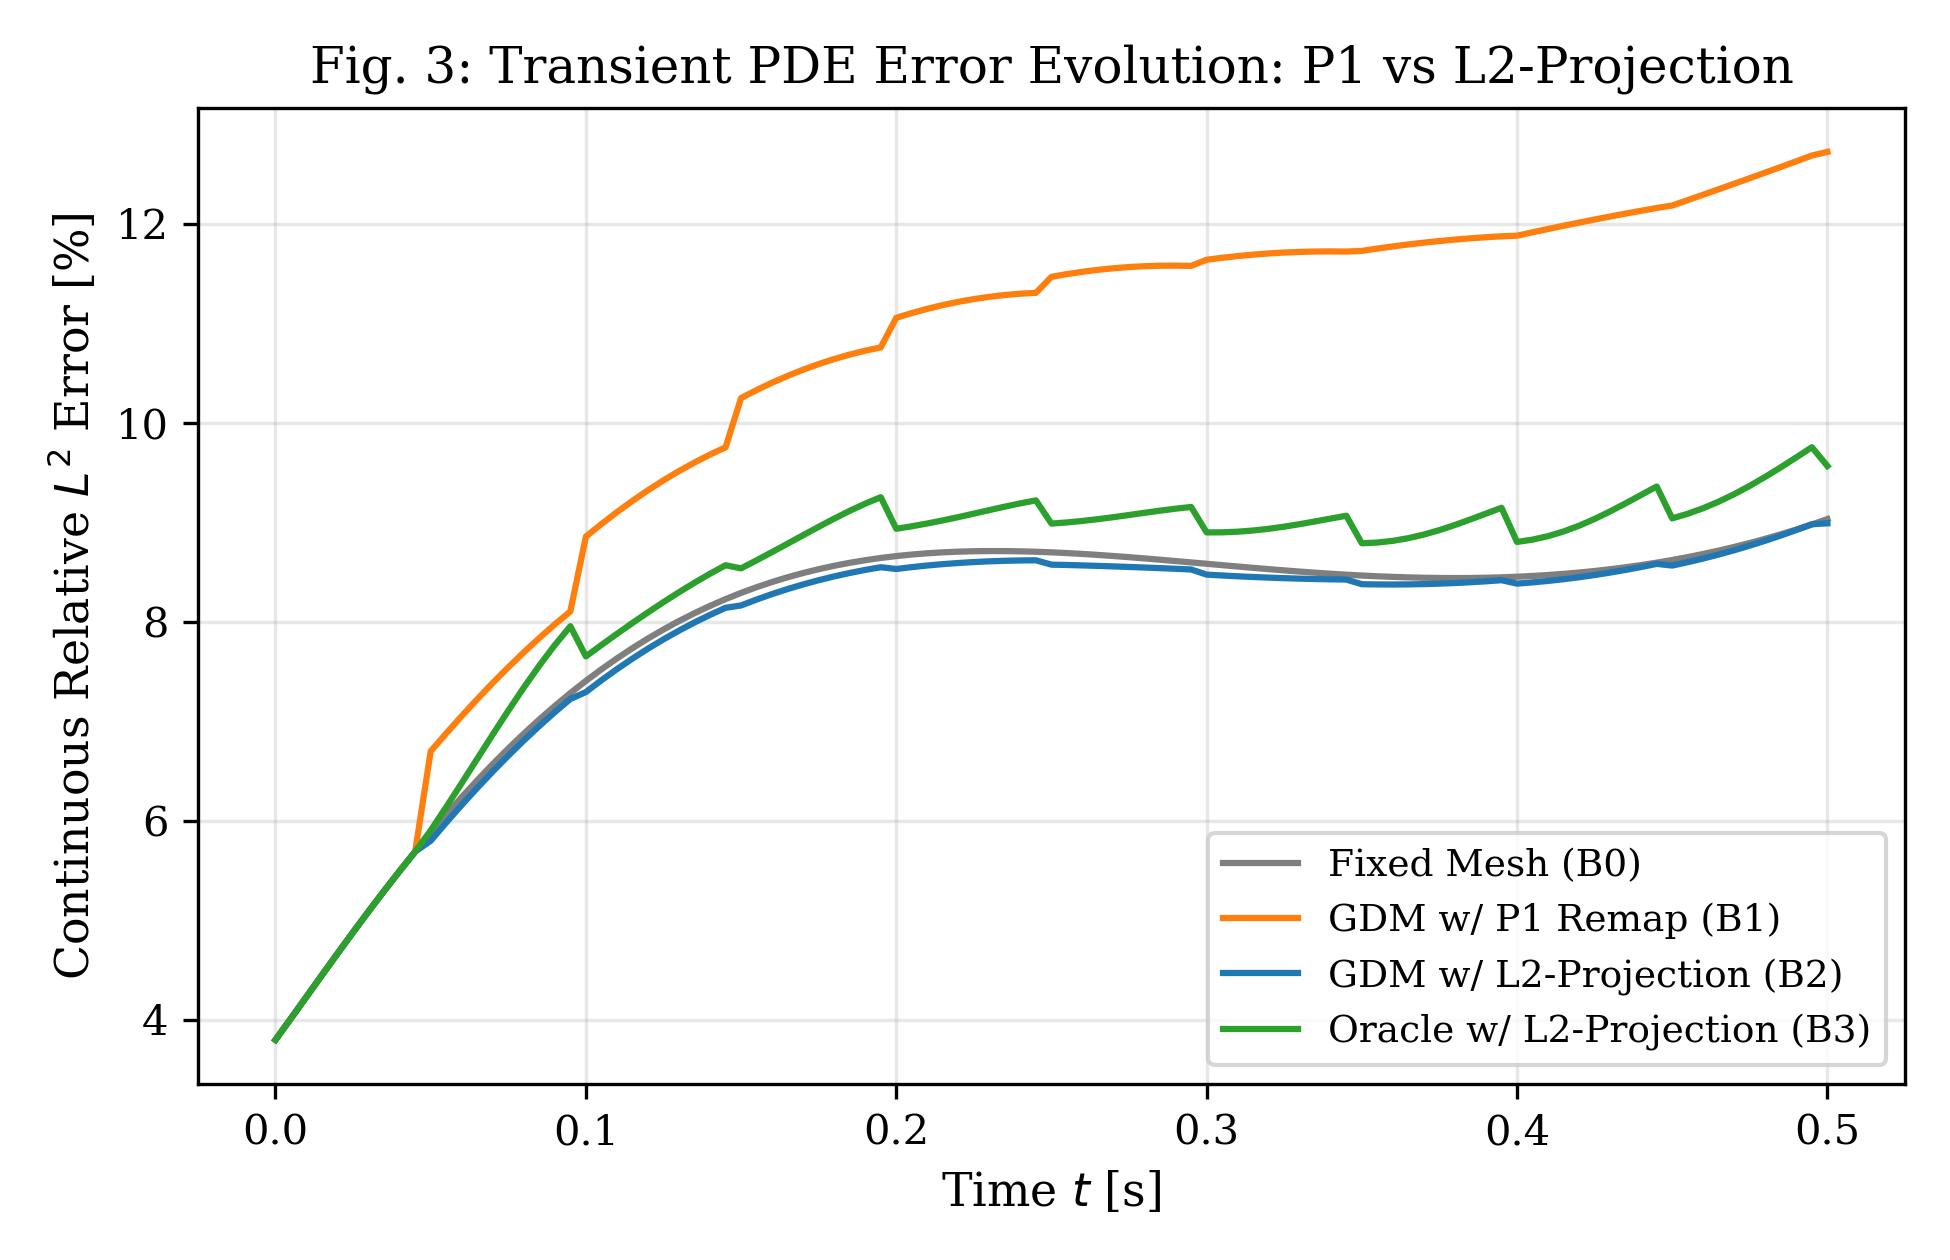
\includegraphics[width=0.92\linewidth]{images/stage_b/fig3_dynamic_pde_error.png}
\caption{Evoluzione temporale dell'errore relativo $L^2$ nelle configurazioni dinamiche considerate.}
\label{fig:final_error_dynamics}
\end{figure}

La curva associata al remapping $P_1$ evidenzia una crescita dell'errore compatibile con l'accumulo del contributo introdotto dai trasferimenti successivi. Nel caso della proiezione $L^2$, l'errore rimane invece più vicino a quello della mesh fissa, sebbene siano osservabili variazioni localizzate in corrispondenza degli eventi di trasferimento.

La formulazione ALE presenta un'evoluzione temporale più regolare, poiché il cambiamento geometrico viene distribuito nel tempo e non richiede una fase separata di riproiezione dello stato. Il prezzo di tale continuità è, nel benchmark considerato, un errore leggermente superiore alla configurazione con proiezione $L^2$.

Nel complesso, il confronto conferma che la scelta del meccanismo di accoppiamento tra mesh mobile e stato fisico costituisce una componente determinante del comportamento end-to-end. La qualità della geometria prodotta dalla GNN non è quindi sufficiente, da sola, a caratterizzare la precisione della simulazione.

\subsection{Costo computazionale e scomposizione del runtime}

\label{subsec:runtime_analysis}

L'accuratezza viene valutata congiuntamente al costo computazionale introdotto dall'adattamento. Il tempo totale di simulazione può essere scomposto concettualmente come

\begin{equation}
T_{\mathrm{total}}
=
T_{\mathrm{FEM}}
+
T_{\mathrm{GNN}}
+
T_{\mathrm{Safety}}
+
T_{\mathrm{Remap}}
+
T_{\mathrm{other}},
\label{eq:runtime_decomposition}
\end{equation}

dove $T_{\mathrm{FEM}}$ rappresenta il costo associato all'assemblaggio e alla soluzione del sistema FEM, $T_{\mathrm{GNN}}$ il costo di inferenza del mesh mover, $T_{\mathrm{Safety}}$ il costo del filtro geometrico e $T_{\mathrm{Remap}}$ il costo dell'eventuale trasferimento esplicito dello stato.

Per la formulazione ALE, il termine $T_{\mathrm{Remap}}$ è assente dalla pipeline, poiché lo stato non viene proiettato esplicitamente tra due configurazioni successive. Restano naturalmente i costi associati all'aggiornamento della geometria, al calcolo della velocità di mesh e alla costruzione degli operatori FEM sulla configurazione corrente.

Nel benchmark transiente unificato a $100$ passi temporali, la configurazione GDM + $L^2$ registra un tempo di esecuzione totale pari a

\begin{equation}
\begin{aligned}
T_{\mathrm{total}}^{L^2}
&=
4.18\ \mathrm{s},
\\
T_{\mathrm{Remap}}^{L^2}
&=
3.35\ \mathrm{s},
\end{aligned}
\label{eq:runtime_l2}
\end{equation}

con il trasferimento dello stato che rappresenta circa l'$80.1\%$ del tempo totale della pipeline in questo benchmark.

La formulazione GDM + ALE completa invece la simulazione in

\begin{equation}
T_{\mathrm{total}}^{\mathrm{ALE}}
=
1.76\ \mathrm{s},
\qquad
T_{\mathrm{Remap}}^{\mathrm{ALE}}
\equiv 0.
\label{eq:runtime_ale}
\end{equation}

Il rapporto tra i tempi complessivi definisce lo speedup operativo della formulazione ALE rispetto alla configurazione con proiezione $L^2$:

\begin{equation}
S_{\mathrm{ALE}}
=
\frac{
T_{\mathrm{total}}^{L^2}
}{
T_{\mathrm{total}}^{\mathrm{ALE}}
}
=
\frac{4.18\ \mathrm{s}}{1.76\ \mathrm{s}}
\approx
2.37\times.
\label{eq:ale_speedup}
\end{equation}

\begin{figure}[htbp]
\centering
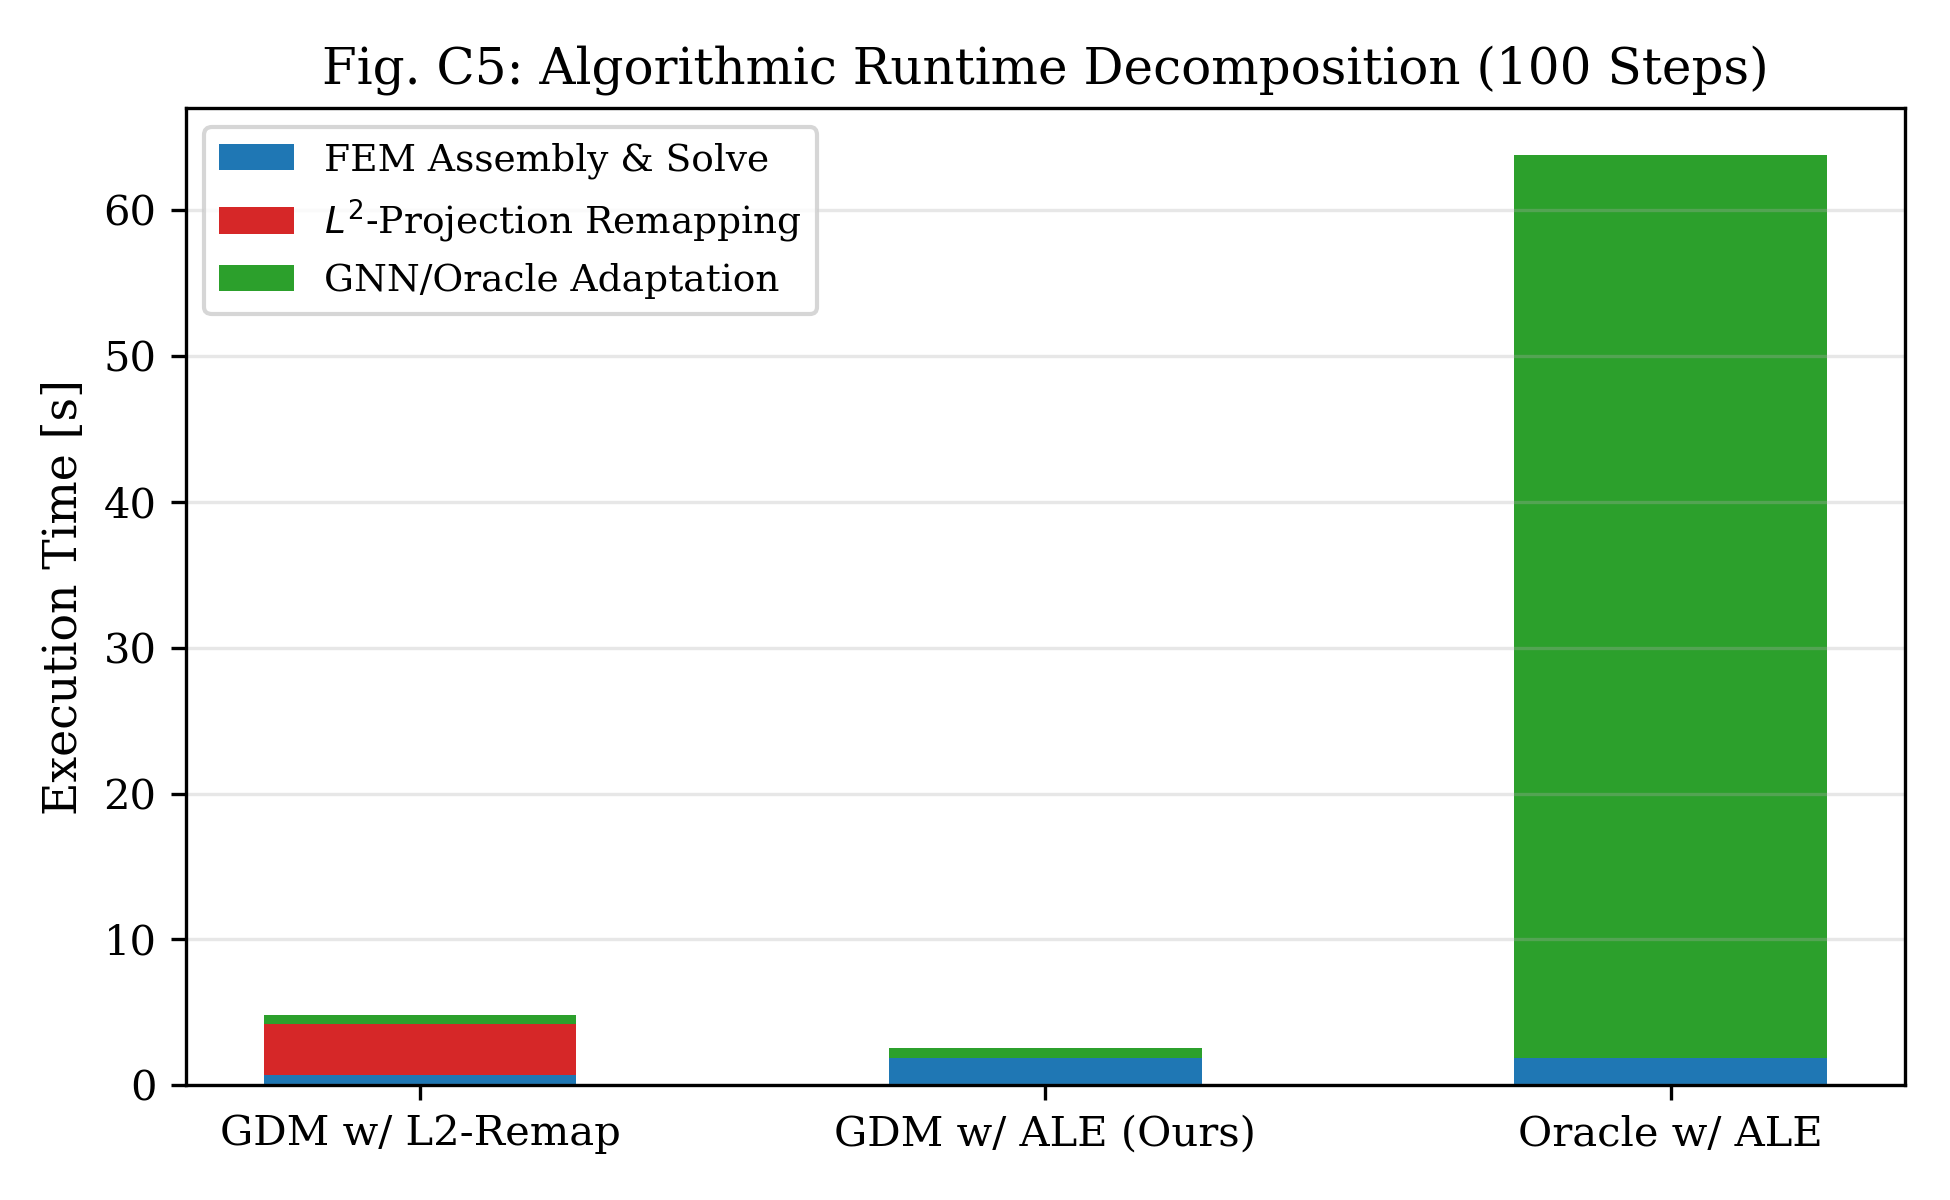
\includegraphics[width=0.90\linewidth]{images/stage_c/fig_c5_runtime_decomposition.png}
\caption{Confronto del costo computazionale tra la strategia con proiezione $L^2$ e la formulazione ALE. Il benchmark mostra uno speedup complessivo di $2.37\times$ per la configurazione ALE.}
\label{fig:final_runtime}
\end{figure}

Il risultato evidenzia che, nel caso considerato, il costo della proiezione dello stato costituisce la componente dominante della pipeline con remapping $L^2$. La formulazione ALE elimina tale operazione separata e riduce il tempo complessivo di simulazione da $4.18$ s a $1.76$ s.

Lo speedup osservato deve tuttavia essere interpretato come un risultato sperimentale specifico del benchmark e non come una stima asintotica generale della convenienza dell'ALE. Esso dipende infatti dalla frequenza di adattamento, dal costo della proiezione, dalla dimensione della discretizzazione e dall'implementazione del solutore.

\subsection{Robustezza geometrica e tracking dinamico della mesh}

\label{subsec:geometric_robustness}

La validazione conclusiva riguarda la qualità geometrica della triangolazione lungo l'intera sequenza temporale. A differenza dello stress test isolato condotto nello Stage A, nel quale la rete veniva volutamente sottoposta a spostamenti amplificati, in questa sezione viene considerato il regime nominale della simulazione dinamica.

Durante l'intera simulazione di $100$ passi temporali, utilizzando il gradiente FEM ricostruito a runtime, il minimo determinante Jacobiano orientato osservato su tutti gli elementi è

\begin{equation}
\min_{t\in(0,T]}
\min_{e=1,\ldots,M}
J_e(t)
\approx
6.59\times10^{-4}
>
\epsilon,
\label{eq:final_min_j}
\end{equation}

con $\epsilon=10^{-4}$. Il valore iniziale della mesh indeformata è

\[
J_0=9.77\times10^{-4}.
\]

Nel benchmark nominale il fattore globale del Safety Filter rimane

\[
\alpha_{\mathrm{global}}(t)=1
\]

per tutte le finestre di adattamento. Ciò significa che le configurazioni previste dalla GNN risultano già ammissibili rispetto alla soglia geometrica e che il filtro non deve ridurre gli spostamenti.

Questo risultato deve essere distinto dalla funzione di protezione verificata nello stress test dello Stage A: in quel caso il filtro veniva attivato intenzionalmente mediante amplificazione dello spostamento, mentre nel benchmark nominale non è stato necessario alcun intervento correttivo.

\begin{figure}[htbp]
\centering
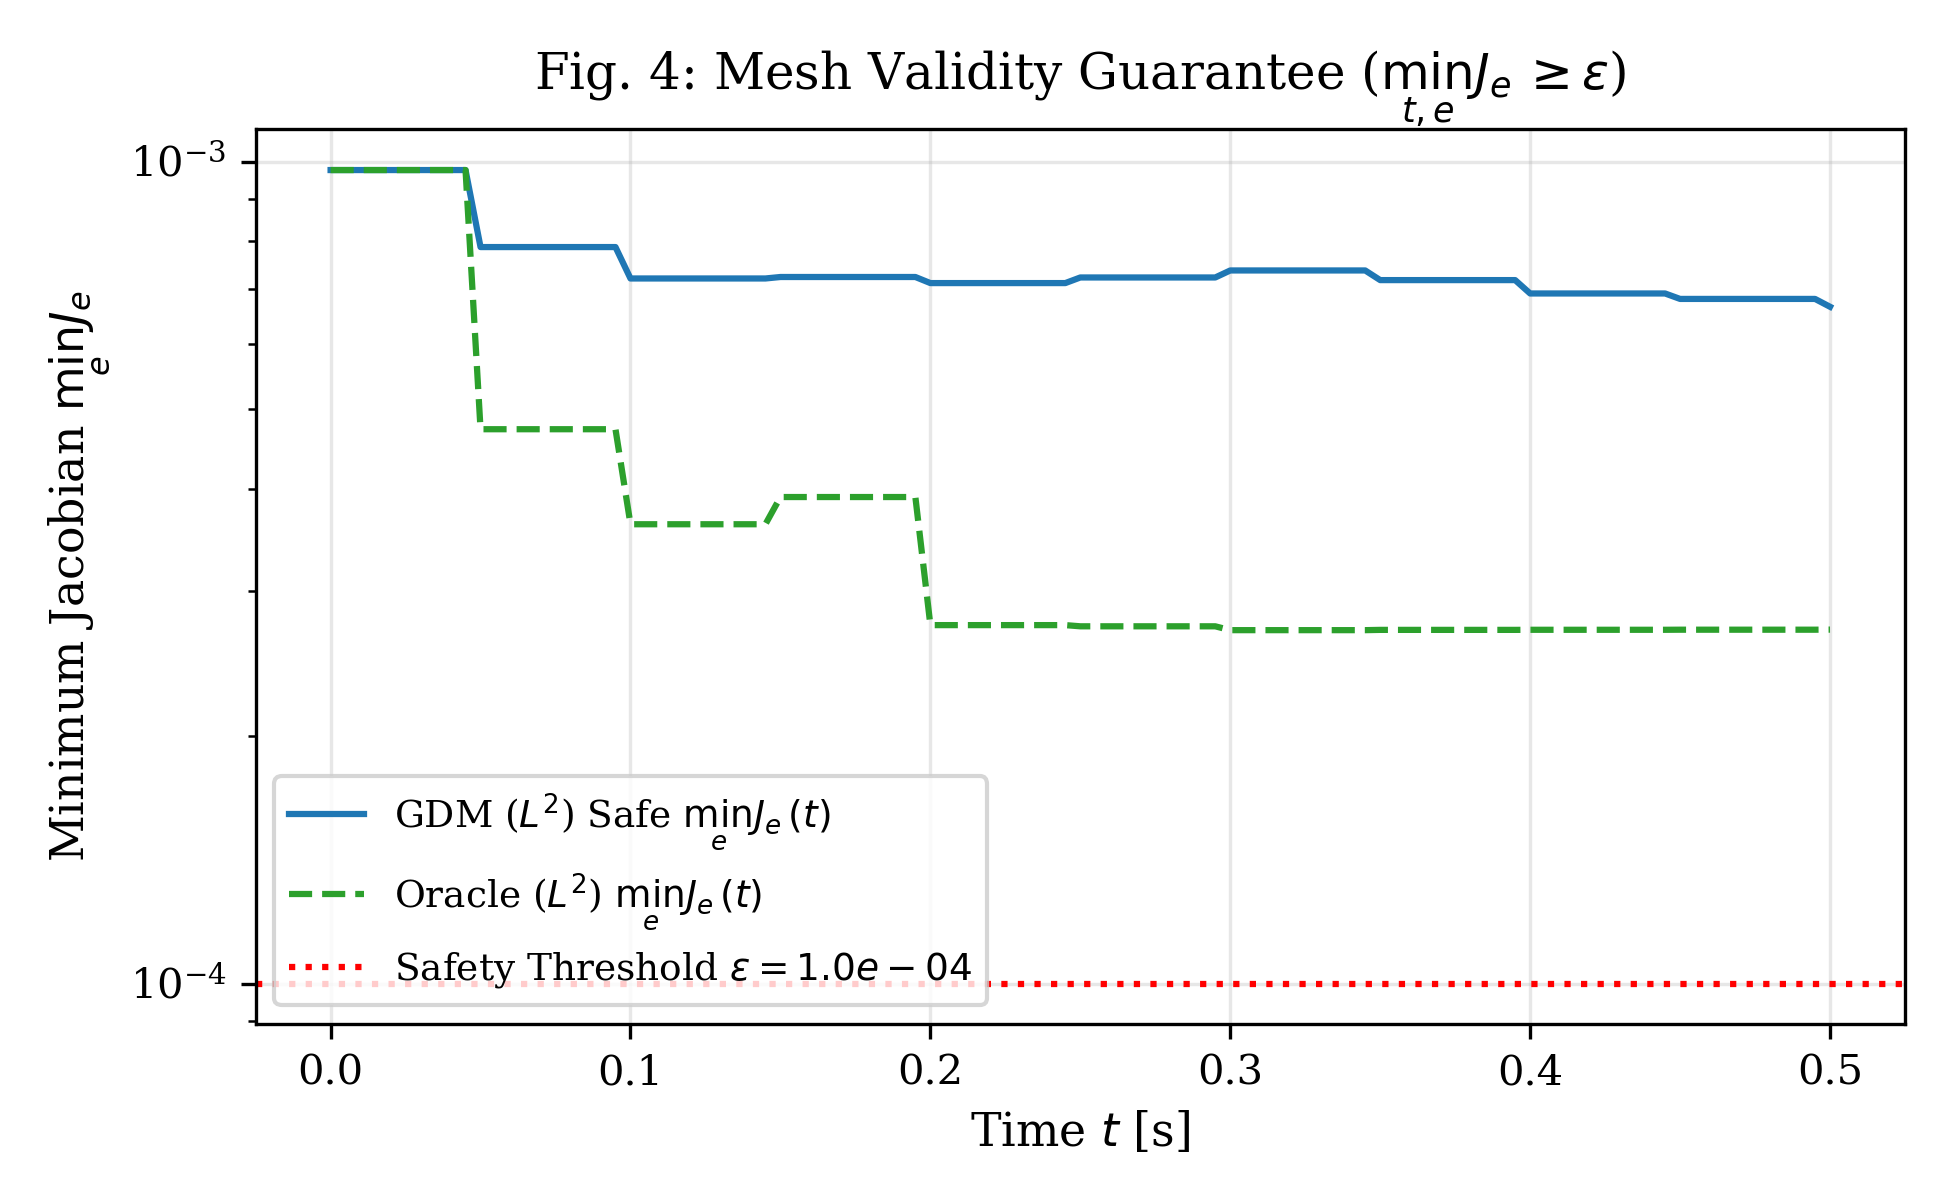
\includegraphics[width=0.92\linewidth]{images/stage_b/fig4_mesh_safety_over_time.png}
\caption{Evoluzione temporale del minimo determinante orientato $J_{\min}(t)$ durante la simulazione dinamica. La linea orizzontale rappresenta la soglia geometrica $\epsilon$.}
\label{fig:final_mesh_safety}
\end{figure}

L'analisi di $J_{\min}(t)$ deve essere interpretata insieme all'evoluzione di $\alpha_{\mathrm{global}}(t)$ e agli istanti di adattamento. Un valore $\alpha_{\mathrm{global}}=1$ indica che la configurazione proposta è direttamente ammissibile; un valore inferiore a uno segnalerebbe invece l'attivazione del filtro e la conseguente contrazione dello spostamento.

La proprietà osservata riguarda esclusivamente la validità geometrica della discretizzazione e non costituisce, di per sé, una proprietà di conservazione della soluzione PDE. La consistenza geometrica e il comportamento del trasferimento dello stato sono stati verificati separatamente nel Capitolo~\ref{sec:diagnostics} mediante i test di Stage B e Stage C.

\begin{figure}[htbp]
\centering
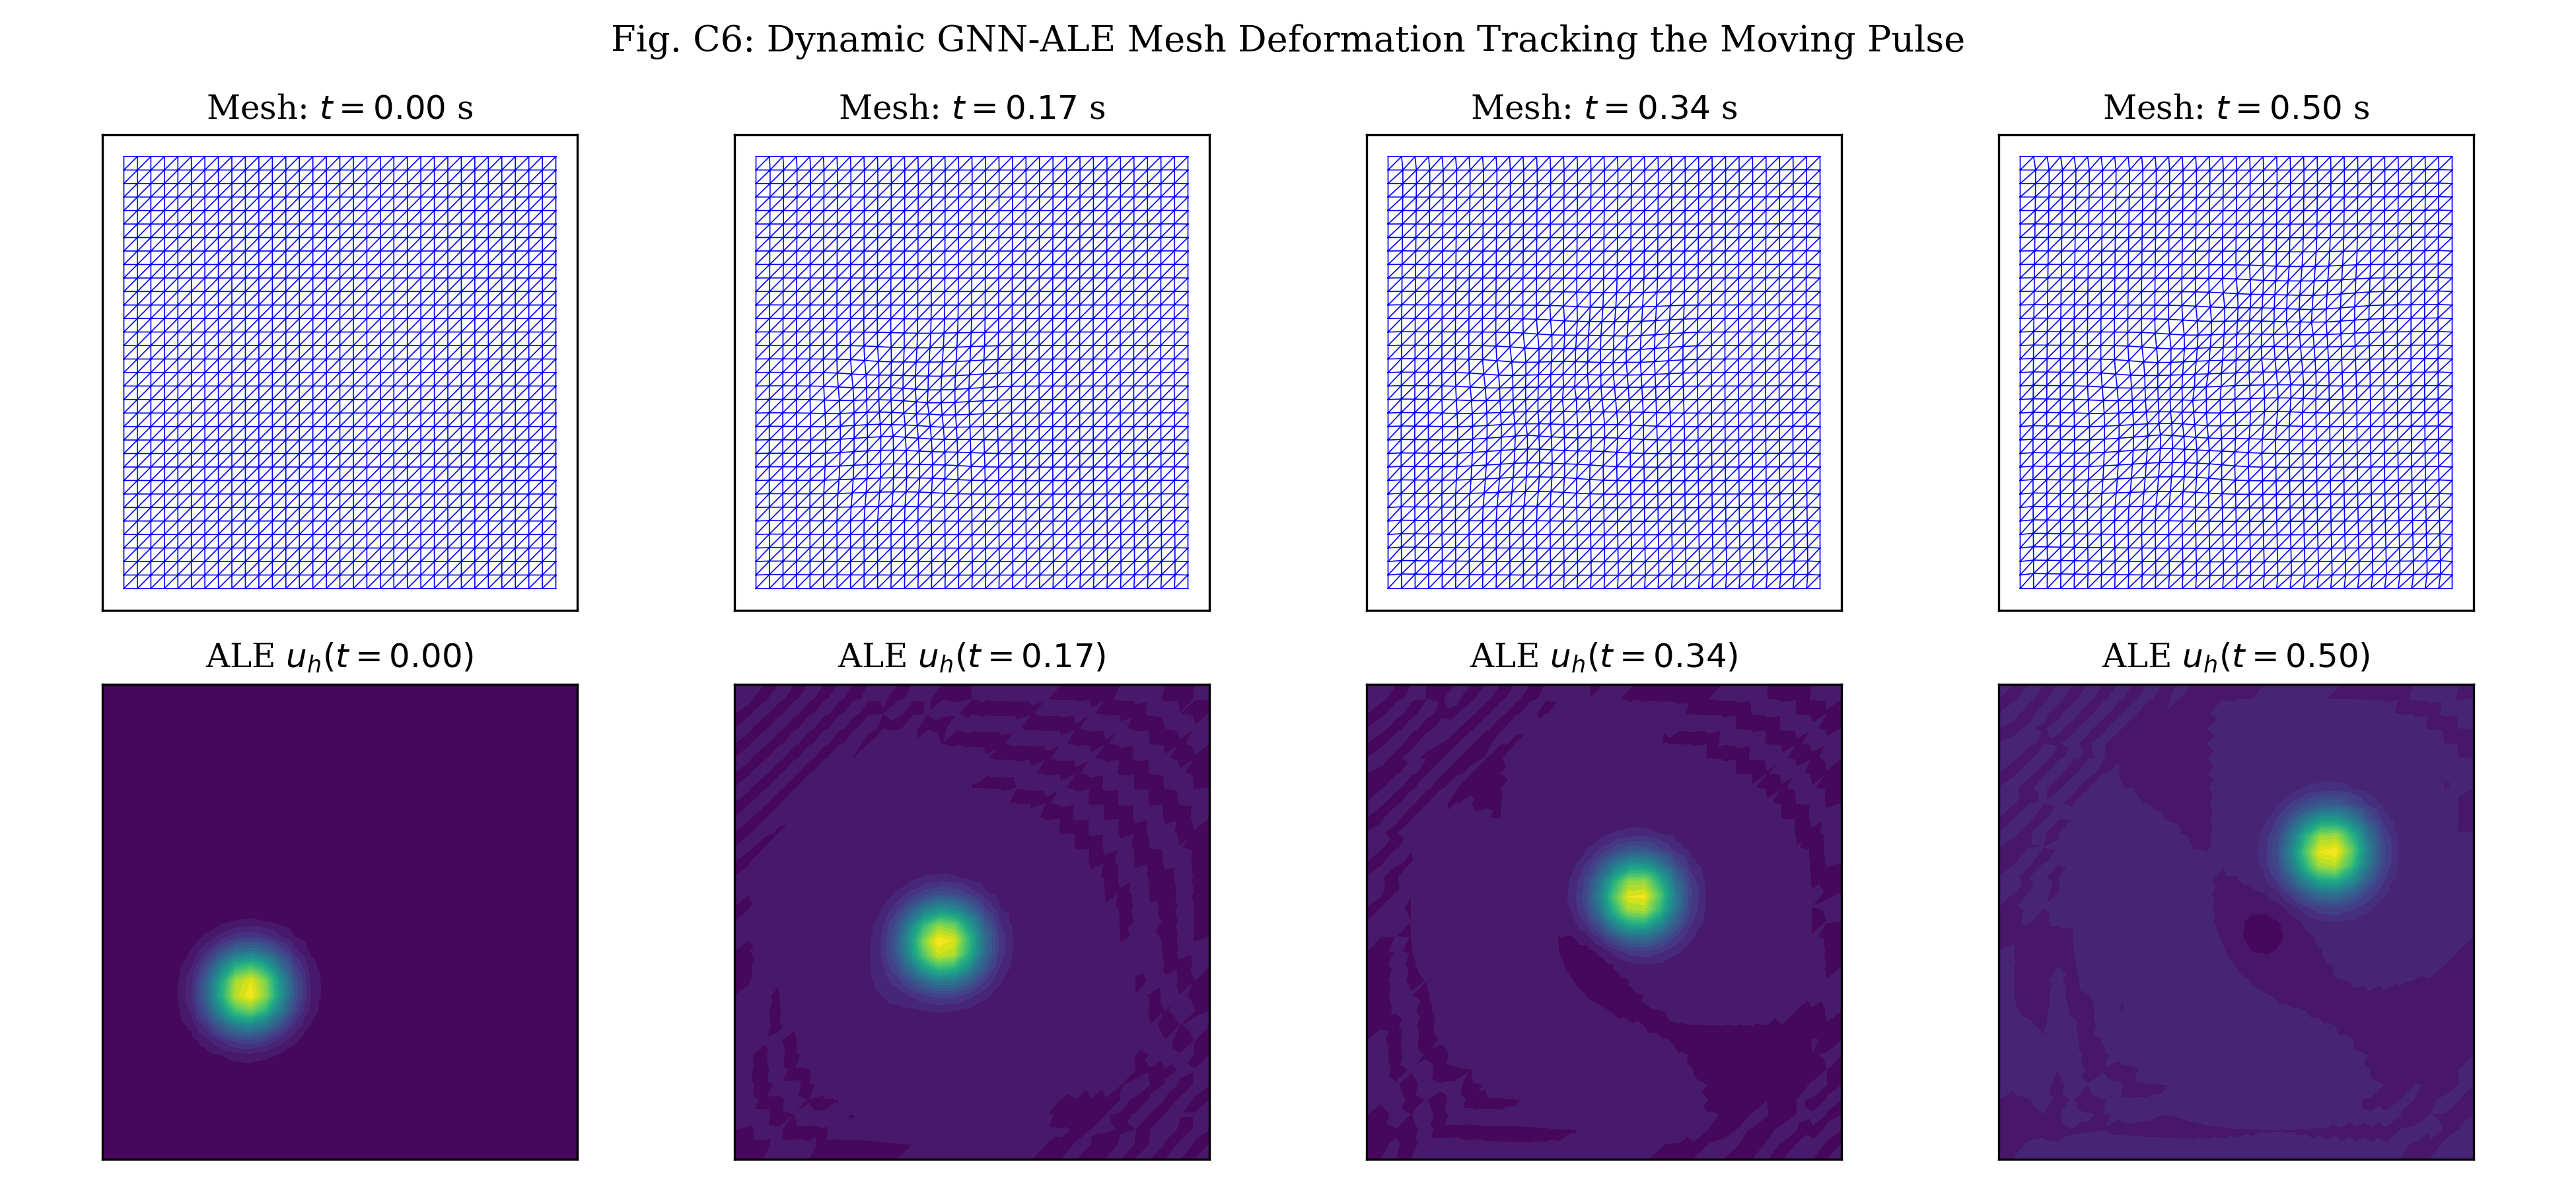
\includegraphics[width=0.90\linewidth]{images/stage_c/fig_c6_qualitative_tracking.png}
\caption{Esempio qualitativo del tracking della struttura della soluzione durante l'evoluzione dinamica con mesh adattata.}
\label{fig:final_tracking}
\end{figure}

Nel complesso, il benchmark dinamico mostra che l'integrazione della GNN con il controllo geometrico deterministico mantiene una triangolazione ammissibile durante l'intera simulazione considerata. Nel regime nominale analizzato, il Safety Filter non altera la traiettoria predetta dalla GNN; il principale effetto della scelta tra remapping $L^2$ e formulazione ALE riguarda quindi il trattamento dello stato fisico e il conseguente compromesso tra accuratezza e costo computazionale.

\newpage

% =============================================================
% 7. DISCUSSIONE E LIMITAZIONI
% =============================================================
\section{Discussion}
\label{sec:discussion}
% 7.1 Compromesso tra remapping L2 continuo e formulazione ALE.
% 7.2 Perché l'ottimizzazione geometrica istantanea non equivale all'ottimo per l'errore PDE temporale.
% 7.3 Generalizzabilità della GNN a diverse condizioni fluidodinamiche senza retraining.
% 7.4 Limitazioni attuali: approccio mono-dominio 2D, connettività costante (r-adaptation pura senza topologia dinamica h/p).

I risultati sperimentali ottenuti attraverso la validazione disaccoppiata (Stage A--C) e il benchmark dinamico end-to-end evidenziano che l'efficacia dell'$r$-adattività neurale in regime transiente dipende strettamente dall'accoppiamento tra generatore geometrico, certificazione di validità elementare e formulazione discreta dell'equazione di evoluzione.

In primo luogo, il confronto tra gli operatori di trasferimento di stato dimostra che il remapping pointwise baricentrico (\textit{GDM + $P_1$}), pur essendo computazionalmente economico ($0.293$ s su $10$ adattamenti), introduce una dissipazione numerica cumulativa che innalza l'errore finale al $12.62\%$ ($12.54\%$ in replay controllato), rendendo l'adattività controproducente rispetto a una griglia fissa ($9.03\%$). L'adozione della proiezione variazionale globale in norma $L^2$ (\textit{GDM + $L^2$}) elimina tale degrado riportando l'errore al $9.11\%$ ($7.97\%$ integrato nel tempo), ma trasferisce l'onere computazionale sulla fase di remapping ($11.153$ s, pari al $90.0\%$ del tempo totale di simulazione).

La formulazione conservativa \textit{GDM + ALE} risolve strutturalmente questo collo di bottiglia: convertendo lo spostamento nodale filtrato $\Delta\mathbf{X}_{\mathrm{safe}}$ in una velocità di griglia continua a tratti e integrando l'operatore cinematico $C_{\mathrm{mesh}}^{n+\frac12}$ conforme alla D-GCL direttamente nel passo temporale, essa preserva esattamente sia il campo costante sia la massa discreta globale ($\mathbf{1}^T M^n\mathbf{U}^n$), abbattendo il tempo totale di esecuzione da $12.387$ s a $2.226$ s (speedup di $5.56\times$ in ciclo chiuso e $5.60\times$ in replay) a fronte di uno scostamento di errore contenuto in $0.34$ punti percentuali rispetto alla proiezione $L^2$.

È opportuno discutere con trasparenza due limitazioni emerse nella presente formulazione, che delineano direzioni naturali di estensione:
\begin{enumerate}
    \item \textbf{Interazione tra errore di discretizzazione temporale e guadagno spaziale}: mentre nello studio statico (Stage A) la rilocazione nodale riduce nettamente l'errore di interpolazione rispetto alla griglia uniforme, nel benchmark dinamico transiente le configurazioni \textit{GDM + $L^2$} ($7.97\%$) e \textit{GDM + ALE} ($8.26\%$) mostrano un errore globale dello stesso ordine della mesh fissa ($7.96\%$), mentre \textit{Oracle + ALE} scende al $7.74\%$. Ciò è dovuto al fatto che, sulla risoluzione $32\times32$ con schema Backward Euler del primo ordine ($\mathcal{O}(\Delta t)$) e assenza di stabilizzazione upwind (es. SUPG), l'errore di dispersione e dissipazione temporale associato all'avanzamento del fronte domina sul guadagno di interpolazione spaziale $\mathcal{O}(h^2)$. L'adozione di integratori temporali ALE di ordine superiore (quali BDF2 o schemi Crank--Nicolson geometricamente conservativi) e l'applicazione a fronti con scale spaziali ancora più ridotte ($\sigma \ll h$) sono attese amplificare significativamente il vantaggio di accuratezza rispetto alla griglia Euleriana fissa.
    \item \textbf{Natura globale del fattore di contrazione $\alpha_{\mathrm{global}}$}: il \textit{Deterministic Safety Filter} garantisce analiticamente $\min_e J_e(\alpha_{\mathrm{global}}) \geq \epsilon$ in tempo $\mathcal{O}(M)$ mediante un unico coefficiente scalare globale. Sebbene nei regimi nominali analizzati la regolarizzazione di training mantenga $\alpha_{\mathrm{global}}=1$, in presenza di griglie di grandi dimensioni un singolo elemento critico prossimo alla degenerazione ($\alpha_e^\star \ll 1$) limiterebbe uniformemente lo spostamento su tutto il dominio. Lo sviluppo di schemi di filtraggio locale con rilassamento ellittico sui soli anelli di adiacenza dell'elemento critico costituisce pertanto un'importante estensione metodologica.
\end{enumerate}

\newpage

% =============================================================
% 8. CONCLUSIONI E SVILUPPI FUTURI
% =============================================================
\section{Conclusions and Future Work}
\label{sec:conclusions}
% 8.1 Riepilogo dei traguardi metodologici e computazionali conseguiti.
% 8.2 Estensione a sistemi non lineari: Navier-Stokes incomprimibili 2D e scia di von Kármán.
% 8.3 Prospettive per griglie tridimensionali (tetraedriche/poliedriche) e inferenza parallela distribuita.

\newpage

% =============================================================
% RINGRAZIAMENTI
% =============================================================
\section*{Acknowledgments}
% Ringraziamenti istituzionali, progetti di ricerca, supporto finanziario o risorse di calcolo.

% =============================================================
% BIBLIOGRAFIA
% =============================================================
\bibliographystyle{unsrtnat}
% \bibliography{references} % Decommentare quando sarà presente il file references.bib

\end{document}